% Generated fragments require trusted human review before compilation.
% This binder never requests shell escape or runs external tools.
\documentclass[11pt]{article}
% Trusted shared apparatus. Requires LuaLaTeX; never use shell escape.
\usepackage{fontspec}
\defaultfontfeatures{Ligatures=TeX}
\IfFontExistsTF{Noto Serif}{\setmainfont{Noto Serif}}{%
  \IfFontExistsTF{DejaVu Serif}{\setmainfont{DejaVu Serif}}{%
    \IfFontExistsTF{Times New Roman}{\setmainfont{Times New Roman}}{%
      \PackageError{gelfand-binder}{No configured Cyrillic serif font installed}{Install Noto Serif or DejaVu Serif, or select an installed Cyrillic font.}%
    }%
  }%
}
\IfFontExistsTF{Noto Sans}{\setsansfont{Noto Sans}}{%
  \IfFontExistsTF{DejaVu Sans}{\setsansfont{DejaVu Sans}}{\setsansfont{Arial}}%
}
\IfFontExistsTF{Noto Sans Mono}{\setmonofont{Noto Sans Mono}}{%
  \IfFontExistsTF{DejaVu Sans Mono}{\setmonofont{DejaVu Sans Mono}}{\setmonofont{Courier New}}%
}
\usepackage[a4paper,margin=22mm]{geometry}
\usepackage{amsmath,amssymb,amsthm,mathtools}
\usepackage{xcolor}
\usepackage{tikz}
\usepackage{tikz-cd}
\usetikzlibrary{arrows.meta,positioning,calc}
\usepackage{hyperref}
\hypersetup{unicode=true,colorlinks=true,linkcolor=blue,pdftitle={Gelfand transcription binder}}
\newtheorem{theorem}{Theorem}
\newtheorem{lemma}{Lemma}
\newtheorem{proposition}{Proposition}
\newtheorem{corollary}{Corollary}
\theoremstyle{definition}
\newtheorem{definition}{Definition}
\newtheorem{example}{Example}
\theoremstyle{remark}
\newtheorem{remark}{Remark}
\setlength{\parindent}{0pt}
\setlength{\parskip}{0.55em}
\setlength{\emergencystretch}{3em}
\newcommand{\SourcePage}[2]{%
  \clearpage\phantomsection\label{#1:source-page}%
  \addcontentsline{toc}{subsection}{#1}%
  {\small\sffamily\color{blue!60!black}Source scan frame: #1; visible page/leaf label: #2}\par\medskip%
}
\newcommand{\Unclear}[3]{%
  \begingroup\color{orange!70!black}%
  [Unresolved reading #1/#2: #3]\endgroup%
}
\newcommand{\Incomplete}[3]{%
  \par\begingroup\color{red!65!black}\textbf{Incomplete #1/#2:} #3\endgroup\par%
}
\newcommand{\SourceFigure}[3]{%
  \par\begingroup\color{blue!60!black}\textbf{\hyperref[#1:source-page]{Source figure #1/#2}:} #3%
  \par\textit{Consult the authoritative scan at this locator.}\endgroup\par%
}



% Reader layout only. Original diplomatic text is retained verbatim.
\setlength{\parskip}{0.35em}
\setlength{\emergencystretch}{4em}
\renewcommand{\SourcePage}[2]{%
  \par\addvspace{1em}\phantomsection\label{#1:source-page}%
  \addcontentsline{toc}{subsection}{#1}%
  {\footnotesize\sffamily\color{blue!55!black}#1%
    \def\givenlabel{#2}\def\nolabel{unlabelled}%
    \ifx\givenlabel\nolabel\else\quad[номер в источнике: #2]\fi
  }\par\nobreak\smallskip%
}
\renewcommand{\Unclear}[3]{%
  \begingroup\color{orange!65!black}%
  \ifmmode\text{[неясно: #3]}\else[неясно: #3]\fi\endgroup%
}
\renewcommand{\Incomplete}[3]{%
  \par\begingroup\color{red!60!black}\textbf{Неразобранный фрагмент:} #3%
  \endgroup\par%
}
\renewcommand{\SourceFigure}[3]{%
  \par\begingroup\color{blue!55!black}\textbf{Рисунок:} #3%
  \par{\small\textit{Исходный рисунок: \hyperref[#1:source-page]{#1}, #2.}}%
  \endgroup\par%
}
\hypersetup{pdftitle={Семинар И. М. Гельфанда. Дипломатическая транскрипция},pdfauthor={},pdfsubject={Русское рабочее издание с отмеченными сомнительными чтениями}}

\usepackage[normalem]{ulem}
\usepackage{newunicodechar}
\usepackage{adjustbox}
\newfontfamily\SourceSymbolFont{Segoe UI Symbol}
\newfontfamily\SourceCJKFont{MS Gothic}
\let\DiplomaticMathUnderline\underline
\renewcommand{\underline}[1]{\ifmmode\DiplomaticMathUnderline{#1}\else\uline{#1}\fi}
\newunicodechar{→}{\ifmmode\text{{\SourceSymbolFont\char"2192}}\else{\SourceSymbolFont\char"2192}\fi}
\newunicodechar{⇒}{\ifmmode\text{{\SourceSymbolFont\char"21D2}}\else{\SourceSymbolFont\char"21D2}\fi}
\newunicodechar{∀}{\ifmmode\text{{\SourceSymbolFont\char"2200}}\else{\SourceSymbolFont\char"2200}\fi}
\newunicodechar{∂}{\ifmmode\text{{\SourceSymbolFont\char"2202}}\else{\SourceSymbolFont\char"2202}\fi}
\newunicodechar{∈}{\ifmmode\text{{\SourceSymbolFont\char"2208}}\else{\SourceSymbolFont\char"2208}\fi}
\newunicodechar{∌}{\ifmmode\text{{\SourceSymbolFont\char"220C}}\else{\SourceSymbolFont\char"220C}\fi}
\newunicodechar{√}{\ifmmode\text{{\SourceSymbolFont\char"221A}}\else{\SourceSymbolFont\char"221A}\fi}
\newunicodechar{∞}{\ifmmode\text{{\SourceSymbolFont\char"221E}}\else{\SourceSymbolFont\char"221E}\fi}
\newunicodechar{∧}{\ifmmode\text{{\SourceSymbolFont\char"2227}}\else{\SourceSymbolFont\char"2227}\fi}
\newunicodechar{∩}{\ifmmode\text{{\SourceSymbolFont\char"2229}}\else{\SourceSymbolFont\char"2229}\fi}
\newunicodechar{∪}{\ifmmode\text{{\SourceSymbolFont\char"222A}}\else{\SourceSymbolFont\char"222A}\fi}
\newunicodechar{∫}{\ifmmode\text{{\SourceSymbolFont\char"222B}}\else{\SourceSymbolFont\char"222B}\fi}
\newunicodechar{∴}{\ifmmode\text{{\SourceSymbolFont\char"2234}}\else{\SourceSymbolFont\char"2234}\fi}
\newunicodechar{∼}{\ifmmode\text{{\SourceSymbolFont\char"223C}}\else{\SourceSymbolFont\char"223C}\fi}
\newunicodechar{≈}{\ifmmode\text{{\SourceSymbolFont\char"2248}}\else{\SourceSymbolFont\char"2248}\fi}
\newunicodechar{≠}{\ifmmode\text{{\SourceSymbolFont\char"2260}}\else{\SourceSymbolFont\char"2260}\fi}
\newunicodechar{≤}{\ifmmode\text{{\SourceSymbolFont\char"2264}}\else{\SourceSymbolFont\char"2264}\fi}
\newunicodechar{≥}{\ifmmode\text{{\SourceSymbolFont\char"2265}}\else{\SourceSymbolFont\char"2265}\fi}
\newunicodechar{⊕}{\ifmmode\text{{\SourceSymbolFont\char"2295}}\else{\SourceSymbolFont\char"2295}\fi}
\newunicodechar{⊗}{\ifmmode\text{{\SourceSymbolFont\char"2297}}\else{\SourceSymbolFont\char"2297}\fi}
\newunicodechar{①}{\ifmmode\text{{\SourceSymbolFont\char"2460}}\else{\SourceSymbolFont\char"2460}\fi}
\newunicodechar{②}{\ifmmode\text{{\SourceSymbolFont\char"2461}}\else{\SourceSymbolFont\char"2461}\fi}
\newunicodechar{③}{\ifmmode\text{{\SourceSymbolFont\char"2462}}\else{\SourceSymbolFont\char"2462}\fi}
\newunicodechar{④}{\ifmmode\text{{\SourceSymbolFont\char"2463}}\else{\SourceSymbolFont\char"2463}\fi}
\newunicodechar{Ⓗ}{\ifmmode\text{{\SourceSymbolFont\char"24BD}}\else{\SourceSymbolFont\char"24BD}\fi}
\newunicodechar{〃}{\ifmmode\text{{\SourceCJKFont\char"3003}}\else{\SourceCJKFont\char"3003}\fi}


% Reader revision 3. Annotation wording and candidates remain unchanged.
\setmainfont{NotoSerif-Regular.ttf}[Path=C:/Windows/Fonts/,ItalicFont=NotoSerif-Italic.ttf,BoldFont=NotoSerif-Bold.ttf,BoldItalicFont=NotoSerif-BoldItalic.ttf]
\usetikzlibrary{shapes.geometric,decorations.pathreplacing,decorations.markings,patterns,fit}
\newsavebox{\ReaderAnnotationBox}
\newcommand{\ReaderAnnotation}[1]{%
  \sbox{\ReaderAnnotationBox}{[неясно: #1]}%
  \ifdim\wd\ReaderAnnotationBox>.70\linewidth
    \parbox[t]{.70\linewidth}{\raggedright[неясно: #1]}%
  \else\usebox{\ReaderAnnotationBox}\fi%
}
\ExplSyntaxOn
\cs_new_protected:Npn \reader_unclear_candidate:n #1
 {
  \tl_set:Nx \l_tmpa_tl { \tl_to_str:n {#1} }
  % Text explicitly guarded inside a mathematical candidate remains math-safe.
  \regex_replace_all:nnN { \\(?:text|textrm|textnormal|textbf|operatorname)\s*\{[^{}]*\} } { } \l_tmpa_tl
  \regex_match:nVTF { [\x{0400}-\x{052F}] | \$ } \l_tmpa_tl
   { \ifmmode \text{\ReaderAnnotation{#1}} \else \ReaderAnnotation{#1} \fi }
   {
    \ifmmode
      [\text{неясно:~}#1]
    \else
      \regex_match:nVTF { [_^] | \\ } \l_tmpa_tl
       { \ensuremath{[\text{неясно:~}#1]} }
       { \ReaderAnnotation{#1} }
    \fi
   }
 }
\RenewDocumentCommand \Unclear { m m m }
 { \begingroup\color{orange!65!black}\reader_unclear_candidate:n{#3}\endgroup }
\ExplSyntaxOff
\newsavebox{\ReaderIncompleteBox}
\newcommand{\ReaderIncompleteNote}[1]{%
 \sbox{\ReaderIncompleteBox}{\textbf{Неразобранный фрагмент:} #1}%
 \ifdim\wd\ReaderIncompleteBox>.70\linewidth
  \parbox[t]{.70\linewidth}{\raggedright\textbf{Неразобранный фрагмент:} #1}%
 \else\usebox{\ReaderIncompleteBox}\fi%
}
\renewcommand{\Incomplete}[3]{%
 \ifmmode\text{\color{red!60!black}\ReaderIncompleteNote{#3}}%
 \else\leavevmode\begingroup\color{red!60!black}\ReaderIncompleteNote{#3}\endgroup\fi%
}
% Ragged right avoids stretching long untranslated abbreviations into margins.
\AtBeginDocument{\raggedright}
\newunicodechar{А}{\ifmmode\text{\char"410\relax}\else\char"410\relax\fi}
\newunicodechar{Б}{\ifmmode\text{\char"411\relax}\else\char"411\relax\fi}
\newunicodechar{В}{\ifmmode\text{\char"412\relax}\else\char"412\relax\fi}
\newunicodechar{Г}{\ifmmode\text{\char"413\relax}\else\char"413\relax\fi}
\newunicodechar{Д}{\ifmmode\text{\char"414\relax}\else\char"414\relax\fi}
\newunicodechar{Е}{\ifmmode\text{\char"415\relax}\else\char"415\relax\fi}
\newunicodechar{Ж}{\ifmmode\text{\char"416\relax}\else\char"416\relax\fi}
\newunicodechar{З}{\ifmmode\text{\char"417\relax}\else\char"417\relax\fi}
\newunicodechar{И}{\ifmmode\text{\char"418\relax}\else\char"418\relax\fi}
\newunicodechar{Й}{\ifmmode\text{\char"419\relax}\else\char"419\relax\fi}
\newunicodechar{К}{\ifmmode\text{\char"41A\relax}\else\char"41A\relax\fi}
\newunicodechar{Л}{\ifmmode\text{\char"41B\relax}\else\char"41B\relax\fi}
\newunicodechar{М}{\ifmmode\text{\char"41C\relax}\else\char"41C\relax\fi}
\newunicodechar{Н}{\ifmmode\text{\char"41D\relax}\else\char"41D\relax\fi}
\newunicodechar{О}{\ifmmode\text{\char"41E\relax}\else\char"41E\relax\fi}
\newunicodechar{П}{\ifmmode\text{\char"41F\relax}\else\char"41F\relax\fi}
\newunicodechar{Р}{\ifmmode\text{\char"420\relax}\else\char"420\relax\fi}
\newunicodechar{С}{\ifmmode\text{\char"421\relax}\else\char"421\relax\fi}
\newunicodechar{Т}{\ifmmode\text{\char"422\relax}\else\char"422\relax\fi}
\newunicodechar{У}{\ifmmode\text{\char"423\relax}\else\char"423\relax\fi}
\newunicodechar{Ф}{\ifmmode\text{\char"424\relax}\else\char"424\relax\fi}
\newunicodechar{Х}{\ifmmode\text{\char"425\relax}\else\char"425\relax\fi}
\newunicodechar{Ц}{\ifmmode\text{\char"426\relax}\else\char"426\relax\fi}
\newunicodechar{Ч}{\ifmmode\text{\char"427\relax}\else\char"427\relax\fi}
\newunicodechar{Ш}{\ifmmode\text{\char"428\relax}\else\char"428\relax\fi}
\newunicodechar{Щ}{\ifmmode\text{\char"429\relax}\else\char"429\relax\fi}
\newunicodechar{Ъ}{\ifmmode\text{\char"42A\relax}\else\char"42A\relax\fi}
\newunicodechar{Ы}{\ifmmode\text{\char"42B\relax}\else\char"42B\relax\fi}
\newunicodechar{Ь}{\ifmmode\text{\char"42C\relax}\else\char"42C\relax\fi}
\newunicodechar{Э}{\ifmmode\text{\char"42D\relax}\else\char"42D\relax\fi}
\newunicodechar{Ю}{\ifmmode\text{\char"42E\relax}\else\char"42E\relax\fi}
\newunicodechar{Я}{\ifmmode\text{\char"42F\relax}\else\char"42F\relax\fi}
\newunicodechar{а}{\ifmmode\text{\char"430\relax}\else\char"430\relax\fi}
\newunicodechar{б}{\ifmmode\text{\char"431\relax}\else\char"431\relax\fi}
\newunicodechar{в}{\ifmmode\text{\char"432\relax}\else\char"432\relax\fi}
\newunicodechar{г}{\ifmmode\text{\char"433\relax}\else\char"433\relax\fi}
\newunicodechar{д}{\ifmmode\text{\char"434\relax}\else\char"434\relax\fi}
\newunicodechar{е}{\ifmmode\text{\char"435\relax}\else\char"435\relax\fi}
\newunicodechar{ж}{\ifmmode\text{\char"436\relax}\else\char"436\relax\fi}
\newunicodechar{з}{\ifmmode\text{\char"437\relax}\else\char"437\relax\fi}
\newunicodechar{и}{\ifmmode\text{\char"438\relax}\else\char"438\relax\fi}
\newunicodechar{й}{\ifmmode\text{\char"439\relax}\else\char"439\relax\fi}
\newunicodechar{к}{\ifmmode\text{\char"43A\relax}\else\char"43A\relax\fi}
\newunicodechar{л}{\ifmmode\text{\char"43B\relax}\else\char"43B\relax\fi}
\newunicodechar{м}{\ifmmode\text{\char"43C\relax}\else\char"43C\relax\fi}
\newunicodechar{н}{\ifmmode\text{\char"43D\relax}\else\char"43D\relax\fi}
\newunicodechar{о}{\ifmmode\text{\char"43E\relax}\else\char"43E\relax\fi}
\newunicodechar{п}{\ifmmode\text{\char"43F\relax}\else\char"43F\relax\fi}
\newunicodechar{р}{\ifmmode\text{\char"440\relax}\else\char"440\relax\fi}
\newunicodechar{с}{\ifmmode\text{\char"441\relax}\else\char"441\relax\fi}
\newunicodechar{т}{\ifmmode\text{\char"442\relax}\else\char"442\relax\fi}
\newunicodechar{у}{\ifmmode\text{\char"443\relax}\else\char"443\relax\fi}
\newunicodechar{ф}{\ifmmode\text{\char"444\relax}\else\char"444\relax\fi}
\newunicodechar{х}{\ifmmode\text{\char"445\relax}\else\char"445\relax\fi}
\newunicodechar{ц}{\ifmmode\text{\char"446\relax}\else\char"446\relax\fi}
\newunicodechar{ч}{\ifmmode\text{\char"447\relax}\else\char"447\relax\fi}
\newunicodechar{ш}{\ifmmode\text{\char"448\relax}\else\char"448\relax\fi}
\newunicodechar{щ}{\ifmmode\text{\char"449\relax}\else\char"449\relax\fi}
\newunicodechar{ъ}{\ifmmode\text{\char"44A\relax}\else\char"44A\relax\fi}
\newunicodechar{ы}{\ifmmode\text{\char"44B\relax}\else\char"44B\relax\fi}
\newunicodechar{ь}{\ifmmode\text{\char"44C\relax}\else\char"44C\relax\fi}
\newunicodechar{э}{\ifmmode\text{\char"44D\relax}\else\char"44D\relax\fi}
\newunicodechar{ю}{\ifmmode\text{\char"44E\relax}\else\char"44E\relax\fi}
\newunicodechar{я}{\ifmmode\text{\char"44F\relax}\else\char"44F\relax\fi}
\newunicodechar{Ё}{\ifmmode\text{\char"401\relax}\else\char"401\relax\fi}
\newunicodechar{ё}{\ifmmode\text{\char"451\relax}\else\char"451\relax\fi}

\newunicodechar{æ}{\ifmmode\text{\char"E6\relax}\else\char"E6\relax\fi}
\newunicodechar{−}{\ifmmode\mathbin{\text{\SourceSymbolFont\char"2212\relax}}\else{\SourceSymbolFont\char"2212\relax}\fi}


% Reader-only pairing support; accepted raw bodies remain unchanged.
\RequirePackage{graphicx}
\RequirePackage{adjustbox}
\newcommand{\ReaderOriginalPanel}[2]{%
  \begin{minipage}[t]{.48\linewidth}\vspace{0pt}\centering
    \includegraphics[width=\linewidth,keepaspectratio]{#1}\par\smallskip
    {\scriptsize Оригинал рукописного рисунка: #2}\par
  \end{minipage}%
}
\newcommand{\ReaderDiagramPair}[3]{%
  \par\noindent\begingroup
  \ReaderOriginalPanel{#1}{#2}\hfill
  \begin{minipage}[t]{.48\linewidth}\vspace{0pt}\centering
    {\scriptsize Типографское воссоздание}\par\smallskip
    \begin{adjustbox}{max width=\linewidth}#3\end{adjustbox}\par
  \end{minipage}%
  \endgroup\par\smallskip
}
\newcommand{\ReaderDescriptionPair}[3]{%
  \par\noindent\begingroup
  \ReaderOriginalPanel{#1}{#2}\hfill
  \begin{minipage}[t]{.48\linewidth}\vspace{0pt}\raggedright
    {\scriptsize Типографское описание}\par\smallskip
    #3\par
  \end{minipage}%
  \endgroup\par\smallskip
}


\begin{document}
\begin{center}
{\Large Семинар И. М. Гельфанда}\par\medskip
{\LARGE Дипломатическая транскрипция}\par\bigskip
{\large Рабочее русское издание}\par\medskip
{\large Том 10 из 34. Архивная глава 010}\par\bigskip
Кадры GELFAND-P000659 -- GELFAND-P000704\par
\end{center}
\medskip
Сокращения, отменённые записи и сомнительные чтения сохранены.
Неразобранные фрагменты отмечены в тексте. Математические утверждения
источника переданы без молчаливых исправлений.

В текущем комплекте приняты 165 из 165 возвратов; учтены 1527 из 1527 кадров. Кадров без принятого возврата: 0.
Статусы кадров в отчётах о полноте: транскрибированы 1168, неразборчивы 357, частично прочитаны 1, недоступны 1.
Нерешённых записей журнала чтений: 6820.
Статус «неразборчивый» может отмечать локальную утрату зачёркнутой записи;
он не означает отсутствия всего кадра.
Сверка с рукописью продолжается. Рабочие журналы чтений и происхождения
данных сохранены отдельно.

Ограничения исходного комплекта: повреждённый исходный скан GELFAND-P000722; каталожные записи 603, 694 без сканов; в архивной главе 029 не перечислена часть 25.

Границы кадров показаны небольшими синими указателями; печатный текст
продолжается без обязательного разрыва страницы после каждого кадра.
\bigskip\hrule\bigskip
\SourcePage{GELFAND-P000659}{unlabelled}
\underline{6/IX-76 г. Сем. Гельфанда.}

\underline{Что надо знать из физики.} [Справа: (По Синаю?)]

1) Классическая механика и гам. формализм.

Арнольд ($\leq30$ стр.), Ландау и Лифшиц.

2) Квантовая механика и теория рассеяния…

Ландау и Лифшиц, Квантовая механика (минус первые две главы).

Ферми, Квантовая механика.

3) Теория поля и теория относительности.

Ландау и Лифшиц, Вейнберг, Космология и теория гравитации (1–4 главы).

4) Квантовая теория поля.

[Зачёркнута следующая запись.]
\Incomplete{GELFAND-P000659}{cancelled-four}{Густо зачёркнутая написанная строка под пунктом 4 не читается полностью.}

К след. разу проконсульт. с физиками и сделать на машинке.

\underline{Квантовая теория поля}

1) Вторичное квантование (Бозе и Ферми). — Ландау и Лифшиц.

[Под (Бозе и Ферми) вставлено: статистика.]

2) Запись уравнений через континуальный интеграл,

[Под «уравнений» обведённая вставка: норма.]

ряд теории возмущений, диаграммы Фейнмана.

3) Перенормировки. — Хепп.

4) Поля Янга–Миллса — есть обзоры.

\underline{Гиндикин (и Гельфанд)}. \underline{Всё об $SL(2,\mathbb R)$.}
\begin{equation*}
G=SL(2,\mathbb R),\qquad
\begin{pmatrix}\alpha&\beta\\\gamma&\delta\end{pmatrix},\qquad
\det(\,)=1.
\end{equation*}
(гиперболоид в $\mathbb R^4$).
\begin{equation*}
\alpha\delta-\beta\gamma=1.
\end{equation*}
Он отвечает форме с 2-мя плюсами и 2-мя минусами:
\begin{equation*}
x^2+y^2-z^2-t^2=1.
\end{equation*}
На гиперболоиде действует группа $G\times G$ с пом. левых и правых сдвигов
\begin{equation*}
T_{(g_1,g_2)}g=g_1^{-1}gg_2.
\end{equation*}
\Unclear{GELFAND-P000659}{action-overwrite}{Конечное g с индексом 2 густо наведено; прежние штрихи не установлены.}
Любое лин. преобр., сохр. гиперб., можно записать в таком виде.

Стац. подгруппа точки $e=\begin{pmatrix}1&0\\0&1\end{pmatrix}$ состоит из преобр.
[В конце строки зачёркнута запись в скобках.]
\Incomplete{GELFAND-P000659}{cancelled-stabilizer}{Зачёркнутая запись в скобках после «преобр.» не читается полностью.}
вида $(g,g)$.

\SourcePage{GELFAND-P000660}{unlabelled}
[Вверху зачёркнута написанная строка.]
\Incomplete{GELFAND-P000660}{cancelled-top}{Начальная густо зачёркнутая строка не читается полностью.}

\underline{Упражнение:} вычислить стац. подгр. других точек.

Рассм. ф-и на гиперболоиде.

При $\beta\ne0$ удобно координаты [зачёркнуто: $\alpha,\beta,\delta$] $\alpha,\delta,\beta$.
\Unclear{GELFAND-P000660}{coordinates}{Первый знак и индивидуальные прежние штрихи в зачёркнутой тройке координат не вполне установлены.}
Ф-и на гиперболоиде можно рассм. как ф-и $\psi(\alpha,\delta,\beta)$.

Функции нужно интегрировать по инвариантной мере:
\begin{equation*}
dg=\frac{d\alpha\,d\beta\,d\delta}{|\beta|}
\end{equation*}
(инвар. отн. движ. гиперболоида).

Будем рассматривать пр-во $H=L^2(G)$ относительно этой меры.
\begin{equation*}
\|\psi\|^2=\int|\psi(g)|^2\,dg.
\end{equation*}
\underline{Задача:} разложить ф-и на подпр-ва, инвар. относительно
[Над строкой обведено и зачёркнуто: неприводимые.]
\begin{equation*}
T_{(g_1,g_2)}\psi(g)=\psi(g_1^{-1}gg_2).
\end{equation*}
В $\mathbb R^4$ рассматриваем гиперплоскости
\begin{equation*}
\xi\alpha+\eta\delta-p\beta-q\gamma=\zeta.
\end{equation*}
Г. Философия: надо разделить на серии (алгебр. задача)

(Бернштейн, Гельфанд, Гиндикин).

Серии на представления — другая (трансценд.) задача.

Этот известный пример (Востряки, Гельфанд и Граев,
Молчанов, Strichartz, Виленкин и др.) — известно уже всё о гиперболоидах.

На непривод. — \underline{не надо.}

Возьмём след. типы сечений.

I. $\Delta=\begin{vmatrix}\xi&p\\q&\eta\end{vmatrix}<0$ — однополостный гиперболоид, 4 параметр.

II. $\Delta=\begin{vmatrix}\xi&p\\q&\eta\end{vmatrix}>0$.

а) $|\zeta|>2\sqrt\Delta$ — однопол. гиперболоид.

б) $|\zeta|<2\sqrt\Delta$ — двупол. гиперб.

в) $|\zeta|=2\sqrt\Delta$ — конус.

[Справа объединены скобкой: а) 4, б) 4, в) 3 параметра.]

III. $\Delta=0$ — «плоская вещь», 2 параметр.
[Обведённая вставка: гиперб. параболоид.]

\SourcePage{GELFAND-P000661}{unlabelled}
$A$ — однопол. гиперболоид (случаи I, IIа), 4-пар.

$B$ — двупол. гиперболоид (—»— IIб), 4-пар.

[Ниже зачёркнута отдельная буква: $A$?]
\Unclear{GELFAND-P000661}{cancel-letter}{Зачёркнутая отдельная буква между B и D: A?}

$D$ — конусы, 3-пар.

$E$ — гиперболич. параболоид (случай III), 3-пар.
\begin{equation*}
\psi\in H.
\end{equation*}
\begin{equation*}
\widehat\psi(\xi,\eta,p,q,\zeta)=
\int\psi(g)\delta(\xi\alpha+\eta\delta-p\beta-q\gamma-\zeta)\,dg.
\end{equation*}
(преобр. Радона ф-и во всём пр-ве).

(Г. По технике восх. к технике раб. Г. и Наймарка 1947 г.)

$H_A,H_B,H_D,H_E$ — ф-и, у к-рых равны 0 интегралы
[зачёркнут отдельный знак: $\varphi$?]
\Unclear{GELFAND-P000661}{cancel-integrals}{Зачёркнутый отдельный знак после «интегралы»: φ?}
по гиперпл. данного сем-ва.

[Зачёркнуто: Зад.?]
\Unclear{GELFAND-P000661}{cancel-question}{Зачёркнутое короткое начало вопроса: Зад.?}
Как описать, какие ф-и 4-х и 3-х перем. появляются?

\underline{Основная теорема 1.}

[Зачёркнута формула: $H=H_A$?]
\Unclear{GELFAND-P000661}{cancel-decomp}{В зачёркнутой формуле читаются H, знак равенства и H с индексом A; состав остальных штрихов не установлен.}
\begin{equation*}
1.\quad H=H_A\overset{\cdot}{+}H_B.
\end{equation*}
\begin{equation*}
2.\quad H_A=H_D=H_E.
\end{equation*}
Ф-я $\widehat\psi$ удовл. ультрагиперб. ур-ю 2-го порядка, к-рое можно выписать.

Сем-ва $A,D,E$ явл. минимальными.

Предельные образующие — 3-пар. сем-во $C$.
\begin{equation*}
\begin{pmatrix}1&z\\0&1\end{pmatrix}
\quad\text{— пример прямой},\qquad
\begin{pmatrix}h&z\\0&h^{-1}\end{pmatrix}
\quad(h\text{ — фиксир.})
\end{equation*}
или
\begin{equation*}
g_1^{-1}\begin{pmatrix}1&z\\0&1\end{pmatrix}g_2
\quad\text{(общ. вид предельн. образующей).}
\end{equation*}
$C$ — прямолин. образующие.
\begin{equation*}
2'.\quad H_A=H_D=H_E=H_C.\qquad\text{(дискретные серии)}
\end{equation*}
\underline{Явное указ. проекторов и описание этих пр-в.}
\begin{equation*}
\alpha\delta-\beta\gamma=1.
\end{equation*}
Рассм. соотв. м-во в $\mathbb C^4$ с тем же ур-ем.

и на нём области:

\SourcePage{GELFAND-P000662}{unlabelled}
\begin{equation*}
(\Im\alpha\bar\beta)(\Im\delta\bar\beta)>(\Im\beta)^2.\qquad(1)
\end{equation*}
[Неравенство охвачено скобкой снизу.]

Рассм. их в $\mathbb C^3$.

Она распад. на 2 обл., остовами к-рых являются вещ. пр-ва $\mathbb R^3$.

Нер-во инвар. отн. дробно-лин. преобр. (одна из обл. Зигеля).

Остов $G=SL(2,\mathbb R)$.

Области разделяются знаками скобок.

(Остов области $D$ — наименьшее м-во в $\partial D$, по ограничениям
на к-рое однозн. восст. ф-я, голом. в $D$ и непр. в $\bar D$.)

\underline{Лемма.} В $\mathbb C^3$ с коорд. $(\alpha,\beta,\delta)$
[зачёркнута запись]
\Incomplete{GELFAND-P000662}{cancel-lemma}{Короткая густо зачёркнутая запись перед «нер-во (1)» не читается полностью.}
нер-во (1) есть 2 обл. с остовами $\mathbb R^3$ у каждой.

\underline{Теорема.} На м-ве $\alpha\delta-\beta\gamma=1$ в $\mathbb C^4$ сущ. 2 инвар.
отн. вещ. движ. области, имеющие остовами гиперболоид
[перед уравнением зачёркнут отдельный знак]
\Unclear{GELFAND-P000662}{cancel-theorem}{Зачёркнутый отдельный знак слева от уравнения гиперболоида не установлен.}
$\alpha\delta-\beta\gamma=1$ в $\mathbb R^4$. Обозначим эти области $D_+$ и $D_-$.

\underline{Основная теор. 2.}
\begin{equation*}
\psi\in H_A\ \Longleftrightarrow\ \psi=\psi_++\psi_-,\quad\text{где}
\end{equation*}
$\psi_+$ аналит. прод. в $D_+$, $\psi_-$ аналит. прод. в $D_-$.

[Над следующей строкой: Обозн. [зачёркнута звёздочка] подпр-ва через $H_{A,+}$ и $H_{A,-}$.]

Проектор на $H_{A,+}$ задаётся ф-ей
\begin{equation*}
\int_G K(g_1,g_2)\psi(g_2)\,dg_2,
\end{equation*}
где
\begin{equation*}
K(g_1,g_2)=c\frac{1}{[-\alpha_1\delta_2-\delta_1\alpha_2+\gamma_1\beta_2+\beta_1\gamma_2+2]^{3/2}}.
\end{equation*}
\begin{equation*}
g_1=\begin{pmatrix}\alpha_1&\beta_1\\\gamma_1&\delta_1\end{pmatrix},\qquad g_1\in D_+.
\end{equation*}
Аналогично 2-й проектор.
\begin{equation*}
H_{A,+}\cap H_{A,-}=\{0\},
\end{equation*}
т.к. [зачёркнута запись]
\Incomplete{GELFAND-P000662}{cancel-intersection}{Зачёркнутое слово после «т.к.» не читается полностью.}
всё в $L^2$.

\underline{Подводная часть:} техника интеграла Фурье.

$K(g_1,g_2)$ — аналог ядра Коши.

\underline{Гипотеза Арнольда:} $D_+$ — те, к-рые круг перев. в себя,

$D_-$ — те, к-рые внешн. круга [зачёркнута запись]
\Incomplete{GELFAND-P000662}{cancel-circle}{Короткая зачёркнутая запись перед «перев. в себя» не читается.}
перев. в себя,

$SL(2,\mathbb R)$ — сохр. окружность.

\SourcePage{GELFAND-P000663}{unlabelled}
\underline{13/IX-76 г. Сем. Гельфанда.}

\underline{А.А. Кириллов. Супералгебры, супергруппы и суперпространства.}

\underline{Д.Б. Фукс. Всё об алгебре Вейля.}

$\mathfrak g$ — алгебра Ли. Построим по ней ассоц. алгебру Вейля:
\begin{equation*}
W(\mathfrak g)=\Lambda^*(\mathfrak g')\otimes S^*(\mathfrak g').
\end{equation*}
[Под $\Lambda^*$: внешняя алгебра; под $S^*$: симметрическая алгебра.]

[Следующие две строки заключены в заштрихованную рамку:]

Если в $\mathfrak g$ есть базис $e_1,\ldots,e_n$, то элементы $W(\mathfrak g)$
— функции от $2n$ переменных, супер $\mathfrak g$.

Градуировка: $\Lambda^p(\mathfrak g')\otimes S^q(\mathfrak g')$ имеет степень $p+2q$.

Дифференциал: $d:W(\mathfrak g)\to W(\mathfrak g)$ со свойствами

1) $d^2=0$, 2) обычным образом действует на [зачёркнута запись]
\Incomplete{GELFAND-P000663}{cancel-product}{Зачёркнутая запись перед «произведение» не читается полностью.}
произведение.

Пусть $h\in\mathfrak g'$. Рассмотрим $h\otimes1\in W(\mathfrak g)$.
[Под $\mathfrak g'$ написано: $\Lambda^1(\mathfrak g')$, соединено знаком повторения.]
\begin{equation*}
d:\Lambda^1(\mathfrak g')\otimes S^0(\mathfrak g')\to
\Lambda^2(\mathfrak g')\otimes S^0(\mathfrak g')\oplus
\Lambda^0(\mathfrak g')\otimes S^1(\mathfrak g').
\end{equation*}
\begin{equation*}
h\otimes1\ [h\text{ зачёркнуто}]\ \mapsto
\{(g_1,g_2)\mapsto h([g_1,g_2])\}\otimes1,\quad1\otimes h.
\end{equation*}
\Unclear{GELFAND-P000663}{cancel-map}{Зачёркнутый знак перед стрелкой: h?}
Это прод. имеется единств. образом до дифф. со св-вами 1) и 2).

\underline{Св-во 2)}.
\begin{equation*}
\xi\in W^k(\mathfrak g),\quad\eta\in W^\ell(\mathfrak g)
\ \Longrightarrow\ d(\xi\cdot\eta)=d\xi\cdot\eta+(-1)^k\xi\,d\eta.
\end{equation*}
На [зачёркнута запись]
\Incomplete{GELFAND-P000663}{cancel-domain}{Зачёркнутая запись после «На» не читается полностью.}
определяется из условия $d^2=0$.
[От «На» проведена линия к обведённой вставке: $\Lambda^0(\mathfrak g')\otimes S^1(\mathfrak g')$.]
\begin{equation*}
d:W^k(\mathfrak g)\to W^{k+1}(\mathfrak g).
\end{equation*}
\begin{equation*}
d(h\otimes1)=(dh\otimes1)\oplus(1\otimes h),
\end{equation*}
где $(dh)(g_1,g_2)\overset{\cdot}{=}h([g_1,g_2])$.

$\overset{\cdot}{=}$ означает $\overset{\mathrm{def}}{=}$.
\begin{equation*}
(dh)(g_1,\ldots,g_{\ell+2})=
\end{equation*}
[Зачёркнута первая сумма: видны $\sum(-1)^i h$, скобки и $g$.]
\Incomplete{GELFAND-P000663}{cancel-bottom}{Индексы и аргументы первой зачёркнутой суммы не читаются полностью.}
\begin{equation*}
\sum_{i<j}(-1)^{i+j-1}h([g_i,g_j],g_1,\ldots,\widehat g_i,\widehat g_j).
\end{equation*}
\Unclear{GELFAND-P000663}{bottom-index}{Индекс количества аргументов в левой части: ℓ+2?}

\SourcePage{GELFAND-P000664}{unlabelled}
\begin{equation*}
dh=\sum a_i h_{i_1}\wedge h_{i_2}
=\sum a_i(h_{i_1}\otimes1)(h_{i_2}\otimes1).
\end{equation*}
Дифференц. по Лейбницу.

Появится ненулевой элемент $\Lambda^1\otimes S^1$.

Пусть $e_1,\ldots,e_n$ — базис в $\mathfrak g$, он же базис линейных ф-ов на $\mathfrak g'$.

$h^1,\ldots,h^n$ — дуальный базис в $\mathfrak g'$.

Тогда
\begin{equation*}
d(1\otimes h^k)=c_{ij}^k(h^i\otimes h^j).
\end{equation*}
[Формула охвачена скобкой снизу.]

\underline{Основн. теорема:} Гомологии комплекса $\ldots\to W^k\overset{d}{\to}W^{k+1}\to\ldots$ равны 0.

\underline{След. раз:} как она работает в хар. классах.

\underline{А.А. Кириллов.} Придумано для счёта гомологий простых компактных групп Ли.

Простая часть: это инвар. формы.

Легко искать симметрические. Кососимметрические?

$\omega^k$ — кососимм. инвар. дифф. форма.
\begin{equation*}
\omega^k\in\Lambda^k\otimes S^0+\ldots;\qquad d\omega^k=0.
\end{equation*}
Тогда $\omega^k$ — дифф. симм. выраж.

Вывод: кососимметр. [над строкой обведённая вставка: инв.] степ. $k$ столько, сколько симм. степ. $\frac{k+1}{2}$.

[Следующая строка со знаками повторения:] —»— 3 —»— 2.

\underline{Арнольд. О работах конца прошлого века о 2-х вопр.}

1) $y''=F(x,y,y')$ (напр., $y''=0$).

Tresse (ученик Софуса Ли) 1896, Acta Math 1894.

$y''=0$ графики прямые.

[Справа:]
\begin{adjustbox}{max width=\linewidth}
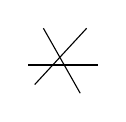
\begin{tikzpicture}[scale=0.55]
\draw (-0.8,0)--(0.8,0);
\draw (-0.65,-0.45)--(0.55,0.85);
\draw (-0.45,0.85)--(0.4,-0.65);
\end{tikzpicture}
\end{adjustbox}

Есть конфигур. теоремы (Паппа, Дезарга, Паскаля и т.д.)

Можно ли выпрямить реш. общего ур-я?

Линейное место $\Longrightarrow$ верны все конфиг. теор. (Дезарга или синусоид).
\begin{equation*}
y''+a(x)y'+b(x)y=0
\end{equation*}
прив. диффеом. плоскости $(x,y)$, линейным по $y$:
\begin{equation*}
x=f(\tilde x),\qquad y=g(\tilde x)\tilde y.
\end{equation*}
Локально приводится к $y''=0$.

\SourcePage{GELFAND-P000665}{unlabelled}
Рассм. произвольное сем-во.

Инфинитезимальная теория небезызвестна.

\underline{E. Cartan} в 1924–25 г., — проективная связность —

— решения — геодезич. эт. этой связности.

Проект. связность — связн. в $G$-рассл., где $G$ — проект. группа,
действ. в кас. пр-ве.

Пр-во линейных элементов $(x,y,y')$.

2) В $\mathbb R^3$ есть 2 сем. повр.

[Справа:]
\begin{adjustbox}{max width=\linewidth}
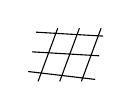
\begin{tikzpicture}[scale=0.5]
\draw (-0.1,0)--(1.6,-0.2);
\draw (0,0.5)--(1.7,0.4);
\draw (0.1,1)--(1.8,0.9);
\draw (0.15,-0.25)--(0.65,1.1);
\draw (0.7,-0.25)--(1.2,1.1);
\draw (1.25,-0.25)--(1.75,1.1);
\end{tikzpicture}
\end{adjustbox}

Гр. диффеом. $\mathbb R^3$ действует.

[Перед вопросом густо наведён отдельный знак.]
\Unclear{GELFAND-P000665}{question-prefix}{Отдельный густо наведённый знак перед К не установлен.}
К какому виду можно привести?

\underline{Эти задачи эквивалентны.}

Выбр. 1 пов., сужаем. всё на плоскость. Там
\Unclear{GELFAND-P000665}{restriction-word}{Слово после «Выбр. 1 пов.»: сужаем.?}
2-коорд. сем-ва и т.д.

В жизни \underline{Бляшке} занимался.

В $\mathbb R^3$ есть контактная структура. (плоскости, натян. на кас. векторы).

Кривые эт. структ. локально проективной прямой.

(из общей теории многомерных расслоений)

На окружности есть много не-эквив. структур проект. пр-ва,

1) $\mathbb {RP}^1$; 2) $S^1\to\mathbb {RP}^1$ [под стрелкой: степ. 2].

2) не-эквив. структуры.

\underline{Д-во не-эквив.:} просим. вект. поля (инфинитезим. автом. этой структуры).

на $\mathbb {RP}^1$ $\frac{\partial}{\partial x}$, $x\frac{\partial}{\partial x}$, $x^2\frac{\partial}{\partial x}$.

\underline{Задача:} как [зачёркнута запись]
\Incomplete{GELFAND-P000665}{cancel-first}{Зачёркнутое слово между «как» и «уравнение» не читается полностью.}
уравнение [зачёркнута запись]
\Incomplete{GELFAND-P000665}{cancel-second}{Зачёркнутое слово после «уравнение» не читается полностью.}
в многом. проектив-ное пр-во?
\Unclear{GELFAND-P000665}{question-word}{Сокращённое слово перед «проектив-ное»: многом.?}

Примем одну реш. за прямую [справа:]
\begin{adjustbox}{max width=\linewidth}
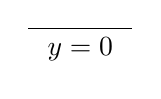
\begin{tikzpicture}[scale=0.55]
\draw (0,0)--(2.4,0);
\node[below] at (1.2,0) {$y=0$};
\end{tikzpicture}
\end{adjustbox}
\begin{equation*}
y''=a(x)y+b(x)p+\ldots
\end{equation*}
[Справа: лин. все. степ. по $y'$.]
\begin{equation*}
p=y'.
\end{equation*}
Выпрямляем лин. ур-е выбор. $x$ сопр. с т-ми её проективного пр-ва.
\begin{equation*}
\begin{cases}\tilde x=f(x),\\\tilde y=g(x)y.\end{cases}
\end{equation*}
($f$ уд. ур-ю типа Шварца).

\SourcePage{GELFAND-P000666}{unlabelled}
Отсюда на $\forall$ реш. возникает проект. структура.

Теперь нач. с квадр. части.
\begin{equation*}
y''=a(x)y^2+b(x)yy'+c(x)y'^2+\ldots
\end{equation*}
[Снизу выделен дугой член $a(x)y^2$; скобкой — следующие два члена.]

Теперь диффеом. плоскости всей.
\begin{equation*}
\begin{cases}\tilde x=x+yf(x,y),\\\tilde y=y(1+yg(x,y)).\end{cases}
\end{equation*}
Убьём $b$ и $c$ этими диффеом.

Останется $a$, опр. с точн. до мультипл. постоянной.
\begin{equation*}
\underline{a(x)(dx)^{5/2}}\quad\text{— опр. с точн. до мульт. постоянной.}
\end{equation*}
Это $5/2$-форма вдоль решения, опр. с точн. до мульт. конст., зав. от решения.

\underline{Теорема.} Если $a(x)(dx)^{5/2}\equiv0$, то ур-е выпрямляемо.

(в форм. рядах)

Дальнейшие дифф-мы прив. к $y''=y'^2A(x,y,y')$.

Рассм. ур-е вида $y''=P_3(y')$ — многоч. 3-й степени отн. $y'$.

Этот класс инвар. отн. диффеоморфизмов.

Появл. этих ур-ий отмеч. \underline{R. Liouville}.

\underline{Скалярный инвариант.}

Извест. форма $\forall$ друг. степ. (в частн. вект. поле)
\begin{equation*}
v(x)=(a(x))^{-2/5}\frac{\partial}{\partial x}.
\end{equation*}
[Формула охвачена скобкой снизу.]

Скаляр устроим теперь: хотим, такую конструкц. с действ. проект. группы.
Получим инварианты:

$I_2,I_3,\ldots$ — инварианты.

Рассм. 2-струю поля. На 2-струях проект. гр. действ. присоед. представлением.
\begin{equation*}
I_2=2v''v-v'^2,
\end{equation*}
\begin{equation*}
I_3=vI_2',\qquad\text{— — —}
\end{equation*}
\begin{equation*}
I_n=vI_{n-1}'.
\end{equation*}
\underline{Гип. Гельфанда:} связано с когомологиями Гельфанда–Фукса.

\underline{Pommaret} занимался дифф. инвариантами.

\SourcePage{GELFAND-P000667}{unlabelled}
\underline{20/IX-76 г. Сем. Гельфанда.}

\underline{С.П. Новиков. Супералгебры в физике.}

[Зачёркнуто: Обз.?]
\Unclear{GELFAND-P000667}{cancel-review}{Зачёркнутое начало перед «Обзор»: Обз.?}
Обзор Огиевецкого в УФН и обзор Зумино.

[На правом поле: \underline{Волков, Акулов}. Слева от этих имён заштрихованный вертикальный прямоугольник.]

Супералгебра [зачёркнуто: Ли?]
\Unclear{GELFAND-P000667}{cancel-super}{Короткая густо зачёркнутая запись после «Супералгебра»: Ли?}
— прям. сумма $L=L_{\text{чет}}\oplus L_{\text{нечет}}=L_0\oplus L_1$.

$[a,b]$ опр. структ. градуир. алгебры Ли.
\begin{equation*}
[a,b]=(-1)^{da\cdot db+1}[b,a],\qquad da=\dim a.
\end{equation*}
Тожд. Якоби тоже вып. со знаками.

Пусть $L_0$ и $L_1$ влож. в ассоц. алгебру (напр., матриц).

$L$ — подалгебра матр. алг., замкн. отн. операции
\begin{equation*}
1)\quad a,b\in L_0\ \Longrightarrow\ ab-ba=[a,b]\in L_0,
\end{equation*}
\begin{equation*}
2)\quad a,b\in L_1\ \Longrightarrow\ ab+ba=[a,b]\in L_0.
\end{equation*}

\SourcePage{GELFAND-P000668}{unlabelled}
\begin{equation*}
3)\quad a\in L_0,\ b\in L_1\ \Longrightarrow\ ab-ba=[a,b]\subset L_1.
\end{equation*}
Или
\begin{equation*}
[a,b]=(-1)^{\varepsilon_1\varepsilon_2+1}[b,a],\qquad
\varepsilon_1=\operatorname{deg} a,\quad\varepsilon_2=\operatorname{deg} b.
\end{equation*}
Впервые рассм. в раб. Гельфанда и Лихтмана конкр. супералгебры.
\begin{equation*}
\mu=0,1,2,3.
\end{equation*}
Всё в $\mathbb R^4$ Минковский.
\begin{equation*}
\eta_{\nu,\mu}=\begin{pmatrix}-1&&&0\\&1&&\\&&1&\\0&&&1\end{pmatrix}
\quad\text{— метрика.}
\end{equation*}
Пр-во спиноров — 4-мерное пр-во [вставлено над «пр-во»: веществ.; ниже зачёркнута запись]
\Incomplete{GELFAND-P000668}{cancel-complex}{Зачёркнутое слово в обведённой вставке о пр-ве спиноров не читается полностью.}
(с базисом) $G_j$, $j=1,2,3,4$.
\begin{equation*}
\alpha=\sum\alpha^jG_j.
\end{equation*}
Алгебра матриц порожд. матр. $\gamma_\mu$ (вещ.) — базис Майорана.
\begin{equation*}
\gamma_\mu\gamma_\nu+\gamma_\nu\gamma_\mu=2\eta_{\nu\mu}.
\qquad(\approx\text{ кватернионы})
\end{equation*}
Выбрать 4 матрицы $\gamma_\mu$, веществ. и обр. базис Майорана

(см. Ахиезер, Берестецкий).

Положим
\begin{equation*}
\bar G_j=G_j\gamma_0;\qquad\bar\alpha=\alpha\gamma_0.
\end{equation*}
$L_0$ — алг. [зачёркнуто: Пуанкаре] трансляций.

$L_1$ — пр-во спиноров.
\begin{equation*}
1)\quad[L_1,L_0]=0,
\end{equation*}
\begin{equation*}
2)\quad[L_1,L_1]\text{ — ?}
\end{equation*}
\begin{equation*}
[\bar G_i,\bar G_j]=-2(\gamma^\mu)_{ij}P_\mu.
\end{equation*}
$P_\mu$ — опер. трансляции Пуанкаре, $\mu$ — индекс.

\underline{Г. Задача:} расширить алг. Пуанкаре до супералгебры.

$A$ — скал. поле;

$B$ — псевдоскал. поле;

$\psi$ — спин. поле;

$F$ — —»—;

$G$ — псевдоск. поле.

[Слева $F$ и $G$ объединены скобкой: вспом. поля. Справа вдоль $A,B,\psi,F,G$ вертикальная линия, к ней направлена стрелка от подписи «супермультиплет».]
\begin{equation*}
\begin{aligned}
L={}&-\frac12\bigl((\partial_\nu A)^2+(\partial_\mu B)^2+i\bar\psi\gamma^\mu\partial_\mu\psi+{}\\
&{}+m^2A^2+m^2B^2+im\bar\psi\psi\bigr)
+gmA(A^2+B^2)-\frac{g^2}{2}(A^2+B^2)^2-{}\\
&{}-ig\,[im\text{ зачёркнуто?}]\,\bar\psi(A-\gamma_5B)\psi.
\end{aligned}
\end{equation*}
\Unclear{GELFAND-P000668}{cancel-term}{Зачёркнутые знаки после «−ig» перед ψ с чертой: im?}

[Внизу зачёркнута запись в скобках, читается начало: суперсимм. лагран…]
\Incomplete{GELFAND-P000668}{cancel-bottom}{Конец зачёркнутой записи в скобках внизу не читается полностью.}
\SourcePage{GELFAND-P000669}{unlabelled}
Опер. из $L_0$ и $L_1$ действуют на лагранжиан $L$ (строится предст.)
и он инвариантен.

\underline{Суперсимм. лагранжиан Вейсса-Зумино.}
\begin{align*}
L={}&-\frac12\bigl((\partial_\nu A)^2+(\partial_\mu B)^2
+i\bar\Psi\,\gamma^\beta\,\partial_\mu\Psi-F^2-G^2\bigr]+{}\\
&+m(FA+GB-i\bar\Psi\Psi)
+g(FA^2-FB^2+2GAB-i\bar\Psi\Psi A+i\bar\Psi\gamma_5\Psi B).
\end{align*}
\Unclear{GELFAND-P000669}{lagrangian-index}{[В этом члене у $\gamma$ верхний индекс $\beta$, у $\partial$ нижний $\mu$.]}
\Unclear{GELFAND-P000669}{lagrangian-brackets}{[Внешняя открывающая скобка круглая, закрывающая квадратная.]}

По $F$ и $G$ нет дифф. $\Rightarrow$ из ур-й Эйлера они исключаются $\Rightarrow$

$\Rightarrow$ предыд. лагран-жиан.

\underline{Действие суперобращениях.}
\begin{gather*}
L=L_0+L_1.\\
\alpha\in L_1,\quad \alpha=\sum\alpha_jQ_j,\qquad \bar\alpha=\alpha\gamma_0.
\end{gather*}
1) $[\bar\alpha,A]=\delta A=i\bar\alpha\Psi;$

2) $\delta B=$ [зачёркнуто: \Unclear{GELFAND-P000669}{delta-b-cancel}{неразборчивое выражение}] $i\bar\alpha\gamma_5\Psi;$

3) $\delta\Psi=\partial_\mu(A-\gamma_5B)\gamma^\mu\alpha+(F+\gamma_5G)\alpha;$

4) $\delta F=i\bar\alpha\gamma^\mu\partial_\mu\Psi;$

5) $\delta G=i\bar\alpha\gamma_5\gamma^\mu\partial_\mu\Psi.$

\underline{\underline{Мигдал (Саша).}} \underline{О калибровочных полях.}

Возникли из попытки описать экспер. данные (о нуклонах).
Они говорят, что нуклоны состоят из \underline{кварков}.

$p\sim$ \begin{adjustbox}{max width=\linewidth}

\begin{tikzpicture}[baseline=-0.12cm]
\draw (0,0) circle (0.34);
\fill (0,0.21) circle (0.055);
\fill (-0.17,-0.12) circle (0.055);
\fill (0.17,-0.12) circle (0.055);
\end{tikzpicture}
\end{adjustbox} (3 кварка).
Внутри свободны, а вынуть их невозможно.

[Зачёркнуто: Они.] \underline{Кварки видны} — просвечивание
[вставлено над строкой, обведено: протона] $\gamma$-квантами
(как в целлофановом мешке).

\underline{В теории силы должны расти с расстояниями!}

[Зачёркнуто: \Unclear{GELFAND-P000669}{principle-cancel}{неразборчивое слово}]
По принципу неопр. они не могут слиться.

\underline{Релятив. инвар.} мешает зад. закон сил (потенциал взаимод. —
вещь релятив. неинвар.)

\underline{Локальность} проверена просвечиванием — кварки почти точечны.

надо строить лагранжианы.

Такой зак. сил даёт калибр. теория.

\underline{Кварк} — \underline{матрица}
\begin{adjustbox}{max width=\linewidth}
\begin{tikzpicture}[x=1cm,y=1cm,baseline=(mat.center)]
\node (mat) at (2.4,1.8) {$\begin{pmatrix}p_1&n_1&\lambda_1\\p_2&n_2&\lambda_2\\p_3&n_3&\lambda_3\end{pmatrix}$};
\node at (0.65,2.0) {$G$};
\draw[->] (0.92,2.32) -- (0.92,1.79);
\draw (0.57,1.30) -- (0.74,1.57);
\draw (0.61,1.28) -- (0.78,1.55);
\node at (0.45,0.94) {$SU(3)$};
\node at (0.45,0.52) {(цветовая)};
\draw[->] (1.45,1.01) -- (3.00,1.01);
\draw[->] (1.76,0.50) -- (1.94,0.82);
\node at (2.48,0.19) {гр. неизвестна.};
\node at (5.05,2.04) {гр. \underline{цвета}};
\node at (5.05,1.59) {и гр. \underline{запаха}.};
\end{tikzpicture}
\end{adjustbox}

Кварков 9 штук.

Силы, не позв. разрушиться, связаны с цветом.

\underline{Цветной гр.} отвеч. [зачёркнуто: \Unclear{GELFAND-P000669}{color-cancel}{неразборчивый знак}]
гораздо более сильная симм. — \underline{калибровочная}.

Мезоны постр. из \underline{кварка и антикварка}.

\SourcePage{GELFAND-P000670}{unlabelled}
\underline{18/X-76.} \underline{Сем. Гельфанда.}

[Зачёркнуто: \Incomplete{GELFAND-P000670}{top-cancel}{Содержание целиком зачёркнутой строки не удалось прочитать.}]
\underline{Написать основные понятия и уравнения, которые надо знать.}
\underline{И задачи.}

\underline{\underline{Задача}}: записать
\Unclear{GELFAND-P000670}{factor-type}{$\mathrm{II}_1$; нижний индекс густо обведён}-факторы
через матрицы непр. порядка.

(не бесплатная)

\underline{\underline{И. Бернштейн.}} (\underline{продолжение}).

\underline{Суперпространство} — неформально: есть 2 группы перем.
\begin{gather*}
\Vert\quad x_1,\ldots,x_p,\\
\phantom{\Vert\quad}\xi_1,\ldots,\xi_q
\end{gather*}

\underline{Формально}
\begin{gather*}
C^\infty(\mathbb R^p)\otimes\Lambda(\xi_1,\quad,\xi_q)
\end{gather*}
Элемент:
\begin{gather*}
\sum f_{\alpha_1.\quad\alpha_q}(x)\xi_1^{\alpha_1}\cdots
\xi_q^{\alpha_k},
\qquad \alpha_i=0,1.
\end{gather*}
\Unclear{GELFAND-P000670}{last-exponent}{[У последнего $\xi_q$ показатель записан как $\alpha_k$.]}
Все $f$ коммутир. с $\xi$, и $\xi_i\xi_j=-\xi_j\xi_i$, $\xi_i^2=0$.

$\mathbb Z_2$ — \underline{Градуировка}.
\underline{Степень} — сумма $\alpha_i\bmod 2$. $\Vert$

\underline{\underline{Другое опред.}}
[Зачёркнуто: \Unclear{GELFAND-P000670}{ringed-cancel}{неразборчивый знак}]
\underline{Кольцованное пр-во}.

$\mathbb R^p$ на нём пучок
\Unclear{GELFAND-P000670}{sheaf-letter}{$\mathcal A_{p,q}$ или $\alpha_{p,q}$}.
\begin{gather*}
U\subset\mathbb R^p\quad\longmapsto\quad\text{кольцо }C^\infty(U)\otimes\Lambda(\xi_1,\ldots,\xi_q),\\
U\subset V\quad\Rightarrow\quad\text{есть естеств. отобр. ограничения}.
\end{gather*}

\underline{\underline{Суперобласть.}} Это топологич. пр-во $U\subset\mathbb R^p$ с тем же пучком
\begin{gather*}
U=(U,\text{\Unclear{GELFAND-P000670}{sheaf-letter}{$\mathcal A_{p,q}$ или $\alpha_{p,q}$}}).
\end{gather*}

[Зачёркнуто над следующим заголовком: \Unclear{GELFAND-P000670}{example-cancel}{неразборчивое слово}]

\underline{Пример.} $u,\xi_1,\xi_2$, $0<u<1$.

\begin{adjustbox}{max width=\linewidth}
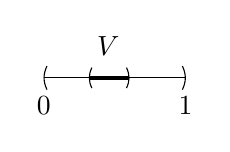
\begin{tikzpicture}[x=1cm,y=1cm,baseline=-0.1cm]
\draw (0,0)--(1.8,0);
\draw (0.04,0.15) to[bend right=25] (0.04,-0.15);
\draw (1.76,0.15) to[bend left=25] (1.76,-0.15);
\draw[line width=1.2pt] (0.58,0)--(1.08,0);
\draw (0.61,0.13) to[bend right=25] (0.61,-0.13);
\draw (1.05,0.13) to[bend left=25] (1.05,-0.13);
\node at (0.82,0.4) {$V$};
\node at (0,-0.35) {$0$};
\node at (1.8,-0.35) {$1$};
\end{tikzpicture}
\end{adjustbox}

Функции на $V=C^\infty(V)\otimes\Lambda(\xi_1,\xi_2)$.
\begin{gather*}
f_{00}(u)+\text{[зачёркнуто: \Unclear{GELFAND-P000670}{function-cancel}{неразборчивая группа знаков}]}
f_{10}(u)\xi_1+f_{01}\xi_2+f_{11}(u)\xi_1\xi_2.
\end{gather*}

$C^\infty(\widetilde U)$ — обозначение для пр-ва ф-й на суперобласти $\widetilde U$.
\begin{gather*}
C^\infty(\widetilde U)=C^\infty(U)\otimes\Lambda(\xi_1,\ldots,\xi_q).
\end{gather*}

\underline{Отображение суперобластей} $\varphi:\widetilde U\longrightarrow\widetilde V$
это набор объектов: \underline{отображение} $\varphi':U\longrightarrow V$
и \underline{отобр.}
\begin{gather*}
C^\infty(\widetilde V)\longrightarrow C^\infty(\widetilde U),
\end{gather*}
гом. колец, накрывающий $\varphi'$ (с единицей) и сохр. \underline{чётность}!!

[Слева зачёркнуто: \Unclear{GELFAND-P000670}{map-cancel}{и если $V\supset V_0$; знак между $V$ и $V_0$ неясен}.]

\underline{\underline{Пример:}}
\begin{adjustbox}{max width=\linewidth}
\begin{tikzpicture}[x=1cm,y=1cm,baseline=-0.08cm]
\node at (0,0) {$U$};
\fill (0.90,0) circle (0.035);
\node at (1.46,0.33) {$1$};
\node at (2.28,0) {$\xi_1,\xi_2$};
\end{tikzpicture}
\end{adjustbox}

\underline{$p=0,\ q=2$.}
Суперобл. размерности $(0,2)$.

Геометрически — точка.
отобр. суперобл. в себя — эндоморфизм.

кольцо $\Lambda(\xi_1,\xi_2)$.
\begin{gather*}
1\longmapsto1,\\
\xi_1\longmapsto a\xi_1+b\xi_2+c\,\text{[зачёркнуто: $\xi_1\xi_2$]},\\
\xi_2\longmapsto a'\xi_1+b'\xi_2+c'\,\text{[зачёркнуто: $\xi_1\xi_2$]}.
\end{gather*}
[Справа, со стрелкой к зачёркнутому произведению:] нельзя, т.к. сохр. чётность.

\underline{\underline{$a,b,a',b'$}} — любые.

\SourcePage{GELFAND-P000671}{unlabelled}
\underline{Алгебра} $\Lambda(\xi_1,\xi_2)$ \underline{коммутативна в суперсмысле.}
\begin{equation*}
xy=(-1)^{p(x)p(y)}yx.
\end{equation*}

\underline{Пример 2.}
\begin{equation*}
\begin{array}{l}
u,\xi_1,\xi_2\\
v,\eta_1,\eta_2
\end{array}
\qquad
\left\Vert\begin{aligned}
v&=u+\xi_1\xi_2\\
\eta_1&=\xi_1\\
\eta_2&=\xi_2.
\end{aligned}\right.
\end{equation*}

\underline{Задача:} куда переходит $\sin v$?

Элемент кольца левого им. вид
\begin{equation*}
f_{00}(u)+f_{10}(u)\xi_1+f_{01}(u)\xi_2+f_{11}(u)\xi_1\xi_2
\end{equation*}
Элем. 2-го кольца
\begin{equation*}
g_{00}(v)+g_{10}(v)\xi_1+g_{01}(v)\xi_2+g_{11}(v)\xi_1\xi_2
\end{equation*}

\underline{отобр.}
\begin{gather*}
\widetilde U\longrightarrow\widetilde V\\
C^\infty(\widetilde V)\longrightarrow C^\infty(\widetilde U)\\
g_{00}(v)\mapsto g_{00}(u+\xi_1\xi_2)=g_{00}(u)+\xi_1\xi_2g'_{00}(u).
\end{gather*}

$x=(u_1,\ldots,u_p,\xi_1,\ldots,\xi_q)$ — система координат.
\begin{equation*}
\frac{\partial}{\partial u_i}f\xi_1^{\alpha_1}\ldots\xi_q^{\alpha_q}
=\frac{\partial f}{\partial u_i}\xi_1^{\alpha_1}\ldots\xi_q^{\alpha_q}
\end{equation*}

\underline{Теорема Стокса — ?}

Интеграл суперфункции по суперобласти.

\underline{Аналог в обычном анализе}

\SourceFigure{GELFAND-P000671}{oval-diagram}{Неподписанный наклонный овал; внутри проведена восходящая слева направо линия, пересечённая короткими штрихами.}
\Unclear{GELFAND-P000671}{middle-phrase}{структ. в опр. подмногообразиях — чтение неуверенное}

Интеграл для ф-й на мн-ии с границей неинвар.
от. замен переменных.

Отличие: здесь интегрировать формы нельзя. Можно плотности
(при замене коорд. умн. на \underline{Березиниан})

\underline{\underline{Что интегр. по границе?}}

$\underline{\underline{U,\partial U.}}$
\quad $f=0$, где $f\in C^\infty(U)$ — \underline{суперфункция.}

\underline{Замкн суперобласть.}
\quad $\underline{\underline{u,\xi_1,\xi_2}}$

$\uparrow$ замкн. обл. с гладк. гр. $\partial U$.

На $\partial U$ есть структ.
\Unclear{GELFAND-P000671}{lower-supermanifold}{супермн-зия; над строкой вставлено «под»}

($\overset{\text{чётным}}{\underline{\text{ур-ем}}}$
\Unclear{GELFAND-P000671}{lower-cancellation}{зачёркнуто, неразборчиво}
\underline{выделяется})

$\underline{\underline{[0,\infty)}}$
\qquad $\underline{\underline{u,\xi_1,\xi_2.}}$

Разные суперобласти

1. $u=0$

2. $u+c\xi_1\xi_2=0$

\SourceFigure{GELFAND-P000671}{bottom-diagram}{Узкий наклонный четырёхугольник с тёмными продольными штрихами внутри, без подписей.}
\underline{чётное ур-е}

\SourcePage{GELFAND-P000672}{unlabelled}
\underline{\underline{Подмн-зие:}} в кольце выб. идеал ф-и.

Граница — \underline{чётная.}

$C^\infty(\widetilde U)$ \qquad граница — \underline{ур-е} $\underline{\underline{f(\widetilde U)=0}}$

\begin{equation*}
\int\text{финитной ф-и}=\int f_{11\ldots1}\,du_1\ldots du_p
\end{equation*}

\underline{Для замкн. областей иначе.}

Пусть полупр-во $\underline{\underline{u_1\ge0}}$

Тогда интегр. зад. такой же ф-лой.

Он сохр., если перех. в себя как супермн-зие.

\begin{adjustbox}{max width=\linewidth}

\begin{tikzpicture}[scale=0.55]
\draw (0,0) circle (0.7);
\draw (-0.56,-0.15) -- (-0.18,0.55);
\draw (-0.40,-0.40) -- (0.03,0.52);
\draw (-0.13,-0.42) -- (0.27,0.35);
\draw (0.12,-0.38) -- (0.46,0.22);
\draw (0.37,-0.34) -- (0.59,0.04);
\end{tikzpicture}
\end{adjustbox}
$u_1^2+u_2^2\le1$
\begin{gather*}
u_1^2+u_2^2-1=0\quad(1)\quad\text{— 2 границы}\\
u_1^2+u_2^2-1-\xi_1\xi_2=0\quad(2)
\end{gather*}

Интеграл по обл. с границей (2):
\begin{equation*}
\int[f_{00}(u)+f_{01}(\ )\xi_1+\ldots]
\end{equation*}

\underline{Грубо}
\begin{equation*}
\int\xi_1\xi_2\,d\xi_1\,d\xi_2=1
\end{equation*}

— Для обычной границы —
\begin{equation*}
\int_{u_1^2+u_2^2<1}f_{11}(u)\,du_1du_2
\end{equation*}

\underline{Проверка инвариантности} — надо, чтобы ур-е гран. ост. старым.

Если граница $\underline{u_1^2+u_2^2-1-\xi_1\xi_2=0}$

надо сделать зам. пер., чтобы гран. перешла в нормальную
\begin{equation*}
\underline{\left(u_1-\frac12\xi_1\xi_2\right)^2+u_2^2-1=0.}
\end{equation*}

\Unclear{GELFAND-P000672}{upper-cancellation}{зачёркнуто: u=0 — чтение неуверенное}

\begin{adjustbox}{max width=\linewidth}
\begin{tikzpicture}[scale=0.6]
\draw (0,0) -- (3.5,0);
\draw (0,-0.16) -- (0,0.16);
\node[below] at (0,0) {$0$};
\node[below] at (3.5,0) {$\infty$};
\end{tikzpicture}
\end{adjustbox}
\begin{equation*}
\int_0^\infty f_{11}(u)\,du\qquad u,\xi_1,\xi_2
\end{equation*}
гран. $u=0$.

$\underline{v=u+u\xi_1\xi_2.}$

Будет граница $\underline{\underline{v=0}}$

\begin{multline*}
\int_0^\infty g_{11}(v)\,dv
=\int_0^\infty g_{11}(u+u\xi_1\xi_2)\,dv
=\int_0^\infty g_{11}(u)\,dv\\
+\int_0^\infty g'_{11}(u)u\xi_1\xi_2\,dv
\end{multline*}

\SourceFigure{GELFAND-P000672}{integral-sketch}{Под длинной формулой — открытая кривая, нисходящая вправо, с несколькими длинными косыми штрихами и петлеобразными пересечениями; подписей нет.}
\begin{equation*}
\frac{Dv}{Du}
\end{equation*}

\underline{Интеграл по обл. с границей —}

\underline{— Бернштейн и Лейтес}

\Unclear{GELFAND-P000672}{lower-cancellation}{зачёркнуто, неразборчиво}

Есть раб. \underline{Березина} и Маринова (?)

\underline{классич. мех. в Ферми и Бозе — переменных}

\underline{Задача:} Теор. Стокса для круга
$u_1^2+u_2^2+c\xi_1\xi_2-1=0$

\SourcePage{GELFAND-P000673}{unlabelled}
\underline{Конспект предыдущих супердокладов И. Бернштейна}

\underline{(по тетради \Unclear{GELFAND-P000673}{notebook-author}{Н. Зорина — чтение неуверенное})}

\underline{Опред.} \underline{Суперкольцо}
\begin{equation*}
A=\underset{\text{чётн}}{A_0}\oplus\underset{\text{нечётн}}{A_1}
\qquad
\begin{aligned}
A_0A_0&\subset A_0\\
A_0A_1&\subset A_1\\
A_1A_0&\subset A_1\\
A_1A_1&\subset A_0
\end{aligned}
\end{equation*}

Оно наз. \underline{коммутативным}, если $\underline{ab=ba(-1)^{\operatorname{deg}a\cdot\operatorname{deg}b}}$

\underline{Линейная алгебра.}

\Unclear{GELFAND-P000673}{cancelled-glyph}{зачёркнутый знак, неразборчиво}
[Над коммут. суперкольцом рассмотрим
\Unclear{GELFAND-P000673}{cancelled-word-one}{зачёркнуто, неразборчиво}
люб. $A$-модуль $A^n$ и
его \Unclear{GELFAND-P000673}{cancelled-word-two}{зачёркнуто, неразборчиво}
эндоморфизм, задаваемый блочной матрицей]

\begin{equation*}
[A=]\begin{pmatrix}A_{11}&A_{12}\\A_{21}&A_{22}\end{pmatrix}
\qquad
\det A\underset{\mathrm{def}}{=}
\det A_{11}^{-1}\det(A_{22}-A_{21}A_{11}^{-1}A_{12})
\end{equation*}

\begin{gather*}
\operatorname{str}A=\operatorname{tr}A_{11}-\operatorname{tr}A_{22}.\\
(\text{суперслед})
\end{gather*}

\underline{Свойства:}
\begin{gather*}
\det XY=\det X\cdot\det Y.\\
\det X=\exp\operatorname{str}\ln X_{\text{\Unclear{GELFAND-P000673}{logarithm-tail}{0, 1 или зачёркнутый знак}}}\\
\operatorname{str}(XY)=\operatorname{str}(YX)\\
\begin{pmatrix}A&B\\C&D\end{pmatrix}^{*}
=\begin{pmatrix}A^{*}&C^{*}\\-B^{*}&D^{*}\end{pmatrix}
\end{gather*}

\underline{Суперанализ.}

Рассм.
\begin{equation*}
\sum f_{i_1\quad i_k}(x_1,\quad x_p)\xi_1^{i_1}\ldots\xi_k^{i_k}
\end{equation*}

Правила диффер.
\begin{gather*}
\frac{\partial}{\partial\xi_1}(\xi_1\xi_2)=\xi_2,\qquad
\frac{\partial}{\partial\xi_2}(\xi_1\xi_2)=-\xi_1,\\
\frac{\partial}{\partial\xi_1}\xi_2=0,\qquad
\frac{\partial}{\partial\xi_1}\xi_1=1,\qquad
\frac{\partial}{\partial\xi_1}1=0.
\end{gather*}

\rule{12cm}{0.4pt}

Рассм. блочные матрицы
$\begin{pmatrix}A&B\\C&D\end{pmatrix}$
\begin{equation*}
A=A_{\bar0}\oplus A_{\bar1}
\qquad
\begin{aligned}
\text{элем. }A,D&\in A_{\bar0}\\
\text{элем. }B,C&\in A_{\bar1}
\end{aligned}
\end{equation*}

$\mathbb Z/2\mathbb Z$ — град.

$\bar0,\bar1$ — элем.

$p(a)$ — чётность.

\begin{gather*}
\operatorname{Ber}J=(\det D)^{-1}\cdot\det(A-BD^{-1}C)\in A_{\bar0}\\
(\text{березиниан})
\end{gather*}

\underline{У-тв}
\begin{gather*}
\operatorname{Ber}J_1J_2=\operatorname{Ber}J_1\cdot\operatorname{Ber}J_2.\\
\operatorname{str}J=\operatorname{tr}A-\operatorname{tr}D
\end{gather*}

\underline{У-тв.}
\begin{equation*}
\operatorname{str}(J_1J_2)=\operatorname{str}(J_2J_1).
\end{equation*}

\rule{12cm}{0.4pt}

В $\mathbb R^p$ рассм. $C^\infty(\mathbb R^p)\otimes\underset{\substack{\uparrow\\\text{внешняя алг.}}}{\Lambda}(\xi_1,\ldots,\xi_q)$

$p(\xi_i)=1,\qquad\xi_i\xi_j=-\xi_j\xi_i.$

\SourcePage{GELFAND-P000674}{unlabelled}
\begin{equation*}
\Lambda(\xi_1,\ldots,\xi_q)\ni\xi_1^{\alpha_1}\cdots\xi_q^{\alpha_q},\qquad \alpha_i=0,1.
\end{equation*}
\begin{equation*}
f=\sum f_{\alpha_1\alpha_2\ldots\alpha_q}\,\xi_1^{\alpha_1}\cdots\xi_q^{\alpha_q}.
\end{equation*}
\underline{Опр.}
\begin{equation*}
\mathbb{R}^{p,q}=(\mathbb{R}^p,C^\infty(\mathbb{R}^p)\otimes\Lambda(\xi_1,\ldots,\xi_q))
\end{equation*}
— суперпр-во разм. $(p,q)$.

\underline{Опр.}
\begin{equation*}
U=\left(u,\underbrace{C^\infty(u)\otimes\Lambda(\xi_1,\ldots,\xi_q)}\right)
\end{equation*}
\underline{суперобласть.}

(кольцеванное пр-во!)

$(\mathrm{def})\ C^\infty(U)$ — кольцо ф-й на \Unclear{GELFAND-P000674}{upper-ring-abbreviation}{сбл.}.

отобр. $\widetilde{\psi}:U\to V$
\Unclear{GELFAND-P000674}{upper-morphism-letter}{[неясный знак]} — морфизм кольцев. пр-в —
это отобр. \Unclear{GELFAND-P000674}{upper-map-cancellation}{[зачёркнуто, неразборчиво]}
$\psi:C^\infty(v)\to C^\infty(u)$.

\underline{Коорд. запись.} Пусть в пр-ве $U$ выбр. набор
$(u_1,\ldots,u_p,\xi_1,\ldots,\xi_q)$

\hspace{2em} — '' — $V$ — '' — $(v_1,\ldots,v_m,\eta_1,\ldots,\eta_n)$.

Оказ., что для задания отобр. $\psi:U\to V$
\Unclear{GELFAND-P000674}{middle-map-cancellation}{[зачёркнуто, неразборчиво]}
дост. задать
\begin{equation*}
v_1^*,\ldots,v_m^*,\eta_1^*,\ldots,\eta_n^*.
\end{equation*}
\underline{Пример.}
\begin{equation*}
\begin{aligned}
v&=u+\xi_1\xi_2,\\
\eta_1&=u\xi_1,\\
\eta_2&=\xi_2.
\end{aligned}
\end{equation*}
\underline{Задача.} Как выглядит $\sin v$?

\underline{Утв.}
\begin{equation*}
\frac{\partial}{\partial u_i}(f\xi^\alpha)=\frac{\partial f}{\partial u_i}\,\xi^\alpha,
\end{equation*}
\begin{equation*}
\frac{\partial}{\partial\xi_j}(f\xi_1^{\alpha_1}\cdots\xi_q^{\alpha_q})
=\alpha_j(-1)^{\alpha_1+\ldots+\alpha_{j-1}}f\xi_1^{\alpha_1}\cdots\widehat{\xi}_j^{\alpha_j}\cdots\xi_q^{\alpha_q}.
\end{equation*}

\begin{center}
\rule{2cm}{0.3pt}\quad$\cdot$\quad\rule{2cm}{0.3pt}
\end{center}

Пусть $U$ — суперобласть
\begin{equation*}
x=(u,\xi),\qquad y=(v,\eta).
\end{equation*}
\begin{equation*}
J=(J_{ij}),\qquad J_{ij}=\frac{\partial y_j}{\partial x_i}.
\end{equation*}
\begin{equation*}
\operatorname{Ber}J\underset{\mathrm{def}}{=}D(y)/D(x).
\end{equation*}
\underline{Опред.} $U$, $x=(u,\xi)$.

Выраж. $\rho=fD(x)$ наз. \underline{формой объема}.
\begin{equation*}
fD(x)=f\left(D(x)/D(y)\right)\cdot D(y).
\end{equation*}
\underline{Определение.}
\begin{equation*}
\int_u fD(x)\underset{\mathrm{def}}{=}\int_u f_{11\ldots1}(u)\,du_1\ldots du_p
\end{equation*}
(интеграл формы объема)

\underline{Теорема (березин)} Это выраж. не зависит от системы координат.

Здесь интеграл от финитной ф-и берется.

\SourcePage{GELFAND-P000675}{unlabelled}
\underline{25/X-76.}\qquad \underline{Сем. Гельфанда.}

\underline{Гельфанд.}
\underline{Что такое связность?} (для 1-курсников и Полякова).

— см. Номидзу; Стернберг; Бишоп и Криттенден; Ландау и Лифшиц.

\underline{Попов.}

\underline{Работа основоположников} (Янг, Миллс — перевод в сб. «Элем. частицы и компенсирующие поля»).

Рассмотрим ур-е Дирака

{\small без массы}
\begin{equation*}
\underline{\gamma^\mu\partial_\mu\Psi=0},\qquad
\Psi=(\Psi_\alpha)
\end{equation*}
— 4-комп. обычн. спинор.

Ур-я Янга-Миллса:
\begin{equation*}
\underline{\partial_\nu F_a^{\mu\nu}+\Unclear{GELFAND-P000675}{upper-ym-constant}{f^a_{ac}}F_b^{\mu\nu}A_\nu^c=0},
\end{equation*}
где
\begin{equation*}
F_{\mu\nu}^a=\partial_\mu A_\nu^a-\partial_\nu A_\mu^a+\frac12 f_{bc}^a(A_\mu^b A_\nu^c-A_\nu^b A_\mu^c)
\end{equation*}
на $\mathbb{R}^4$ рассм. метрика Минковского $g_{\mu\nu}$;
$A_\mu^\alpha$, $a=1,\ldots,\dim G$

($G$ — нек-рая группа; счит. обычно полупростой).

опуск. индексов в ур-и с пом.
\begin{equation*}
K_{ab}=f_{ac}^d f_{bd}^c,
\end{equation*}
где $f_{ac}^d$ — структ. пост. алгебры Ли группы.

\begin{center}
\rule{2cm}{0.3pt}\quad$\cdot$\quad\rule{2cm}{0.3pt}
\end{center}

\underline{Г.} О кварках см. ст. \underline{Зельдовича} в УФН \underline{«Кварки для пешеходов»}.

\begin{center}
\rule{2cm}{0.3pt}\quad$\cdot$\quad\rule{2cm}{0.3pt}
\end{center}

Ур-я Янга-Миллса опис. кварки.

$\mu,\nu=1,\ldots,4$;
\Unclear{GELFAND-P000675}{middle-cancellation}{[зачёркнуто, неразборчиво]}
$F_a^{\mu\nu}$ — тензор со знач. в алгебре Ли.

$A$ — аналог вект. потенциала
\begin{equation*}
\partial_\nu=\partial/\partial x^\nu.
\end{equation*}
$F$ — аналог тензора напр.

\underline{Пример.}
Для $G=U(1)$ получаются ур-я электро-динамики.

\underline{Ур-я:}
\begin{equation*}
\left.
\begin{aligned}
\partial_\mu F^{\mu\nu}&=0\\
F^{\mu\nu}&\underset{\mathrm{def}}{=}\partial_\mu A_\nu-\partial_\nu A_\mu
\end{aligned}
\right\Vert
\end{equation*}
Получ. ур-я Максвелла.

\begin{center}
\rule{2cm}{0.3pt}\quad$\cdot$\quad\rule{2cm}{0.3pt}
\end{center}

\underline{Калибровочные преобразования.}

\underline{В эл. и магн. поле:}
\begin{equation*}
\begin{pmatrix}
0&H_{12}&H_{13}&E_1\\
-H_{12}&0&H_{23}&E_2\\
-H_{13}&-H_{23}&0&E_3\\
-E_1&-E_2&-E_3&0
\end{pmatrix}
=F^{\mu\nu};
\end{equation*}
\underline{2-форма}

\underline{Ур-я Максвелла:}
\begin{equation*}
F^{\mu\nu}=\frac{\partial}{\partial x^\mu}A_\nu-\frac{\partial}{\partial x^\nu}A_\mu.
\end{equation*}
— \underline{тензор} \Unclear{GELFAND-P000675}{lower-tensor-cancellation}{[зачёркнуто, неразборчиво]} \underline{2-го пор.}

Преобразования $A$, не меняющие $F$, наз.
\fbox{градиентными}
\Unclear{GELFAND-P000675}{lower-gradient-cancellation}{[под вставкой зачёркнуто: калибр.]}
преобразованиями
\begin{equation*}
A_\mu\to A_\mu+\partial_\mu\alpha
\end{equation*}

\SourcePage{GELFAND-P000676}{unlabelled}
Пусть $(T_a)$ — базис в алгебре Ли $\mathcal{L}(G)$.

Рассм.
\begin{equation*}
B_\mu=T_a A_\mu^a\quad\text{—}\quad\underline{n\times n\text{ матриц.}}
\end{equation*}
\begin{equation*}
F_{\mu\nu}=T_a F_{\mu\nu}^a\quad\text{— — '' —}.
\end{equation*}
\underline{Калибр. Преобр. на полях матриц:}
\begin{equation*}
B_\mu\to B'_\mu=S^{-1}B^\mu S+S^{-1}\partial_\mu S,
\end{equation*}
\begin{equation*}
F_{\mu\nu}^{\Unclear{GELFAND-P000676}{upper-f-cancellation}{\text{[зачёркнуто]}}}
\to F'_{\mu\nu}=S^{-1}F_{\mu\nu}S,
\end{equation*}
где $S:\mathbb{R}^4\to G$.

Легко пров. в лоб, что ур-я инвар. отн. этих преобразований.

Неизвестные — $A$.

Нелинейность за счет некоммут. группы.

($F$ — кривизна связности)

\underline{Ур-я Янга-Миллса.}

Пусть $(P,M,G)$ — главное расслоение

($M$ — мн-ие

$G$ — группа \Unclear{GELFAND-P000676}{middle-group-cancellation}{[зачёркнуто, неразборчиво]} — произвольная)

на $M$ есть невырожденная метрика $g$.

В главном рассл. связность, заданная формой $\Omega\in\mathcal{L}(G)\otimes\Lambda^1(P)$.

На неё и будет ур-е.

Фиксир. произв. квадр. (невыр.) форма $K$ на алгебре Ли $\mathcal{L}(G)$.

По этим данным строится естеств. метрика на $P$.
\begin{equation*}
h_p(Y_p,Y'_p)=g_{\pi(p)}(d\pi Y_p,d\pi Y'_p)+K(\Omega(Y_p),\Omega(Y'_p)).
\end{equation*}
метрика в общем случае неинвар.

\underline{Кривизна связности.}
\begin{equation*}
\underline{\Phi=H\,d\Omega}\Unclear{GELFAND-P000676}{lower-curvature-punctuation}{,}=d\Omega+\frac12[\Omega,\Omega]
\end{equation*}
$H$ — опер. гориз. части формы, постр. по связности.

\underline{Ур-е Янга-Миллса своб. поля}
\begin{equation*}
\fbox{$H\delta_{\Unclear{GELFAND-P000676}{lower-delta-cancellation}{\text{[зачёркнуто]}}}\varphi=0$}
\end{equation*}
$\delta$ — сопр. оператор по метрике $h$.

Это ур-е на главном рассл., а выше — ур-е на базе. Как их отождествить?

\underline{\Unclear{GELFAND-P000676}{lower-heading}{Оказ.}}
\underline{ур-я не зависят от выбора метрики $K$!}

(на эквивар. гориз. формах опер. $H\circ\delta$ не зависит от метрики;

на любых формах со знач. в векторном пр-ве.

гориз. форма — $\underline{\equiv0}$, если один из векторов вертикален.

Надо док., что $H\delta\Phi$ — эквивар. гориз. форма.

\SourcePage{GELFAND-P000677}{unlabelled}
Рассм. окр. $U\subset$ \Unclear{GELFAND-P000677}{top-base-letter}{$N$} и на ней сделаем тривиализацию \Unclear{GELFAND-P000677}{top-section-symbol}{$\zeta$ [зачёркнутый знак справа внизу неразборчив]} главного рассл. (произв. сечение).

\begin{center}
\Unclear{GELFAND-P000677}{connection-formula}{$\displaystyle \theta=\zeta^{*}\Omega=\underset{\substack{\uparrow\\\text{базис в алг. Ли}}}{T_a}\otimes A^a_{\mu}\,dx^{\mu}$}
\end{center}
\begin{center}
\Unclear{GELFAND-P000677}{curvature-formula}{$\displaystyle \zeta^{*}\Phi=T_a\otimes F^a_{\mu\nu}\,dx^{\mu}\wedge dx^{\nu}.$}
\end{center}

\underline{Проекция ур-я:}
\begin{center}
\Unclear{GELFAND-P000677}{projection-formula}{$\displaystyle \underline{\delta_M(\zeta^{*}\varphi)+*^{-1}[\theta,*\zeta^{*}\Phi]=0.}$}
\end{center}
$\delta_M$ — опер. $\delta$ на базе.

Прямое вычисл. показ., что это то же ур-е.

Это то же ур-е, если на группе есть 2-стор. инв. метрика.

\underline{Здесь есть своб. ур-я Эйнштейна} (\underline{тензор Риччи}$=0$)

$G=$ \underline{аффинные преобр. $R^4$}

(ур-е в рассл. афф. реперов)

На афф. реперах есть 2 состав. связн., индуц. метрикой базы.

На классе картановских связностей, инд. метрик.

\Unclear{GELFAND-P000677}{connection-paragraph-mark}{[густо обведённый знак, похожий на 4]}
Есть единств. связн. \Unclear{GELFAND-P000677}{connection-cancel}{[зачёркнутый знак неразборчив]} $\bar\Omega$ в рассл. афф. реперов, такая что
\begin{equation*}
\text{если}\qquad
\underset{\text{лин.}}{L}\overset{i}{\hookrightarrow}\underset{\text{афф.}}{AL}
\qquad i^{*}\bar\Omega=(\Omega^g,\chi),
\end{equation*}
$\chi$ — форма смещения

(ест. форма со знач. в $R^4$ на рассл. \Unclear{GELFAND-P000677}{shift-insertion}{[зачёркнуто: неразборчиво; снизу вписано и обведено «лин.»]} реперов)

$\Omega^g$ — метрическая связность

\begin{center}
\begin{adjustbox}{max width=\linewidth}
\begin{tikzpicture}
\draw (-2.1,0) -- (-0.3,0);
\fill (0,0) circle (0.04);
\draw (0.3,0) -- (2.3,0);
\end{tikzpicture}
\end{adjustbox}
\end{center}

опр. картановской связности — см. бишоп и криттенден.

на этих связностях $\underline{H\delta\varphi=0}$ — \underline{ур-е Эйнштейна} (1-го пор.-\newline
-ка связности!! — не как для общих полей Янга-Миллса)

Ур-я 2-го пор. — \Unclear{GELFAND-P000677}{consequence-cancel}{[зачёркнутый знак неразборчив]} следствие ур-й 1-го порядка.

\begin{adjustbox}{max width=\linewidth}
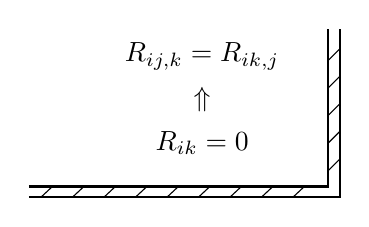
\begin{tikzpicture}
\node at (0,1.45) {$R_{ij,k}=R_{ik,j}$};
\node at (0,0.9) {$\Uparrow$};
\node at (0,0.35) {$R_{ik}=0$};
\draw[line width=0.9pt] (-2.2,-0.2) -- (1.6,-0.2) -- (1.6,1.8);
\draw[line width=0.7pt] (-2.2,-0.34) -- (1.75,-0.34) -- (1.75,1.8);
\draw (-2.05,-0.34) -- (-1.9,-0.2) (-1.65,-0.34) -- (-1.5,-0.2) (-1.25,-0.34) -- (-1.1,-0.2) (-0.85,-0.34) -- (-0.7,-0.2) (-0.45,-0.34) -- (-0.3,-0.2) (-0.05,-0.34) -- (0.1,-0.2) (0.35,-0.34) -- (0.5,-0.2) (0.75,-0.34) -- (0.9,-0.2) (1.15,-0.34) -- (1.3,-0.2);
\draw (1.6,0) -- (1.75,0.15) (1.6,0.35) -- (1.75,0.5) (1.6,0.7) -- (1.75,0.85) (1.6,1.05) -- (1.75,1.2) (1.6,1.4) -- (1.75,1.55);
\end{tikzpicture}
\end{adjustbox}

\SourcePage{GELFAND-P000678}{unlabelled}
\underline{Сем. Гельфанда.}

\underline{И. Н. Бернштейн.}

\underline{Костант.}

\begin{center}
\Unclear{GELFAND-P000678}{euler-product}{$\displaystyle \underline{\varphi(x)=\prod_{n=1}^{\infty}(1-x^n)=(1-x)(1-x^2)(1-x^3)\times\ldots}=\sum_{n=-\infty}^{\infty}(-1)^n x^{(3n^2+n)/2}.$}
\end{center}
\begin{flushright}
$\nearrow$\newline
\underline{Эйлер.}
\end{flushright}

\underline{Якоби:}
\begin{equation*}
\varphi(x)^3=\sum_{n=0}^{\infty}(-1)^n(2n+1)x^{n(n+1)/2}
\end{equation*}
(из \Unclear{GELFAND-P000678}{jacobi-theta-case}{$\Theta$ / $\theta$}-функции).

С тех пор найдены другие (Дайсон и др.)

\underline{Макдональд нашёл групп. основу.}

Легко пров., что
\begin{equation*}
\varphi(x)^{-1}=\sum p(n)x^n,
\end{equation*}
$p(n)$ — число разб. числа $n$ в сумму неотриц. слагаемых

\begin{equation*}
x\varphi(x)^{24}=\sum\tau(n)x^n,
\end{equation*}
$\tau(n)$ — ф-я Рамануджана

это её определение

У $\tau(n)$ есть комбинат. определение

\Unclear{GELFAND-P000678}{dedekind-cancel}{[зачёркнутое слово неразборчиво]}

(через \Unclear{GELFAND-P000678}{dedekind-theta-case}{$\Theta$ / $\theta$}-ф-ю Дедекинда)

можно написать
\begin{equation*}
\varphi(x)^k,\quad\text{где }k\text{ — размерность группы Ли (полупростой)}
\end{equation*}

\begin{equation*}
\begin{array}{cc||}
\varphi^3&SU(2)\\
\varphi^{24}&SU(5)\\
\varphi^{10}&Sp(4)
\end{array}
\qquad
\underline{\text{Макдональд}}\text{: явно выпис. ф-лу}
\end{equation*}
% В источнике фамилия «Макдональд» подчёркнута прерывистой линией.
% Под таблицей идёт линия, которая ступенью поднимается к верхней границе следующего абзаца.
\begin{adjustbox}{max width=\linewidth}
\begin{tikzpicture}
\draw (0,0) -- (3.4,0) -- (3.4,0.65) -- (10.8,0.65);
\end{tikzpicture}
\end{adjustbox}

Пусть есть комп. полупростая группа \Unclear{GELFAND-P000678}{group-cancellations}{[две зачёркнутые группы знаков неразборчивы]} $G$

$g$ — её алгебра Ли, на $g$ есть форма Киллинга $B$

$\Delta$ — оператор Лапласа на \Unclear{GELFAND-P000678}{laplace-cancellations}{[два зачёркнутых фрагмента неразборчивы]} $G$

$X_1,\ldots,X_k$ — ортонорм. базис в $g$.

В обёрт. $\underset{\text{[вписано снизу, обведено: }U(g)\text{]}}{\text{алгебре}}$ рассм. элемент \Unclear{GELFAND-P000678}{enveloping-cancel}{[зачёркнутая формула неразборчива]} $\Delta=\sum X_i^2$,

он 2-стор. инвариантен.
\SourcePage{GELFAND-P000679}{unlabelled}

\begin{equation*}
\varphi(x)^k=
\sum_{\text{непр. предст. }V}
c_V\cdot\dim V\cdot x^{\left.\Delta\right|_V}
\end{equation*}
[В показателе степени перед $\left.\Delta\right|_V$ зачёркнуто:
\Unclear{GELFAND-P000679}{top-exponent-cancellation}{неразборчиво}.]

($\left.\Delta\right|_V$
[Вставлено над строкой с выносом: на непр. предст.]
кратен единичному; соб. значение $\left.\Delta\right|_V$.

[Зачёркнуто:
\Unclear{GELFAND-P000679}{top-word-cancellation}{отсюда}.]
Асимптотика зав. от размерности.

Группы быв. разные и ф-лы тоже.

\begin{equation*}
c_V=\chi_V(a),\quad\text{где }a\in G
\end{equation*}
[Под $a\in G$:] некий элемент.

[Зачёркнуто: Для серии.]
Для $SU(n)$ есть единств. регул. элемент.
(класс сопр. элементов;), т.е. такой, что соб. знач. различны и
[Зачёркнуто:
\Unclear{GELFAND-P000679}{su-n-power-cancellation}{неразборчивый знак}.]
$n$-я степень скалярна

[Слева перед матрицей зачёркнуто:
\Unclear{GELFAND-P000679}{matrix-left-cancellation}{неразборчивый знак}.]
\begin{equation*}
\begin{pmatrix}
\xi&&&&0\\
&\xi^2&&&\\
&&\xi^3&&\\
&&&\ddots&\\
0&&&&\xi^n
\end{pmatrix}c,\qquad
c\quad\underline{\text{подобр., чтобы }\det=1.}
\end{equation*}

Рассм. $\zeta$-функцию опер. Лапласа

\underline{В. Кац} — док-во \underline{через}
$\underline{\infty}$-мерные алгебры Ли.

Рассм.
$-\Delta+\dfrac{\dim\Unclear{GELFAND-P000679}{dimension-letter}{\mathcal G}}{24}$
и положим

\begin{equation*}
\zeta(s)\underset{\mathrm{def}}{=}
\left.\left(-\Delta+
\frac{\dim\Unclear{GELFAND-P000679}{dimension-letter}{\mathcal G}}{24}
\right)^{-s}\right|_a
\end{equation*}
[После знака равенства зачёркнуто:
\Unclear{GELFAND-P000679}{zeta-definition-cancellation}{неразборчивый знак}.]

[Справа от определения:]
(опер. свёртки с ф-ей,
[Зачёркнуты два соседних фрагмента:
\Unclear{GELFAND-P000679}{kernel-comment-cancellations}{неразборчиво; различим фрагмент «ядро»}.]
пост. на кл. сопр. элем.,
берётся знач. её в т. $a$)

$K(x,y)$ — ядро. На самом деле $K(xy^{-1})$

Про [Зачёркнуто:
\Unclear{GELFAND-P000679}{pro-zeta-cancellation}{$\zeta(s)$}.]
что-то можно сказать

\underline{Теорема.}
\begin{equation*}
\underline{\zeta(s)=
\zeta\left(
\frac{\dim\Unclear{GELFAND-P000679}{dimension-letter}{\mathcal G}}{2}-s
\right)}
\end{equation*}
[Под формулой черта с поднятыми концами.]

Теорема эквив.
[Зачёркнуто:
\Unclear{GELFAND-P000679}{theorem-word-cancellation}{неразборчиво}.]
тожд. для $\varphi(x)^k$.

Есть ещё $\varphi^{39}$; $\varphi^{45}$\qquad Van Esh

см. \underline{Garland, Lepowsky}, Inv. math., 34 (1976), 37–76

[Разделительная черта с точкой посередине.]

[Зачёркнуто и подчёркнуто:
\Unclear{GELFAND-P000679}{olshanetsky-preceding-cancellation}{неразборчиво}.]
\underline{Ольшанецкий.}

$\Delta^0$ — рад. часть опер. Лапласа
[Вставлено над строкой с выносом: на симметр. пр-ве].
Он запис. в виде

\begin{equation*}
\longrightarrow
\frac12\frac{\partial^2}{\partial t_k^2}
+U(t_1,\ldots,t_n)
\end{equation*}

\begin{equation*}
U=g\sum_{k>\ell}\frac{1}{\sin^2(t_k-t_\ell)}
\end{equation*}

И есть полн. сист. наблюдаемых в квант. смысле.

[Разделительная черта с точкой посередине.]

\underline{\underline{И. Бернштейн.}}\qquad
\underline{\underline{о раб. В. Г. Каца.}}

\underline{Конструкция алг. Ли по матрице Картана.}

$\underset{n\times n}{(a_{ij})}$ — матрица с целыми элем., у к-рой

\begin{equation*}
\Unclear{GELFAND-P000679}{cartan-strict-inequality}{a_{ij}<0}
\quad\text{при }i\ne j
\qquad\Vert\qquad
\begin{aligned}
a_{ii}&=2,\\
a_{ij}\ne0&\Rightarrow a_{ji}\ne0
\end{aligned}
\end{equation*}

[Справа:] (нули встр.
\Unclear{GELFAND-P000679}{cartan-zero-comment}{симметрично / симметричны})

\SourcePage{GELFAND-P000680}{unlabelled}

[Вдоль левого поля проведена вертикальная черта.]

По такой матр. строится алг. Ли.

Рассм. $h_i,e_i,f_i$ — своб. образующие ($n$ штук)
и напишем соотношения

\begin{equation*}
\begin{aligned}
\Unclear{GELFAND-P000680}{generator-signs}{[h_i,e_j]=-a_{ij}e_j},\\
[h_i,f_j]=+a_{ij}f_j.\\
[h_i,h_j]=0,\\
\Unclear{GELFAND-P000680}{ef-generator-indices}{[e_i,f_i]=h_i\cdot\delta_{ij}}
\end{aligned}
\end{equation*}
[Система обведена снизу и справа.]

(факторизуем своб. алг. по этим соотн.)

и факторизуем эту алг. по $\max$ норм. подалгебре

[Вставлено слева над формулой: и ещё соотнош.]

\begin{equation*}
\Unclear{GELFAND-P000680}{nested-bracket-count}{
\underbrace{[e_i[e_i[e_i\ldots[e_i}_{-a_{ij}+1},e_j]]..]=0}
\end{equation*}

Для нек-рых матр. возникают классич. группы.

$SU(2)$\qquad
\Unclear{GELFAND-P000680}{su-two-basis-indices}{$e_+,h_+,f_+$}
\qquad матр. $1\times1\Vert(2)$

\begin{equation*}
[h,e]=2e,\qquad[h,f]=-2f,\qquad[e,f]=h,
\end{equation*}

$SU(3)$ получ. для матр.
$\begin{pmatrix}2&-1\\-1&2\end{pmatrix}$.

О \underline{корнях}: \underline{Серр} «Группы и алгебры Ли» —
читать только этот параграф.

Если $a_{ij}=a_{ji}$, то верно утверждение:

Группа конечномерна $\Leftrightarrow$ матр. полож. определена.

\begin{equation*}
\begin{pmatrix}
2&-1&-1\\
-1&2&-1\\
-1&-1&2
\end{pmatrix}
\quad\text{— бесконечномерное расширение }SU(3).
\end{equation*}

\underline{В. Г. Кац.} : фактор этой алг. по 1-мерн. центру есть

\begin{equation*}
SU(3)\otimes\mathbb C[x,x^{-1}].
\end{equation*}

\begin{equation*}
[x^kg,x^\ell g']=x^{k+\ell}[g,g'].
\end{equation*}

все нестрог. опред. так получаются.

\underline{С Новым Годом!}

\SourcePage{GELFAND-P000681}{unlabelled}

\underline{14/II-77.}\qquad\underline{Сем. Гельфанда.}

\underline{Ю. И. Манин.}

\underline{Калоджеро}: бумерон:

\SourceFigure{GELFAND-P000681}{upper-wave-sketch}{Небольшой эскиз: на горизонтальной линии один округлый подъём с более крутым правым склоном; справа сверху стрелка направлена влево, её правый конец загнут вниз, ниже отдельная стрелка направлена вправо. Под эскизом два горизонтальных отрезка с запятой между ними. Соединение правого загиба с нижней стрелкой неясно.}

Ур-е Лаксовского типа

\begin{equation*}
\overset{\text{④}}{L}_t=
[\overset{\text{④}}{L},\overset{\text{②}}{P}]
\end{equation*}

\begin{equation*}
L=\partial^4+v\partial^2+w\partial+z,
\qquad \partial=\partial/\partial x.
\end{equation*}

\begin{equation*}
P=\partial^2+A\partial+u
\end{equation*}

$u$ выраж. через $v,w,z$.

\begin{equation*}
\left\{
\begin{aligned}
v_t&=\Unclear{GELFAND-P000681}{evolution-coefficients}{v_{xx}}
-Av_x-2w_x\\
w_t&=2v_{xxx}
+\Unclear{GELFAND-P000681}{evolution-coefficients}{2vv_x}
-w_{xx}-Aw_x-2z_x\\
z_t&=\frac12v_{xxxx}+\frac12vv_{xx}
+\frac12v_xw-z_{xx}-Az_x
\end{aligned}
\right.
\end{equation*}

1-солитонное решение

\begin{equation*}
\mu_1=
2\frac{\operatorname{ch}2\xi-\cos2\xi+2\sin\sigma t}
{\operatorname{ch}2\xi+\cos2\xi-2\cos\sigma t}
\end{equation*}

\begin{equation*}
\mu_2=
2\frac{\operatorname{sh}2\xi-\sin2\xi}
{\operatorname{ch}2\xi+\cos2\xi-2\cos\sigma t}
\end{equation*}
[Сразу справа вверху у множителя $2$, перед $\operatorname{sh}$:
\Unclear{GELFAND-P000681}{mu-two-raised-mark}{утолщённый знак, похожий на 2; возможно, зачёркнут}.]

\begin{equation*}
\xi=x+ct
\qquad
\begin{aligned}
c&\in\mathbb R\\
\sigma&\in\mathbb R\\
\sigma&\leftrightarrow A\quad\text{(выражается).}
\end{aligned}
\end{equation*}

\begin{equation*}
\left\{
\begin{aligned}
v&=-4\mu_{2x}\\
\sigma w&=4\mu_2\mu_{2x}+6\mu_{2xx}+4\mu_{1x}\\
z&=.\;.\;.\;.\qquad\text{(несущественно)}
\end{aligned}
\right.
\end{equation*}

\SourceFigure{GELFAND-P000681}{lower-mu-one-sketch}{Слева кривая с несколькими резкими зубцами около середины, слева с мелкими колебаниями, справа плавно спускающаяся к пунктирной линии. У пунктира слева подпись 2. Ниже горизонтальная ось, справа стрелка и подпись $\xi$, под средней засечкой $\xi=0$; у левого конца оси крючкообразный штрих и мелкие неразборчивые отметки. Справа отдельно $\mu_1$ в овале. Направление и характер мелких отметок у левого конца требуют проверки по источнику.}

[Справа от графика:]
каждые $\dfrac{2\pi}{\sigma}$ периодически
[Зачёркнуто:
\Unclear{GELFAND-P000681}{periodic-comment-cancellation}{неразборчивый знак}.]
плюётся
(гейзерон, плюон, $.\;.\;.\;.$)
взрывная неустойчивость.

\underline{Алг. способ.}

а) строим вспом. стац. ур-е
$[L_1,P_1]=0$\qquad затем ввод. $t$.

б)
\begin{equation*}
\left\{
\begin{aligned}
L_1\psi&=\lambda\psi\\
P_1\psi&=\mu\psi
\end{aligned}
\right.
\qquad
(\lambda,\mu)\in X\quad\text{— афф. алг. кривая}
\end{equation*}

было исслед.:
$\underline{\dim(\text{пр-ва }\psi)=1}$

У Кричевера явно не ук., но вытек. из ограничений.

\underline{Дринфельд} — не указ. явно реш., но указ. трудности.

\SourcePage{GELFAND-P000682}{unlabelled}
\begin{adjustbox}{max width=\linewidth}
\begin{tikzcd}[row sep=large,column sep=large]
(\Unclear{GELFAND-P000682}{top-map-symbol}{\psi}) \arrow[d] & & F \arrow[d] \\
(\lambda,\mu) & \in & X
\end{tikzcd}
\end{adjustbox}
Рассл. \Unclear{GELFAND-P000682}{top-opening-abbreviations}{продолж.} на пополнение.
Получаем рассл. на кривой

$t\longrightarrow\text{путь по Якобиану.}$

\begin{equation*}
\underset{\text{Модули системы;}}{\underline{\underline{r>1}}}
\quad\Rightarrow\quad\text{путь в модулях расслоений.}
\end{equation*}
Гиперэлл. кривая $\longrightarrow$ пересеч. 2-х квадрик в $\mathbb{C}^{5}$.
Аналит. пути?

Солитон — реш. нестац. ур-я, к-рое получ. если в стац. ур-и
берётся кривая с 1-й двойной точкой с раздел. касательными.

\underline{Обозначения}. $k$ — поле хар-ки 0.
$(k=\mathbb{R}\text{ или }\mathbb{C})$
\begin{flushright}
в аналит. вар.,
\end{flushright}
$\mathcal{B}$ — $k$-алг.
\begin{equation*}
\left(\mathcal{B}=\underset{\text{матрицы}}{M_{\ell}}(\mathcal{B}_{0}),\quad
\mathcal{B}_{0}=\text{поле рац. }k\text{-анал. }\overset{\text{мером.}}{\text{ф-й}}\text{ от }
\begin{matrix}x\\x,t\\x,t,z\end{matrix}\right)
\end{equation*}
% «мером.» вписано над промежутком перед «ф-й» с фигурной отводкой.
\begin{equation*}
\underset{\text{дифференцирования}}{\partial,\partial_{1},\partial_{2}:\mathcal{B}\longrightarrow\mathcal{B}},
\qquad [\partial,\partial_{i}]=[\partial_{i},\partial_{j}]=0
\end{equation*}
(в ан. вар. $\partial=\partial/\partial x$, $\partial_{1}=\partial/\partial t$,
$\partial_{2}=\partial/\partial z$).

$\mathcal{B}[\partial]$

$(L,P)$ — пара оп. уд. одному из 3-х ур-й
\begin{equation*}
\left\{\begin{aligned}
[L,P]&=0 &&\text{стац. Лакс}\\
\partial_{1}L&=[L,P] &&\text{нестац. Лакс}\\
\partial_{1}L+\partial_{2}P&=[L,P] &&\text{Зах.-Шабат}
\end{aligned}\right.
\end{equation*}

\tikz[baseline=-0.5ex]{\node[draw,circle,inner sep=2pt] {1};}
\underline{Бимодуль Крич.-Дринфельда $\mathcal{M}$.}

\underline{Структуры}.

а) $\mathcal{M}$ — $k$-лин. пр-во, левый $\mathcal{B}$-модуль, правый $\mathcal{O}$-модуль, где

$\mathcal{O}$ — кольцо ф-й на афф. кривой над $k$; непривод. над $\bar{k}$.

б) отмеч. элемент $\mathbf{1}\in \mathcal{M}$

в) возраст. фильтрация
\begin{equation*}
\mathcal{M}_{-1}\subset \mathcal{M}_{0}\subset \mathcal{M}_{1}\subset \mathcal{M}_{2}\subset\ldots,
\qquad \bigcup_{i=0}^{\infty}\mathcal{M}_{i}=\mathcal{M}
\end{equation*}
г) $\nabla:\mathcal{M}\longrightarrow \mathcal{M}$\qquad $k$-лин. оператор

\underline{Аксиомы}.

д) действия $\overset{\mathcal{B}\text{ и }\mathcal{O}}{\text{эффективны}}$ и коммутируют
% «B и O» вписано над промежутком после «действия» с фигурной отводкой.

е) $\mathcal{M}_{-1}=0$,\qquad $\mathcal{B}\mathcal{M}_{i}\subset \mathcal{M}_{i}$

ж) $\mathcal{M}_{i}/\mathcal{M}_{i-1}$ — своб. $\mathcal{B}$-модуль ранга 1;\qquad $\mathcal{M}_{0}=\mathcal{B}\mathbf{1}$.

з) $\forall b\in\mathcal{B},\ m\in \mathcal{M}:\quad\nabla(bm)=(\partial b)m+b\nabla m$,
\begin{equation*}
\forall\varphi\in\mathcal{O},\qquad
(\nabla m)\Unclear{GELFAND-P000682}{bottom-retraced-phi}{\varphi}=\nabla(m\varphi)
\end{equation*}

\SourcePage{GELFAND-P000683}{unlabelled}
(«набла» — название старинного муз. инструмента типа лиры).

и) $\forall i\geq-1,\quad\nabla \mathcal{M}_{i}\subset \mathcal{M}_{i+1},\quad
\nabla:\mathcal{M}_{i}/\mathcal{M}_{i-1}\overset{\sim}{\longrightarrow}\mathcal{M}_{i+1}/\mathcal{M}_{i}$

\tikz[baseline=-0.5ex]{\node[draw,circle,inner sep=2pt] {2};}
Конструкция бимодуля по паре $L,P\in\mathcal{B}[\partial]$
с $[L,P]=0$ и $\bar{k}[L,P]$ без делителей нуля.

Положим
\begin{equation*}
\mathcal{M}=\mathcal{B}[\partial];\qquad
\mathcal{O}=k[L,P].\text{ — кольцо мн-ов от }L\text{ и }P.
\end{equation*}
Действие $\mathcal{B}$ — умн. слева, действие $\mathcal{O}$ — умн. справа

$\mathbf{1}$ = тождеств. оператор
\begin{gather*}
\mathcal{M}_{i}=\left\{\sum_{k\leq i}b_{k}\partial^{k}\mid b_{k}\in\mathcal{B}\right\}.\\
\nabla m=\partial\circ m
\end{gather*}
Аксиомы проверяются тривиально.

\underline{Теорема 1}. Если есть $(\mathcal{B},\mathcal{O})$-бимодуль $\mathcal{M}$, то
по нему строится вложение $i:\mathcal{O}\longrightarrow\mathcal{B}[\partial]$,
такое что при обратной конструкции из $i$ получается $\mathcal{M}$.

$\overline{\underline{\text{Конструкция}}}$.

а)
\begin{equation*}
\begin{adjustbox}{max width=\linewidth}
\begin{tikzcd}[row sep=large,column sep=large]
\mathcal{B}[\nabla] \arrow[d, "{\Unclear{GELFAND-P000683}{construction-vertical-arrow}{\wr}}"]
& \text{— эндоморфизмы }\mathcal{M}\longrightarrow\mathcal{M}.\\
\mathcal{B}[\partial], & \mathcal{M}\cong\mathcal{B}[\nabla]\mathbf{1}
\end{tikzcd}
\end{adjustbox}
\end{equation*}
Здесь не использовалось умн. на $\mathcal{O}$.

б)
\begin{equation*}
\begin{array}{ccc}
\mathcal{O}&\hookrightarrow&\mathcal{B}[\partial]\\
\tikz[baseline=-0.5ex]{\node[rotate=90,inner sep=0pt] {$\in$};}&&\tikz[baseline=-0.5ex]{\node[rotate=90,inner sep=0pt] {$\in$};}\\
\varphi&\longmapsto&L_{\varphi}
\end{array}
\qquad\text{тч.}\qquad L_{\varphi}\mathbf{1}=\mathbf{1}\varphi.
\end{equation*}
(этим опр. $L_{\varphi}$).

\underline{Теорема 2}. Пусть дана $(\mathcal{O},\mathcal{B})$-бимодуль $\mathcal{M}$ и
диффер. $\partial_{1}:\mathcal{B}\longrightarrow\mathcal{B}$ (в анал. вар. $\partial/\partial t$),
а также пусть есть $\nabla_{1}:\mathcal{M}\longrightarrow \mathcal{M}$
\begin{equation*}
\left\{\begin{aligned}
\nabla_{1}(bm)&=\Unclear{GELFAND-P000683}{theorem-two-first-relation}{\partial_{1}b+\nabla_{1}m}\\
\nabla_{1}(m\varphi)&=(\nabla_{1}m)\varphi\\
[\nabla_{1},\nabla]&=0
\end{aligned}\right.
\end{equation*}
$[\mathcal{M},\nabla_{1}]\longrightarrow\text{серия реш. нестац. ур-й Лакса}$
\begin{gather*}
\nabla_{1}\mathbf{1}=P\mathbf{1},\qquad P\in B[\partial].\\
\mathbf{1}\varphi=L_{\varphi}\mathbf{1}
\end{gather*}
Тогда \underline{$\partial_{1}L_{\varphi}={}$
\Unclear{GELFAND-P000683}{bottom-cancelled-symbol}{зачёркнутый знак}
${}\pm[P,L_{\varphi}]$},

\begin{flushright}
\begin{adjustbox}{max width=\linewidth}
\begin{tikzpicture}
\draw (0,0)--(0,-1.1);
\draw (0.08,0)--(0.08,-1.1);
\node[anchor=north west,align=left,inner sep=0pt] at (0.22,0.08)
{Здесь $P$ фиксировано\\а $L$ варьируется.};
\end{tikzpicture}
\end{adjustbox}
\end{flushright}

\SourcePage{GELFAND-P000684}{unlabelled}
\underline{Теорема 3}. Дан модуль $\mathcal{M}$ \underline{без упоминаний об} $\mathcal{O}$,

$\nabla,\nabla_{1},\nabla_{2}$ попарно коммутируют. Тогда получ. реш. ур-й
Зах.-Шабата:
\begin{gather*}
\nabla_{1}\mathbf{1}=P\mathbf{1}\\
\nabla_{2}\mathbf{1}=L\mathbf{1}\\
\partial_{2}P+\partial_{1}L=\pm[L,P].
\end{gather*}
Следующий раз \underline{Дюйстермаат}.

\SourceFigure{GELFAND-P000684}{closing-separator}{Под заключительной строкой две горизонтальные линии с точкой между ними. Левая линия короче; на её левом конце небольшой загнутый штрих. Неясно, представляет ли этот конец наконечник стрелки или входной росчерк пера; направление не утверждается.}

\SourcePage{GELFAND-P000685}{unlabelled}
\underline{21/II-77 г.}\qquad \underline{Сем. Гельфанда.}

\underline{Дейстермаат.}

\underline{Об индексе Морса.}

$I(\gamma)$ — функционал, $\gamma$ — крив. в $\mathbb{R}^{n}$,
\Unclear{GELFAND-P000685}{crossed-sobolev}{зачёркнуто: $\gamma\in H^{1}$ (пр-во Соболева)}
\begin{equation*}
I(\gamma)=\int_{0}^{T}f(\gamma(t),\dot{\gamma}(t))\,dt
\end{equation*}
Вариационная задача.
\begin{equation*}
\gamma\in\text{space of curves such that }(\gamma(0),\gamma(T))\in R
\end{equation*}
$R$ — подмн-зие в $\mathbb{R}^{n}\times\mathbb{R}^{n}$.

Примеры; а) $R=(0,0)\in\mathbb{R}^{n}\times\mathbb{R}^{n}$ — закрепл. концы

б) $R=\{(x,x)\}$
\Unclear{GELFAND-P000685}{periodic-separator}{утолщённый знак между формулами}
$\gamma(0)=\gamma(T)$ — периодич. условие

Экстремаль — критич. точка в $H^{1}$.

\begin{equation*}
\begin{aligned}
\text{Если }&\frac{\partial^{2}f}{\partial\dot{\gamma}^{2}}>0,
&\text{то }\operatorname{ind}\frac{\partial^{2}I}{\partial\gamma^{2}}<\infty\\
&\text{(полож. опр.)}
&\text{(число отриц. квадр. конечно)}
\end{aligned}
\end{equation*}

\SourcePage{GELFAND-P000686}{unlabelled}
\begin{equation*}
\operatorname{ind}\frac{\partial^{2}I}{\partial\gamma^{2}}
=\text{индекс Морса гран. условия}
=\operatorname{ind}_{R}(\gamma).
\end{equation*}
Будет ф-ла для индекса Морса через индекс Арнольда
кривой на лагр. мн-зии.

\underline{Теорема.}
\begin{equation*}
\text{Morse }\operatorname{index}_{R}(\gamma)
=\operatorname{ind}(\varphi)+i(I,\rho,\varphi(T))
+\dim\pi(\rho\cap I)-2n.
\end{equation*}

\begin{equation*}
\begin{gathered}
\text{Ур-е для стац. кривых (Эйлера-Лагранжа)}
\underset{\text{пр. Лежандра}}{\longrightarrow}
\text{ур-е Гамильтона}\\
(\gamma,\dot{\gamma})
\underset{\text{преобр. Лежандра}}{\mapsto}
\end{gathered}
\end{equation*}

Гамильт. ур. опр. поток симпл. преобразований.

Рассм. ур-е в вар. вдоль экстремали. Получим
1-пар. сем-во лин. симплектич. преобразований.

$\Phi(t)=$ производная гамильт. потока вдоль экстрем. кривой

это лин. преобр.:
\Unclear{GELFAND-P000686}{flow-domain-subscript}{$\underset{\substack{\text{фазовое}\\\text{пр-во}}}{\mathbb{R}_{\sigma}^{2n}}$}
$\longrightarrow$
\Unclear{GELFAND-P000686}{flow-codomain-subscript}{$\mathbb{R}_{\sigma}^{2n}$}

\begin{equation*}
\varphi(t)=\operatorname{graph}\Phi(t)
\subset\underline{\mathbb{R}_{\sigma}^{2n}\times\mathbb{R}_{-\sigma}^{2n}}
\qquad\text{(симпл. структ. — разность)}
\end{equation*}
\begin{equation*}
\Phi(t)^{*}\sigma=\sigma.
\end{equation*}
$t$ фиксир.
\begin{equation*}
\Updownarrow
\end{equation*}
\Unclear{GELFAND-P000686}{pullback-letter}{$\underline{\sigma-\varphi(t)^{*}\sigma=0}$}

или
\begin{equation*}
\underline{\sigma\oplus(-\sigma)=0\text{ на }\varphi(t)}
\end{equation*}
\Unclear{GELFAND-P000686}{cancelled-before-lagrangian}{зачёркнуто: неразборчиво}
\underline{(лагранжево подпр-во)}

\begin{adjustbox}{max width=\linewidth}
\begin{tikzpicture}[x=1cm,y=1cm]
\draw (0.19,1.42) .. controls (0.17,0.8) and (-0.05,-0.40) .. (-0.04,-0.62);
\draw (-0.22,0.07) .. controls (0.60,-0.04) and (1.65,-0.06) .. (2.24,-0.05);
\draw (-0.77,-0.62) -- (2.37,1.16);
\draw (-0.70,-0.51) .. controls (-0.89,-0.57) and (-0.86,-0.71) .. (-0.66,-0.61);
\node at (0.00,1.65) {$\beta$};
\node at (2.20,-0.49) {$\alpha$};
\node at (2.72,1.30) {$\gamma$};
\end{tikzpicture}
\end{adjustbox}
\qquad
$\alpha,\beta,\gamma$ — 3 лагр. плоск.
\begin{equation*}
\alpha\cap\beta=0
\qquad
\gamma\cap\beta=0
\end{equation*}

Тогда можно считать
\begin{equation*}
\gamma=\operatorname{graph}\Gamma,
\end{equation*}
$\Gamma$ линейно
\Unclear{GELFAND-P000686}{linear-overwritten-sign}{неразборчивый переписанный знак}
$:\alpha\to\beta$
\begin{equation*}
Q(u,v)=\sigma(\Gamma u,v),\quad u,v\in\alpha
\end{equation*}
Получили билин. форму на $\alpha$
\begin{equation*}
\sigma=0\text{ на }\Gamma\quad\Leftrightarrow\quad Q\text{ симметрична.}
\end{equation*}
\Unclear{GELFAND-P000686}{cancelled-before-q}{зачёркнуто: неразборчиво}
\begin{equation*}
Q=Q(\alpha,\beta,\gamma)
\end{equation*}
Если $\underset{\text{(кривая лагр. плоск.)}}{\gamma=\gamma(t)}$,
то в какой-то мом. $\gamma$ может пересечься с $\alpha$
по 1-мерн. подпр.

В мом. пересеч. надо взять разность индексов
\underline{(она не зав. от выб. $\beta$)}.

$[\gamma:\alpha]$ — индекс пересечения кривой $\gamma(t)$
с \Unclear{GELFAND-P000686}{overwritten-hypersurface}{гиперповерхн.}
\begin{equation*}
\Sigma_{\alpha}=\{\gamma\mid\gamma\cap\alpha\ne0\}.
\end{equation*}

\SourcePage{GELFAND-P000687}{unlabelled}

\SourceFigure{GELFAND-P000687}{top-crossing-sketch}{Слева вверху подпись $\Sigma_{\alpha}$. Наклонная линия идёт сверху слева вниз вправо. Извилистая линия трижды пересекает её; её верхний конец справа заканчивается маленькой петлеобразной отметкой. У среднего и нижнего пересечений стоят два знака $+$; ниже слева от них два коротких наклонных штриха, похожих на знаки $-$. Характер маленькой отметки на верхнем конце кривой неясен; направление стрелки по ней не устанавливается.}

$\Rightarrow$ это гомотопич. инвар. при фиксир. концах.

$\Sigma_{\alpha}$ влож. двусторонне
[Зачёркнуто в скобках:
\Unclear{GELFAND-P000687}{top-cancelled}{неразборчиво}.]

Отсюда $\pi_{1}(\text{лагр. плоскости})=\mathbb Z$

\begin{equation*}
\begin{array}{rclcl}
\text{т.к. }(\text{лагр. пл.})&=&\Sigma_{\alpha}\cup&(\text{трансвер. плоск.})&\\
&&&\Vert&\\
&&&(\text{квадр. формы})&\text{— гомот. трив.}
\end{array}
\end{equation*}

Нач. и кон. точки, не леж. в $\Sigma_{\alpha}$, можно свободно
\Unclear{GELFAND-P000687}{endpoint-word}{вар.}
и гомот. тип, ни от чего не зависит.

Для незамкнутой кривой:
\begin{equation*}
\operatorname{ind}(\gamma)=[\gamma:\alpha]
+\operatorname{ind}Q\{\gamma(T);\alpha,\gamma(0)\}
\end{equation*}
(чтобы не зависело от $\alpha$).

$\underline{n=1}$ [Подчёркивание оканчивается справа стрелкой.]
\qquad лагр. плоск. — окружность

\SourceFigure{GELFAND-P000687}{circle-sketch}{Под $n=1$ пучок прямых через общую точку: почти вертикальная, почти горизонтальная и несколько наклонных; рядом с верхней частью почти вертикальной линии короткая стрелка вниз. Справа круговой контур: большая нижняя дуга сплошная, короткая верхняя дуга пунктирная, около её двух концов тёмные отметки. Нельзя уверенно установить, являются ли эти отметки точками или наконечниками стрелок.}

[Справа от рисунков:]
\Unclear{GELFAND-P000687}{circle-verb}{досоединить / соединить}
незамкн. по час. стрелке,
от нач. точки к конечной.

$\operatorname{ind}(\gamma)$ — получ. число оборотов.

$R$ — мн-зие гр. условий

\begin{equation*}
R^{\perp}=\text{норм. расслоение}
=\left\{\underset{\mathbb R^{2n}}{(x,\xi)},
\underset{\mathbb R^{2n}}{(y,-\eta)}
\mid(\xi,\eta)\perp T_{(x,y)}R\right\}
\end{equation*}

\begin{equation*}
\rho=T_{(\ ,\ )}(R^{\perp})
\end{equation*}
[Первоначальный нижний индекс при $T$ зачёркнут:
\Unclear{GELFAND-P000687}{tangent-cancelled}{неразборчиво};
ниже написаны скобки с запятой, без вписанных аргументов.]
— слой норм. рассл. над т.
\Unclear{GELFAND-P000687}{normal-point-word}{экстремали; возможно, зачёркнуто}

это лагранжева плоскость

\begin{equation*}
i(I,\rho,\varphi(T))=(\operatorname{ind}+\operatorname{null})Q(I,\rho,\varphi(T))
\end{equation*}
[Над $\operatorname{ind}+\operatorname{null}$ с наклонной стрелкой вниз влево:]
отриц. $+0$-е квадраты.

$I$ — график
[Зачёркнуто: \Unclear{GELFAND-P000687}{identity-cancelled}{неразборчиво};
над строкой вставлено с выносом:
\Unclear{GELFAND-P000687}{identity-insertion}{тожд. / тож.}.]
отобр.

$\pi$ — проекция на базу.

\underline{\underline{Формула следа Сельберга.}}
\qquad\underline{в простейшем случае:}

$G$ — полупр. связная вещ. гр. Ли, $K$ — $\max$ комп. подгр.,
$K\backslash G$
[Под $K\backslash G$ с выносом: симметр. пр. некомп. типа.]

$\Gamma$ — дискретная подгр. $G$, действ. на $M=K\backslash G$ справа.

$M/\Gamma=X$ — компактное мн-зие.

Будут рассм. все опер. $C^{\infty}(M)\to C^{\infty}(M)$,
коммутир. с действ. $G$.

\begin{equation*}
f\longmapsto\varphi\ast f,\qquad
(\varphi\ast f)(x)=\int_{G}\varphi(xy^{-1})f(y)\,dy
\end{equation*}
\begin{equation*}
\varphi\in\mathcal E'(K\backslash G)
\end{equation*}

\SourcePage{GELFAND-P000688}{unlabelled}

$f$ инвар. $\Rightarrow$ можно счит.
$\varphi\in\mathcal E'(K\backslash G/K)$
(двустор. инв.) — сферич. ф-и.

Оператор на $X$ имеет ядро Шварца.

Для $\varphi$ сосред. в $e\in G$ получ. дифф. оператор.

Формула — для спектра дифф. опер. на $M$, спущ. на $X$.

Положим
\begin{equation*}
K_{\varphi}(x,y)=\sum_{\gamma\in\Gamma}\varphi(x\gamma y^{-1})
\end{equation*}

Легко видеть из инвар., что $K_{\varphi}\in\mathcal E'(X\times X)$.

Рассм. теперь опер. с гладким $\varphi$ (финитным).

$\Gamma$ — дискр. $\Rightarrow$
[Перед словом «сумма» переписанный знак:
\Unclear{GELFAND-P000688}{sum-cancelled}{неразборчиво}.]
сумма для фикс. $x,y$ конечна.

\begin{equation*}
\varphi\in C_{c}^{\infty}(K\backslash G/K)
\quad\Rightarrow\quad K_{\varphi}\in C^{\infty}(X\times X).
\end{equation*}

Имеем:
\begin{equation*}
K_{\varphi}\circ K_{\psi}=K_{\varphi\ast\psi}
\end{equation*}
\begin{equation*}
\varphi\ast\psi=\psi\ast\varphi\quad\text{на сферич. ф-ях}
\end{equation*}

$\Rightarrow$ получ. коммут. алг. опер. $K_{\varphi}$ с инвол.
Все они комп. $\Rightarrow$

$\Rightarrow\ \exists$ ортон. базис общ. соб. вект. $e_{j}\in L^{2}(X)$

\begin{equation*}
K_{\varphi}(e_{j})=\lambda_{j}(\varphi)e_{j},\qquad
\forall\varphi\in C_{c}^{\infty}(K\backslash G/K)
\end{equation*}

Имеем:
\begin{equation*}
\begin{aligned}
\sum_{j}\lambda_{j}(\varphi)
&=\operatorname{Sp}K_{\varphi}
=\int_{X}K_{\varphi}(x,x)\,dx\\
&=\sum_{\gamma\in\Gamma}\int_{X}
\varphi\bigl(\Unclear{GELFAND-P000688}{trace-lower-marks}{x_{?}\gamma_{?}x^{-1}}\bigr)\,dx
\end{aligned}
\end{equation*}

\begin{equation*}
\bigl(C_{c}^{\infty}(K\backslash G/K
\Unclear{GELFAND-P000688}{spherical-delimiter}{)},\ast\bigr)
\overset{\sim}{\longrightarrow}C_{c}^{\infty}(A)^{W},
\qquad W\text{ — гр. Вейля}
\end{equation*}

\begin{equation*}
G=KAN\qquad\text{— разл. Ивасавы.}
\end{equation*}
[Под буквами с вертикальными выносами: $K$ — комп.;
$A$ — диаг. с полож. диаг. эл.; $N$ — унипот.]

\begin{equation*}
f(a)=e^{\langle\rho,a\rangle}\int_{N}\varphi(an)\,dn.
\end{equation*}
(орисферическое отобр. $\varphi\mapsto f$).

Имеем:
\begin{equation*}
\lambda_{j}(\varphi\ast\psi)=\lambda_{j}(\varphi)\cdot\lambda_{j}(\psi).
\end{equation*}

Отсюда
\begin{equation*}
\lambda_{j}(\varphi)=\langle f,e^{i\mu_{j}}\rangle
=\Unclear{GELFAND-P000688}{fourier-lower-mark}{\widetilde f_{?}(\mu_{j})},
\qquad\mu_{j}\in A_{C}^{*}.
\end{equation*}
[Справа на поле:]
\underline{$A$ — вект. пр-во}

Здесь $\rho=\dfrac12\sum\text{пол. корней}$

[Зачёркнуто:
\Unclear{GELFAND-P000688}{bottom-cancelled}{неразборчиво}.]
Имеем:
\begin{equation*}
\sum_{j}\lambda_{j}(\varphi)
=\sum_{\gamma\in\Gamma}\langle T_{\gamma},f\rangle,
\end{equation*}
[Над пояснением справа:] (каждое слаг. переписали)

$T_{\gamma}$ — лок. конечн. сем. распред.
\SourcePage{GELFAND-P000689}{unlabelled}
% Review boxes are original-source pixels [x0,y0,x1,y1), origin upper left.
% Enlargement factors describe display scaling, not additional source detail.
% Reviewed 689-top-words: [250,88,730,180) at 5x.
% Reviewed 689-final-power: [1375,1955,1710,2098) at 8x.
% Reviewed 689-cancel-spec: [1760,550,1880,650) at 8x.
% Reviewed 689-cancel-harish: [70,1075,183,1145) at 8x.
% Reviewed 689-geodesic: [850,1253,1715,1350) at 4x.
% Reviewed 689-rank-symbol: [1470,1990,1685,2095) at 10x.
% Reviewed 689-top: [100,80,1510,190) at 3x.
% Reviewed 689-spectrum: [260,210,1570,402) at 3x.
% Reviewed 689-mu: [180,405,2110,693) at 3x.
% Reviewed 689-integral: [205,680,2170,979) at 3x.
% Reviewed 689-hc: [75,970,1585,1225) at 3x.
% Reviewed 689-length: [115,1250,1750,1535) at 3x.
% Reviewed 689-last: [180,1640,1770,2190) at 3x.
% Reviewed source-label: [0,0,2415,3471) at 1x.
% Reviewed blank-lower-area: [0,2190,2415,3471) at 1x.
Все встр. \Unclear{GELFAND-P000689}{top-noun}{скобочки [чтение не установлено]} таинств. образом исчезают
\begin{equation*}
\sum_j\widetilde f(\mu_j)
=\sum_{\gamma\in\Gamma}\langle T_\gamma,f\rangle,
\qquad f\in C_c^\infty(A)^W
\end{equation*}
где $T_\gamma\in\mathcal D'(A)^W$

$\underline{\mu_j\in A_{\mathbb C}^*}$ — счётн. набор точек, наз. спектром
\Unclear{GELFAND-P000689}{cancelled-before-spec}{[зачёркнутые знаки: неразборчиво]}
$\underline{\operatorname{Spec}}$.

Далее: информация о $\mu_j$ по $T_\gamma$, зад. явными интегралами.
\begin{equation*}
T_\gamma(f)=\int_X\varphi(x\gamma x^{-1})\,dx,
\qquad f(a)=(\,\,)\int\varphi(an)\,dn
\end{equation*}
\Unclear{GELFAND-P000689}{empty-abel-factor}{[пустые скобки перед вторым интегралом: значение не установлено]}
\begin{equation*}
T_e(f)=\varphi(e)\cdot\operatorname{vol}(X)
\end{equation*}
\Unclear{GELFAND-P000689}{cancelled-before-harish}{[зачёркнутые знаки: неразборчиво]}
Хариш-Чандра
\begin{equation*}
T_e=\operatorname{vol}(X)\cdot\widetilde\beta,
\qquad \beta\text{ — мера Планшереля.}
\end{equation*}
$\ell(\gamma)$ — длина замкн. геодезич., отв. классу фунд. гр.

\underline{Теорема.}
\begin{equation*}
\underline{\ell(\gamma)=\operatorname{dist}(\operatorname{supp}T_\gamma,0)}.
\end{equation*}
Итак,
\begin{equation*}
\sum_j\widetilde f(\mu_j)
=\langle\widetilde f,\beta\rangle\operatorname{vol}(X)
+\sum_{\gamma\ne e}\langle T_\gamma,f\rangle.
\end{equation*}
\begin{center}
— . \quad —
\end{center}
\begin{equation*}
\#\{j:|\mu_j|\le R\}
=\operatorname{vol}(X)\int_{\operatorname{ball}(R)}\beta
+O(R^{n-r-1})
\end{equation*}
\Unclear{GELFAND-P000689}{remainder-exponent}{[показатель остатка: $n-r-1$ или $n-\tau-1$; средний знак не установлен]}

\SourcePage{GELFAND-P000690}{unlabelled}
% Review boxes are original-source pixels [x0,y0,x1,y1), origin upper left.
% Enlargement factors describe display scaling, not additional source detail.
% Reviewed 690-matrix-index: [325,1625,625,1740) at 8x.
% Reviewed 690-cancel-nabla: [460,2510,980,2640) at 6x.
% Reviewed 690-cancel-axioms: [775,2630,900,2715) at 8x.
% Reviewed 690-cancel-heading: [155,2838,620,2950) at 5x.
% Reviewed 690-right-nabla: [2140,2725,2410,2820) at 8x.
% Reviewed 690-cancel-ii: [1370,3240,1630,3340) at 8x.
% Reviewed 690-case-ii-cancel: [1400,3230,1740,3345) at 8x.
% Reviewed 690-head: [190,1215,1230,1502) at 3x.
% Reviewed 690-algebra: [183,1515,2120,1838) at 3x.
% Reviewed 690-goal: [140,1835,2110,2108) at 3x.
% Reviewed 690-module: [140,2120,2240,2450) at 3x.
% Reviewed 690-nabla: [120,2450,2100,2710) at 3x.
% Reviewed 690-example: [135,2705,2395,3013) at 3x.
% Reviewed 690-lax: [80,3005,2330,3425) at 3x.
% Reviewed source-label: [0,0,2415,3471) at 1x.
\underline{28/II-77 г.} \qquad \underline{Сем. Гельфанда.}

\underline{Манин} (продолжение).

$k=\mathbb R$ или $\mathbb C$,

$\mathcal B_0$ — алг. ростков $k$-мером. ф-й от $x$ или $x,t$ или $x,t,y$
\begin{equation*}
\mathcal B=M_\ell(\mathcal B_0),
\qquad \partial_x,\partial_y,\partial_t:\mathcal B\to\mathcal B
\end{equation*}
\begin{equation*}
\mathcal B[\partial_x]
\end{equation*}
Цель: отыск. пар. $L,P\in\mathcal B[\partial_x]$, уд. одному из ур-й
\begin{equation*}
\begin{array}{ccccc}
[L,P]=0 & \text{или} & L_t=[P,L] & \text{или} & L_t+P_y=[P,L] \\
\text{(стац. Лакс)} && \text{(нестац. Лакс)} && \text{(Зах.-Шабат)}
\end{array}
\end{equation*}
$\mathcal O$ — кольцо ф-й на аффинной $k$-кривой. Пусть построено

$k$-пр-во $M$, $(\mathcal B,\mathcal O)$-бимодуль,
\begin{equation*}
0\subset M_0\subset M_1\subset\cdots
\quad\text{— фильтр. }\mathcal B\text{-подмодулей}
\end{equation*}
\begin{equation*}
\mathbf1\in M,\qquad \nabla:M\to M
\end{equation*}
\Incomplete{GELFAND-P000690}{cancelled-connection-formula}{[зачёркнутая формула под $\nabla:M\to M$ не поддаётся полному чтению]}
\begin{equation*}
\nabla(bm)=(\partial_x b)m+b(\nabla m)
\end{equation*}
Дополнит. аксиомы
\Unclear{GELFAND-P000690}{cancelled-axioms-word}{[зачёркнутое слово: неразборчиво]}
см. выше.

\underline{Пример} (основной)
\begin{equation*}
\mathcal O=k[L,P],\quad M=\mathcal B[\partial_x],\quad
\mathbf1=\operatorname{id},\quad\nabla=\partial_x
\end{equation*}
\Unclear{GELFAND-P000690}{example-derivative-index}{[индекс у последнего $\partial$: кандидат $x$, чтение не установлено]}
$L,P$ — реш. стац. зад.

\Unclear{GELFAND-P000690}{cancelled-definition-heading}{[зачёркнуто: «Определение.»?]}

\underline{Лемма.}
$M$ — $\mathcal B[\partial_x]$-своб. модуль ранга $1$ с образ. $\mathbf1$

($\partial_x$ действ. через $\nabla$)

I. \underline{Стац. Лакс}:
\begin{equation*}
\mathcal O\ni\varphi\mapsto L_\varphi\in\mathcal B[\partial_x],
\quad \mathbf1\varphi=L_\varphi\mathbf1
\Rightarrow[L_\varphi,L_\psi]=0
\end{equation*}
II. \underline{Нестац. Лакс}:
\begin{equation*}
\nabla_t:M\to M,\qquad[\nabla_x,\nabla_t]=0,
\qquad
\left.\begin{gathered}
\nabla_t\mathbf1=P\mathbf1\\
\mathbf1\varphi=L_\varphi\mathbf1
\end{gathered}\right\|
\end{equation*}
\Incomplete{GELFAND-P000690}{cancelled-nonstationary-formula}{[зачёркнутая формула слева от $\mathbf1\varphi=L_\varphi\mathbf1$ не поддаётся полному чтению]}
\begin{equation*}
\Rightarrow L_t=[P,L]
\end{equation*}

\SourcePage{GELFAND-P000691}{unlabelled}
% Review boxes are original-source pixels [x0,y0,x1,y1), origin upper left.
% Enlargement factors describe display scaling, not additional source detail.
% Reviewed 691-heading-end: [1690,280,2040,385) at 5x.
% Reviewed 691-reality-text: [1180,745,2010,865) at 5x.
% Reviewed 691-cancel-field: [855,750,1030,860) at 8x.
% Reviewed 691-curve-doodles: [1650,960,1980,1110) at 6x.
% Reviewed 691-cancel-actions: [724,1340,870,1430) at 8x.
% Reviewed 691-gl-coefficient: [600,1980,1180,2185) at 8x.
% Reviewed 691-cancel-gluing: [145,2095,355,2205) at 8x.
% Reviewed 691-filtration-column: [693,2410,1005,2620) at 8x.
% Reviewed 691-soliton-heading: [240,385,1740,479) at 4x.
% Reviewed 691-top: [110,40,2075,560) at 3x.
% Reviewed 691-points: [205,568,2040,866) at 3x.
% Reviewed 691-ring: [90,894,2150,1220) at 3x.
% Reviewed 691-actions: [195,1225,2200,1730) at 3x.
% Reviewed 691-gluing: [125,1752,2185,2290) at 3x.
% Reviewed 691-filtration: [150,2300,2260,2640) at 3x.
% Reviewed 691-bottom: [160,2680,2080,3315) at 3x.
% Reviewed 691-gluing-words: [1180,1990,2190,2205) at 5x.
% Reviewed 691-module-prose-root: [180,1020,1480,1120) at 3x.
% Reviewed 691-action-vector-root: [810,1430,1630,1660) at 4x.
% Reviewed independent-reality-parenthesis: [1220,730,1990,880) at 4x.
% Reviewed source-label: [0,0,2415,3471) at 1x.
III. $\nabla_y:M\to M$
\begin{equation*}
\nabla_t,\nabla_y,\nabla_x
\Rightarrow\nabla_t\mathbf1=P\mathbf1,
\qquad\nabla_y\mathbf1=L\mathbf1
\end{equation*}
\underline{Явная конструкция класса бимодулей ранга $r\ge1$} (ранг)

$\underline{r=1}\Rightarrow N$-солит. реш. КдФ и высших КдФ.

Фиксируется $N\ge1$ (колич. солитонов).
\begin{gather*}
\alpha_1,\ldots,\alpha_N\in k,\qquad\alpha_i\ne\alpha_j\\
\beta_1,\ldots,\beta_N
\end{gather*}
$\alpha_i=\overline{\beta_i}$ при $k=$
\Unclear{GELFAND-P000691}{cancelled-field-symbol}{[зачёркнутый знак: неразборчиво]}
$\mathbb R$ (они — кривая веществ.)
\begin{equation*}
\mathcal O=\{f\in k[\lambda]\mid
f(\alpha_i)=f(\beta_i),\quad\forall i=1,\ldots,N\}
\end{equation*}
Модуль — сеч. рассл., поднятие тривиально
\SourceFigure{GELFAND-P000691}{curve-sketches}{Справа два рисунка без подписей: сверху вытянутая вправо петля с открытым левым верхним концом и короткой замкнутой петлёй внизу слева; ниже цепочка из трёх соединённых петель. Точные отношения и назначение рисунков не установлены.}

Положим
\begin{equation*}
N=\mathcal B[\lambda]^r\quad\text{и}\quad N\supset M
\end{equation*}
Все структуры на $M$ индуц. структурами $N$. Введ. на $N$
\begin{equation*}
\mathcal B\times N\to N,
\qquad N\times k[\lambda]\to N
\end{equation*}
\Unclear{GELFAND-P000691}{cancelled-action-word}{[между двумя действиями зачёркнутое слово: неразборчиво]}
\begin{equation*}
b\begin{pmatrix}b_1(\lambda)\\\vdots\\b_r(\lambda)\end{pmatrix}
=\begin{pmatrix}b_1(\lambda)b^t\\\vdots\\b_r(\lambda)b^t\end{pmatrix}
\end{equation*}
\begin{equation*}
\operatorname{GL}(\mathcal B[\lambda],r)\times N\to N
\end{equation*}
\begin{equation*}
M=\{m(\lambda)\in N\mid m(\alpha_i)=g_i m(\beta_i),
\quad\forall i=1,\ldots,N\}
\end{equation*}
(нетрив. усл. скл. в отлич. от ф-й)
\begin{equation*}
g_i\in\operatorname{GL}(\underset{\substack{|\\\text{комплексные}}}{\mathbb C}\ \mathcal B,r)
\end{equation*}
\Unclear{GELFAND-P000691}{gl-coefficient}{[в аргументе $\operatorname{GL}$ видны соседние $\mathbb C$ и $\mathcal B$; отношение между ними не установлено]}
— параметры (матрицы склейки, из них возник. нетрив. варианты).

\Incomplete{GELFAND-P000691}{cancelled-gluing-region}{[зачёркнутая запись слева под строкой с $g_i$ не поддаётся полному чтению]}
\begin{equation*}
\overline{g_i}=g_i^{-1}\quad\text{если }k=\mathbb R
\end{equation*}
\underline{Фильтрация на $N$:}
\begin{equation*}
N_{ar+k}=\left\{
\begin{pmatrix}b_1\\\vdots\\b_r\end{pmatrix}\in\mathcal B[\lambda]^r
\ \middle|\ 
\begin{aligned}
b_1,\ldots,b_k&\text{ — многоч. по }\lambda\text{ степ. }\le a,\\
b_{k+1},\ldots,b_r&\text{ — '' — }\le a-1
\end{aligned}\right\},
\qquad 0\le k\le r-1
\end{equation*}
\begin{equation*}
\mathcal B N_i\subset N_i,
\end{equation*}
$M$ начнётся не с того места (есть сист. лин. ур-й).
\begin{equation*}
M_{(i)}=M\cap N_i\quad\text{— еще не то}
\end{equation*}
\underline{Лемма.} Рассм. матрицу (блочную)
\begin{equation*}
(\alpha_i^j\operatorname{Id}_r-\beta_i^j g_i)_{
\substack{i=1,\ldots,N\\j=0,\ldots,N-1}}
\end{equation*}
Пусть
\begin{equation*}
\det(\alpha_i^j\operatorname{Id}_r-\beta_i^j g_i)\ne0.
\end{equation*}

\SourcePage{GELFAND-P000692}{unlabelled}
% Review boxes are original-source pixels [x0,y0,x1,y1), origin upper left.
% Enlargement factors describe display scaling, not additional source detail.
% Reviewed 692-top-left: [170,0,1270,435) at 3x.
% Reviewed 692-top-right: [1280,0,2350,360) at 3x.
% Reviewed 692-eq-left: [210,430,1310,1085) at 3x.
% Reviewed 692-eq-right: [1270,525,2300,1015) at 3x.
% Reviewed 692-conn-left: [250,1085,1330,1715) at 3x.
% Reviewed 692-conn-right: [1300,1110,2415,1815) at 3x.
% Reviewed 692-bottom-left: [240,1810,1290,2650) at 3x.
% Reviewed 692-bottom-right: [1260,1990,2380,2670) at 3x.
% Reviewed 692-foot-left: [250,2625,1340,3380) at 3x.
% Reviewed 692-foot-right: [1300,2660,2415,3380) at 3x.
% Reviewed 692-shift-10x: [776,364,961,433) at 10x.
% Reviewed 692-mindex-10x: [901,875,1006,959) at 10x.
% Reviewed 692-margin: [1010,1682,2415,1812) at 3x.
% Reviewed 692-ring-8x: [1790,1320,1890,1395) at 8x.
% Reviewed 692-coeff-end-10x: [2060,655,2200,750) at 10x.
% Reviewed 692-inner-ell-10x: [930,1874,1090,1950) at 10x.
% Reviewed 692-top-word-6x: [1300,15,1458,99) at 6x.
% Reviewed 692-first-cancel-10x: [395,645,485,715) at 10x.
% Reviewed 692-connection-cancel-10x: [1580,1328,1675,1405) at 10x.
% Reviewed 692-foot-cancel-6x: [298,2940,985,3050) at 6x.
% Reviewed 692-margin-end-6x: [1925,1695,2415,1815) at 6x.
% Reviewed 692-commuting-3x: [905,2600,1900,2750) at 3x.
% Reviewed 692-footer-dx-10x: [860,2950,960,3040) at 10x.
% Reviewed 692-flourish-5x: [1590,3100,1745,3400) at 5x.
% Reviewed resolved-inspection: [1260,15,2010,140) at 4x.
% Original 2415 x 3471 inspected directly; enlarged source regions are recorded in the ledger and review.
% Top-link word resolved on source [1260,15,2010,140) at 4x: есть кан. вложение.
Тогда $M_{(rN)}=\{0\}$, $\forall i>rN$ есть кан. вложение
\begin{equation*}
M_{(i)}/M_{(i-1)}\overset{\sim}{\longrightarrow}N_i/N_{i-1}
\end{equation*}
является изоморфизмом.

\underline{Опред.}: $M_i=M_{(i-rN)}$.
\Unclear{GELFAND-P000692}{filtration-shift}{$i-rN$}

Явный вид $\mathbf{1}$ нах. из сист. лин. ур-й. Имеем:
\begin{equation*}
\mathbf{1}=\sum_{j=0}^{N-1}m_j\lambda^j+
\begin{pmatrix}\lambda^N\\0\\\vdots\\0\end{pmatrix}
\end{equation*}
\Unclear{GELFAND-P000692}{generator-cancel}{зачёркнутый знак под знаком равенства: неразборчиво}
(по опред. $M_1$).

Коэфф. при $\lambda^N=1$
\Unclear{GELFAND-P000692}{normalization-cancel}{зачёркнутый знак: неразборчиво}
— усл. нормировки.

$m_j$ удовл. сист. лин. ур-й
\begin{equation*}
\sum_{j=0}^{N-1}(\alpha_i^j E_r-\beta_i^j g_i)m_i
+(\alpha_i^N-\beta_i^N g_i)
\begin{pmatrix}1\\0\\\vdots\\0\end{pmatrix}=0,
\qquad i=1,\ldots,N.
\end{equation*}
\Unclear{GELFAND-P000692}{coefficient-index}{$m_i$}
Отсюда однозначно нах. $m_i$.

Вариант. $\nabla_x\overset{?}{=}\partial_x$.
Усл. склейки нарушаются.

Добавим эндоморфизм модуля $M$.
\begin{equation*}
\nabla_x=\partial_x+\underbrace{d_x(\lambda)}_{\text{матрица}},
\end{equation*}
где
\Unclear{GELFAND-P000692}{endomorphism-cancel}{зачёркнутый знак перед $M_r$: неразборчиво}
\begin{equation*}
d_x(\lambda)\in M_r(\mathcal{B}[\lambda])
=\operatorname{End}_{\mathcal{B}}(N=\mathcal{B}[\lambda]^r).
\end{equation*}

\underline{Лемма}. $\nabla_x M\subset M$, \underline{если $g_i$ уд. системе дифф. ур-й}
\begin{equation*}
\partial_x g_i=g_i d_x(\beta_i)-d_x(\alpha_i)g_i,
\qquad i=1,\ldots,N.
\end{equation*}
\underline{$d_x$ — матрица связности.}
\underline{(вместо $g_i$ включ. в геом. структуру)}

$d_x$ — произвольный $g_i$ — находим.

Простейшие решения для $g_i$:

Пусть $d_x(\lambda)\in M_r(M_\ell(k))[\lambda]$. Тогда
(при фикс. $\lambda=\mathrm{const}$)
\begin{equation*}
g_i(x)=\exp(-x d_x(\alpha_i))g_i(0)\exp(x d_x(\beta_i)).
\end{equation*}

\underline{Доп. парам.}: матрицы $d_x(\lambda)$ с пост. коэфф.

$r=1\Rightarrow$ обычн. $\exp$.

Аналогично $\rightarrow$ пишутся ур-я для $\nabla_t$.
\begin{align*}
\nabla_t&=\partial_t+d_t(\lambda)\\
\nabla_y&=\partial_y+d_y(\lambda).
\end{align*}

Коммутирование ?
\begin{equation*}
\underline{\partial_x d_t-\partial_t d_x=[d_x,d_t]}.
\end{equation*}
\Unclear{GELFAND-P000692}{commuting-sign}{$\partial_x d_t-\partial_t d_x=[d_x,d_t]$}
надо уметь решать матр. ур-я. При $d_x=d_t=\mathrm{const}$ ищем
$[d_x,d_t]=0$.
Проще всего взять $d_x\in k[d_t]$.

[Зачёркнуто: $r=1$
\Incomplete{GELFAND-P000692}{cancelled-line}{Продолжение зачёркнутой строки после $r=1$ закрыто плотными штрихами и не прочитано.}]
\Unclear{GELFAND-P000692}{cancelled-symbol}{зачёркнуто: $d_x$ / неразборчивый знак}

Получаем реш. неконтролир. порядка. Порядки уменьшаем
по возможности.

\underline{Рассм. нестац. Лакса для опред.}

\SourceFigure{GELFAND-P000692}{bottom-flourish}{Внизу справа отдельный вертикальный росчерк с петлёй и наклонными штрихами; буквенная подпись не читается.}

\SourcePage{GELFAND-P000693}{unlabelled}
% Review boxes are original-source pixels [x0,y0,x1,y1), origin upper left.
% Enlargement factors describe display scaling, not additional source detail.
% Reviewed 693-top-left: [80,0,1200,398) at 3x.
% Reviewed 693-top-right: [1170,0,2200,430) at 3x.
% Reviewed 693-diagram: [325,360,1130,745) at 3x.
% Reviewed 693-example: [1190,425,1900,730) at 3x.
% Reviewed 693-middle: [120,710,1950,1110) at 3x.
% Reviewed 693-lower-left: [150,1110,1200,1600) at 3x.
% Reviewed 693-lower-right: [1180,1080,2220,1580) at 3x.
% Reviewed 693-example-b-10x: [1395,590,1460,653) at 10x.
% Reviewed 693-cancel-top-10x: [210,153,400,215) at 10x.
% Reviewed 693-insert-6x: [890,1140,1130,1380) at 6x.
% Original 2415 x 3471 inspected directly. Written content occupies the upper portion; the lower portion is blank.
\underline{Лемма}. $\operatorname{ord}L_\varphi=r\operatorname{deg}\varphi$,
\Unclear{GELFAND-P000693}{lemma-condition}{если}

\Unclear{GELFAND-P000693}{cancelled-heading}{зачёркнуто: Пример / неразборчивое слово}

\underline{К вышеизложенному:}

\underline{Из}
\begin{equation*}
\nabla:M_i/M_{i-1}\overset{\sim}{\longrightarrow}M_{i+1}/M_i
\end{equation*}
получ. осн. условие на $d_x$:

$d_x=$
\SourceFigure{GELFAND-P000693}{matrix-pattern}{Схематическая матрица в больших круглых скобках. Вдоль нисходящей диагонали стоят нули, непосредственно ниже — пять звёздочек; ниже слева очерчен и заштрихован треугольник. Справа от диагональной линии большая область с нулём, ограниченная сверху и справа ступенчатой линией; в правом верхнем углу стоит $*\cdot\lambda$. На верхней границе нулевой области имеется дополнительный угловатый штрих. Число строк схемой однозначно не задано.}

$*$ — обратимые элементы.

\underline{Пример:}
\begin{equation*}
\begin{pmatrix}0&\lambda\\\text{неразборчиво}&0\end{pmatrix}.
\end{equation*}
\Unclear{GELFAND-P000693}{example-lower-left}{нижний левый элемент: $b$ / $\beta$}

\underline{Замеч.}
$\exists\psi$, $\operatorname{deg}\psi=2$ в $\mathcal{O}$, если $\alpha_i+\beta_i$ не зависит от $i$.

(вырожденная гиперэлл. кривая)
\begin{equation*}
\Rightarrow\quad\exists\psi:\operatorname{ord}L_\psi=2r
\qquad\text{(в частн. можно взять 4)}
\end{equation*}

\begin{equation*}
d_t=cE_2+\ldots
\end{equation*}

% Source insertion below the first exponential, pointing to its closing parentheses: [890,1140,1130,1380), inspected at 6x.
\begin{equation*}
g_i(x)=\exp(-x d_x(\alpha_i)+t d_t(\alpha_i))g_i(0,0)
\exp(x d_x(\beta_i)+t d_t(\beta_i))
\end{equation*}
\Unclear{GELFAND-P000693}{exponential-insertion}{вставка $+t d_t(\alpha_i)$; слева $g_i(x)$}

\underline{Вопрос:} поведение $N$-солит. решения ?

\SourcePage{GELFAND-P000694}{unlabelled}
% Review boxes are original-source pixels [x0,y0,x1,y1), origin upper left.
% Enlargement factors describe display scaling, not additional source detail.
% Reviewed 694-head-left: [145,1300,1270,1620) at 3x.
% Reviewed 694-head-right: [1240,1300,2390,1620) at 3x.
% Reviewed 694-upper-left: [145,1610,1300,2050) at 3x.
% Reviewed 694-upper-right: [1270,1600,2415,2050) at 3x.
% Reviewed 694-mid-left: [195,2040,1350,2480) at 3x.
% Reviewed 694-mid-right: [1320,2040,2415,2480) at 3x.
% Reviewed 694-low-left: [180,2450,1360,2860) at 3x.
% Reviewed 694-low-right: [1320,2450,2415,2860) at 3x.
% Reviewed 694-bottom-left: [200,2830,1360,3471) at 3x.
% Reviewed 694-bottom-right: [1320,2830,2415,3471) at 3x.
% Reviewed 694-names-line: [144,1915,1760,2026) at 4x.
% Reviewed 694-pi-10x: [1424,2298,1555,2380) at 10x.
% Reviewed 694-cancel-word-6x: [1060,2167,1320,2233) at 6x.
% Reviewed 694-rank-10x: [542,3160,650,3242) at 10x.
% Reviewed 694-orientation-10x: [1560,3310,1645,3395) at 10x.
% Reviewed 694-diagram-6x: [222,2510,400,2665) at 6x.
% Reviewed 694-verb-6x: [1050,1925,1325,2000) at 6x.
% Reviewed 694-angle-insertion-4x: [1690,2210,2080,2430) at 4x.
% Reviewed 694-annotation-3x: [900,2960,1740,3150) at 3x.
% Reviewed resolved-inspection: [145,1610,2415,2050) at 3x.
% Original 2415 x 3471 inspected directly. The upper approximately half of the frame is blank; the following heading is visibly present near y=1740.
\underline{14/III-77.}\qquad \underline{Сем. Гельфанда.}

\underline{Габриэлов.}

\underline{„Комбинаторные формулы для классов Понтрягина“}

\underline{Гельфанд:}

Макферсон, Сулливан, Делинь
\Unclear{GELFAND-P000694}{opening-verb}{учили / учились / усилили}
\Unclear{GELFAND-P000694}{opening-preposition}{на / по}
раб. Г.-Г.-Л.

Не сделана элементарная геометрия многомерных многогранников.

$n$-мерный многогранник — комплекс (набор симплексов с указанием границ)

Каждый $(n-1)$-мерный симплекс
\Incomplete{GELFAND-P000694}{cancelled-simplex-phrase}{Зачёркнутое слово или короткая фраза закрыты плотными горизонтальными штрихами и не прочитаны.}
— граница ровно 2-х $n$-мерных.

Как в вершинах задать по числу, чтобы сосчитать эйлерову хар-ку?

При обходе вершины сумма внешних углов
\Unclear{GELFAND-P000694}{angle-relation}{$\ne$ / зачёркнутый знак}
$\pi$.
% Source [1690,2210,2080,2430), inspected at 4x: внешних is an interlinear circled insertion, with a curved insertion line pointing before углов.
Сумма [вставлено между строк, обведено: внешних] углов $=\sum$ дефектов вершин.

В 3-мерном случае гораздо сложнее. При обходе вокруг вершины
квадрата поворот на $90^{\circ}$.

\SourceFigure{GELFAND-P000694}{rotation-sketch}{Ступенчатый замкнутый контур с вырезом в верхнем правом углу. В высокой левой части три стрелки направлены вправо. В нижнем правом выступе несколько наложенных штрихов со стрелочными остриями; их отдельные направления не устанавливаются уверенно. Подписей нет.}

$SO(3)$ уже некоммутативно. Геометрия 3-мерных многогранников
неясна — нет содерж. теории.

В 2-мерн. случае контур из-за коммут. сводится к обходу вершин.

Для 4-мерных многогранников есть 2 инварианта (эйлерова хар. и
ещё один). Для гладких давно известно.

Изл. \underline{Макферсона} есть в сем. Бурбаки (февраль 1977 г.)

\underline{Габриэлов.}

% Source [900,2960,1740,3150), inspected at 3x: TX annotation is written above the next line inside a long curved bracket whose point descends before рассм.
[Надстрочная приписка, обведённая фигурной линией с остриём перед «рассм.»: $TX$ — касательное расслоение.]

$X$ — многообразие (4-мерное) рассм. $e_1,\ldots,e_4$ — вект. поля на $X$
\begin{equation*}
Z=\{x:\operatorname{rk}(e_1,\ldots,e_4)\le 2\},
\qquad \operatorname{Codim}Z=4
\end{equation*}
для полей общего положения.

$Z$ — набор точек.

Коориентированное подмн-ие — зад. ориент. нормального расслоения

(ориент. $Y\rightsquigarrow$ ориент. $X$)

\SourcePage{GELFAND-P000695}{unlabelled}
% Review boxes are original-source pixels [x0,y0,x1,y1), origin upper left.
% Enlargement factors describe display scaling, not additional source detail.
% Reviewed whole-page: [0,0,2415,3471) at 1x.
% Reviewed top: [170,10,2320,745) at 3x.
% Reviewed middle: [80,760,2320,1960) at 3x.
% Reviewed diagrams: [120,1910,2330,3250) at 3x.
% Reviewed task: [140,3260,2340,3450) at 3x.
% Reviewed cancelled-line: [225,520,2120,590) at 3x.
% Reviewed transition-pairs: [550,955,1250,1050) at 6x.
% Reviewed transition-cancel: [215,1040,420,1135) at 5x.
% Reviewed boundary-eq2: [650,1525,925,1625) at 10x.
% Reviewed boundary-eq3: [650,1630,930,1735) at 10x.
% Reviewed greek-labels: [1040,1970,1840,2390) at 5x.
% Reviewed strata-text: [215,2820,930,2910) at 3x.
% Reviewed lower-diagrams: [170,2540,1030,2880) at 4x.
% Original inspected in full at 2415 x 3471; source coordinates in comments/ledger use x0,y0,x1,y1, origin upper left.
Пусть $L_{m,n}=\operatorname{Hom}(\mathbb{R}^m,\mathbb{R}^n)$.
Точка зад. набором $(e_1,\ldots,e_m)$, $e_j\in \mathbb{R}^n$.
мн-во $Z$ имеет каноническую \underline{коориентацию}
(коориент. точки $x$ — ориент. $T_xX$). Получ. набор точек со знаками $\pm$.
Соотв. класс гомологий наз. 1-м классом Понтрягина.
(Число плюсов) $-$ (число минусов) не зависит от набора полей.

% Cancelled source line, inspected crop [225,520,2120,590) at 3x; the terminal long stroke points right.
[Зачёркнуто стрелкой вправо: Что происходит с набором сечений при переходе от одного]

Как меняется цикл при замене набора?

\underline{Пусть рассл. $E$ двумерно}, $e_1(x),e_2(x)$ — сечения.
\begin{equation*}
 Z=\{x\in X\mid e_1(x)=e_2(x)=0\}
\end{equation*}
— набор точек. Есть канонич. коориент.
Это 1-й класс Понтрягина 2-мерного рассл.
Перейдём от \Unclear{GELFAND-P000695}{transition-pairs}{$(e_1,e_2)$ к $(e_1,e_3)$; индексы исправлены и читаются неуверенно}, а затем к $(e_3,e_4)$.
[Зачёркнуто: \Unclear{GELFAND-P000695}{transition-cancel}{ещё?}]
можно переходить элем. операциями (меняя один вектор).
Имеем:
\begin{equation*}
 Z(e_2,e_3)-Z(e_1,e_3)=\partial Z^1(e_1,e_2;e_3), \tag{1}
\end{equation*}
где
\begin{equation*}
 Z^1=\{x\mid e_3=0,\ e_1=\lambda e_2\},\qquad
 \operatorname{Codim}Z^1=3.
\end{equation*}
% Source insertion below e_1=lambda e_2, [775,1320,995,1385), inspected in 3x middle crop.
[Вставлено под $e_1=\lambda e_2$: где $\lambda>0$.]
Легко проверить знак форм. Граница получается при $\lambda=0$ и $\lambda=\infty$.
Есть ещё $Z^1(e_1,e_3;e_2)$.
\begin{align*}
 Z(e_1,e_2)-Z(e_2,e_3)
 &=\partial Z^1(e_1,e_3;e_2) \tag{2}\\
 Z(e_1,e_3)-Z(e_1,e_2)
 &=\partial Z^1(e_2,e_3;e_1) \tag{3}
\end{align*}
\Unclear{GELFAND-P000695}{boundary-eq2}{В (2) второе слагаемое $Z(e_2,e_3)$; первый индекс читается неуверенно.}
\Unclear{GELFAND-P000695}{boundary-eq3}{В (3) второе слагаемое $Z(e_1,e_2)$; оба индекса исправлены и читаются неуверенно.}
Сложим (1), (2) и (3). Получ. замкнутая кривая. Она явл. границей
поверхности $e_1=\lambda e_2=\mu e_3$, $\lambda>0$, $\mu>0$.

\underline{0-мерный гиперсимплекс}
\begin{center}
\begin{adjustbox}{max width=\linewidth}
\begin{tikzpicture}[x=1cm,y=1cm]
\fill (0,0) circle (1.3pt);
\node[above right] at (0,0) {$\alpha,\beta$};
\node[right] at (1.1,0) {(точка с 2-мя индексами)};
\end{tikzpicture}
\end{adjustbox}
\end{center}
\underline{1-мерный гиперсимплекс}
\begin{center}
\begin{adjustbox}{max width=\linewidth}
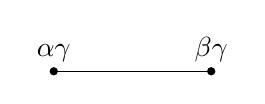
\begin{tikzpicture}[x=1cm,y=1cm]
\draw (0,0)--(2,0);
\fill (0,0) circle (1.5pt);
\fill (2,0) circle (1.5pt);
\node[above] at (0,0) {$\alpha\gamma$};
\node[above] at (2,0) {$\beta\gamma$};
\end{tikzpicture}
\end{adjustbox}
\end{center}
2 — || —
\begin{center}
\begin{adjustbox}{max width=\linewidth}
\begin{tikzpicture}[x=1cm,y=1cm]
\draw[very thick] (0,0)--(.45,1)--(1.15,0)--cycle;
\fill (0,0) circle (1.5pt);
\fill (.45,1) circle (1.5pt);
\fill (1.15,0) circle (1.5pt);
\node[above right] at (.45,1) {$\alpha\beta$};
\node[below left] at (0,0) {$\alpha\gamma$};
\node[below right] at (1.15,0) {$\beta\gamma$};
\draw (3.3,0)--(3.9,1)--(5,0)--cycle;
\node[above right] at (3.9,1) {$\alpha\delta$};
\node[below left] at (3.3,0) {$\gamma\delta$};
\node[below right] at (5,0) {$\beta\delta$};
\node[right] at (5.8,.6) {\underline{их — 2 типа.}};
\end{tikzpicture}
\end{adjustbox}
\end{center}

$n$-мерный гиперсимплекс — многогр., у к-го вершины — 0-мерные
гиперсимплексы, рёбра — 1-мерные гиперсимплексы и т.д.

% Triangle source [170,2540,500,2800), inspected at 4x. The lower-right outer vertex has no confidently visible numeral.
\begin{center}
\begin{adjustbox}{max width=\linewidth}
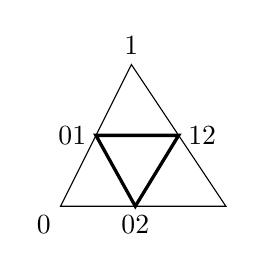
\begin{tikzpicture}[x=1cm,y=1cm]
\draw (0,0)--(.9,1.8)--(2.1,0)--cycle;
\draw[very thick] (.45,.9)--(1.5,.9)--(.95,0)--cycle;
\node[below left] at (0,0) {$0$};
\node[above] at (.9,1.8) {$1$};
\node[left] at (.45,.9) {$01$};
\node[right] at (1.5,.9) {$12$};
\node[below] at (.95,0) {$02$};
\end{tikzpicture}
\end{adjustbox}
\end{center}
\SourceFigure{GELFAND-P000695}{tetrahedral-hypersimplex}{Справа от треугольника: пространственный многогранный рисунок с внешними подписями $0$ слева внизу, $1$ внизу, $2$ справа и $3$ вверху. Жирные внутренние рёбра соединяют отмеченные вершины с подписями $03$, $23$, $13$, $01$, $12$; ещё одна подпись и часть пересечений во внутренней области не читаются уверенно.}
более сложные страты

% The following text is a right-hand side note, separated from the two drawings by two vertical strokes.
[Справа от рисунков, за двумя вертикальными чертами:]
В октаэдре встреч. 3-уг. 2-х типов.
\underline{Вып. оболочка мн-ва центров граней симплекса.}
В вершинах — индексы, соотв. индексам вершин соотв. грани.
Можно и дописывать всюду один и тот же индекс.

\underline{$Z(e_1,e_2)$} — соотв.
\begin{center}
\begin{adjustbox}{max width=\linewidth}
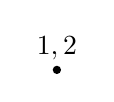
\begin{tikzpicture}
\fill (0,0) circle (1.5pt);
\node[above] at (0,0) {$1,2$};
\end{tikzpicture}
\end{adjustbox}
\end{center}
$Z^1(e_1,e_2,e_3)$. соотв.
\begin{center}
\begin{adjustbox}{max width=\linewidth}
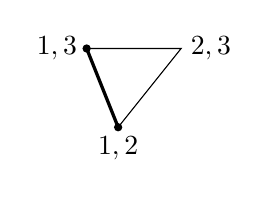
\begin{tikzpicture}[x=1cm,y=1cm]
\draw (0,1)--(1.2,1)--(.4,0)--cycle;
\draw[very thick] (0,1)--(.4,0);
\fill (0,1) circle (1.5pt);
\fill (.4,0) circle (1.5pt);
\node[left] at (0,1) {$1,3$};
\node[right] at (1.2,1) {$2,3$};
\node[below] at (.4,0) {$1,2$};
\end{tikzpicture}
\end{adjustbox}
\end{center}
\underline{Задача}: построить цепи по каждому гиперсимплексу с нужными
свойствами.

\SourcePage{GELFAND-P000696}{unlabelled}
% Review boxes are original-source pixels [x0,y0,x1,y1), origin upper left.
% Enlargement factors describe display scaling, not additional source detail.
% Reviewed whole-page: [0,0,2415,3471) at 1x.
% Reviewed top: [130,10,1720,405) at 3x.
% Reviewed diagrams: [110,385,2130,765) at 3x.
% Reviewed fan: [1780,60,2060,305) at 6x.
% Reviewed left-coefficient: [660,435,1060,590) at 5x.
% Reviewed cancelled-phrase: [135,650,460,735) at 6x.
% Reviewed lower-strokes: [630,600,1390,730) at 5x.
% Original inspected in full at 2415 x 3471; the page below the writing and diagrams is blank.
Цепь в пр-ве наборов векторов на плоскости.
Точке \underline{\underline{$12$}} — в пр-ве пар векторов $e_1=e_2=0$
Отрезку
\begin{center}
\begin{adjustbox}{max width=\linewidth}
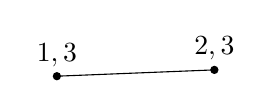
\begin{tikzpicture}[x=1cm,y=1cm]
\draw (0,0)--(2,.08);
\fill (0,0) circle (1.5pt);
\fill (2,.08) circle (1.5pt);
\node[above] at (0,0) {$1,3$};
\node[above] at (2,.08) {$2,3$};
\end{tikzpicture}
\end{adjustbox}
\end{center}
отвечает $(e_1=\lambda e_2,\ e_3=0)$.
$(3\text{ — лишнее!})$

% Source upper-right fan [1780,60,2060,305), inspected at 6x.
\begin{center}
\begin{adjustbox}{max width=\linewidth}
\begin{tikzpicture}[x=1cm,y=1cm]
\draw[->] (0,0)--(1.2,.15) node[right] {$e_1$};
\draw[->] (0,0)--(.7,1) node[right] {$e_2$};
\draw[->] (0,0)--(-.05,1.25) node[above left] {$e_3$};
\draw[->] (0,0)--(-1.35,.45) node[below left] {$e_4$};
\draw[->] (0,0)--(-.65,-1.1) node[below right] {$e_5$};
\end{tikzpicture}
\end{adjustbox}
\end{center}

% Both source triangles inspected in [110,385,2130,765) at 3x; coefficient verified separately at 5x.
\begin{center}
\begin{adjustbox}{max width=\linewidth}
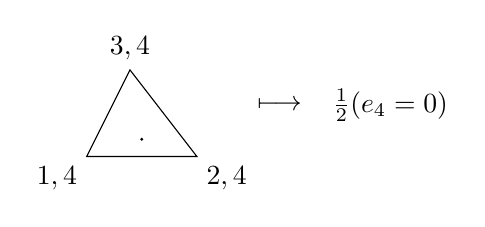
\begin{tikzpicture}[x=1cm,y=1cm]
\draw (0,0)--(.55,1.1)--(1.4,0)--cycle;
\fill (.7,.22) circle (.6pt);
\node[above] at (.55,1.1) {$3,4$};
\node[below left] at (0,0) {$1,4$};
\node[below right] at (1.4,0) {$2,4$};
\node at (2.45,.65) {$\longmapsto$};
\node[right] at (3,.65) {$\frac12(e_4=0)$};
\end{tikzpicture}
\end{adjustbox}
\end{center}

\begin{center}
\begin{adjustbox}{max width=\linewidth}
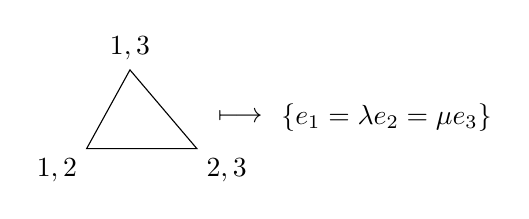
\begin{tikzpicture}[x=1cm,y=1cm]
\draw (0,0)--(.55,1)--(1.4,0)--cycle;
\node[above] at (.55,1) {$1,3$};
\node[below left] at (0,0) {$1,2$};
\node[below right] at (1.4,0) {$2,3$};
\node at (1.95,.4) {$\longmapsto$};
\node[right] at (2.35,.4) {$\{e_1=\lambda e_2=\mu e_3\}$};
\end{tikzpicture}
\end{adjustbox}
\end{center}

\Incomplete{GELFAND-P000696}{cancelled-phrase}{Под левым треугольником находится зачёркнутая фраза; текст не удалось прочитать.}
\SourceFigure{GELFAND-P000696}{lower-strokes}{Под треугольниками: два длинных почти горизонтальных штриха, каждый с утолщённым или заострённым левым концом; между штрихами отдельная точка. Первый штрих слегка поднимается вправо. Подписей непосредственно у штрихов нет.}

\SourcePage{GELFAND-P000697}{unlabelled}
% Review boxes are original-source pixels [x0,y0,x1,y1), origin upper left.
% Enlargement factors describe display scaling, not additional source detail.
% Reviewed whole-page: [0,0,2415,3471) at 1x.
% Reviewed top: [110,0,2320,610) at 3x.
% Reviewed middle: [120,610,2360,1280) at 3x.
% Reviewed forms: [180,1300,2290,2230) at 3x.
% Reviewed bottom: [100,2230,2260,3430) at 3x.
% Reviewed integral-cancellation: [665,440,750,535) at 10x.
% Reviewed integral-context: [355,425,920,550) at 5x.
% Reviewed wf-relation: [715,1090,805,1170) at 10x.
% Reviewed wf-context: [380,1045,1050,1215) at 5x.
% Reviewed direction: [650,1180,1020,1300) at 4x.
% Reviewed form-operator: [420,1430,560,1515) at 10x.
% Reviewed operator-repeat: [440,1660,565,1750) at 10x.
% Reviewed cycle-dimension: [1330,2330,1970,2420) at 3x.
% Reviewed coefficients: [410,2460,1100,2740) at 4x.
% Reviewed last-word: [430,3280,620,3375) at 6x.
% Original inspected in full at 2415 x 3471. Heading is visible in this frame; no catalogue heading has been supplied.
\underline{21/III — 77 г.}\qquad \underline{\underline{Сем. Гельфанда.}}

\underline{М. И. Граев.}
Рассм. $\mathbb{C}^3$ и там ф-ю $f(x)=f(x_1,x_2,x_3)$.
Рассм. прямую
\begin{equation*}
\begin{cases}
x_1=\alpha_1x_3+\beta_1\\
x_2=\alpha_2x_3+\beta_2
\end{cases}
\end{equation*}
\begin{equation*}
\int f(\alpha_1x_3+\beta_1\,\text{[зачёркнуто]},\,
\alpha_2x_3+\beta_2,x_3)\,dx_3\,d\bar{x}_3
=\varphi(\alpha_1,\alpha_2;\beta_1,\beta_2)
\end{equation*}
\Unclear{GELFAND-P000697}{integral-cancel}{Непосредственно после $\beta_1$ в первом аргументе $f$: зачёркнутый неразборчивый знак.}
Как по $\varphi$ восстановить $f$? Задача переопред. и тривиальная.

% Source quadrilateral and interior point, upper-left [235,650,440,825), inspected in 3x middle crop.
\begin{center}
\begin{adjustbox}{max width=\linewidth}
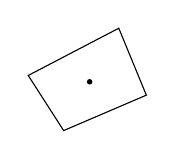
\begin{tikzpicture}[x=1cm,y=1cm]
\draw (0,.6)--(1.15,1.2)--(1.5,.35)--(.45,-.1)--cycle;
\fill (.78,.52) circle (1pt);
\end{tikzpicture}
\end{adjustbox}
\end{center}
Провед. плоскость. Возникнет классич. зад. Радона. Её реш. хорошо известно.
Решение. Пишется $(1,1)$-форма на мн-ве прямых, кот. в плоск.
Её интеграл даёт ответ.
В вещ. случае ур-е
\begin{equation*}
\frac{\partial^2\varphi}{\partial\alpha_1\partial\beta_2}
=\frac{\partial^2\varphi}{\partial\alpha_2\partial\beta_1}.
\end{equation*}
Можно док., что оно достаточно.

\underline{Идея}
$\underline{WF(u)}\ni(x_0,\xi_0)$, если интеграл по системе паралл.
плоскостей с напр. $\xi_0$ имеет особенность.

Построим дифф. форму
\Unclear{GELFAND-P000697}{form-operator}{Знак оператора перед $\varphi$ в следующих формулах: $\mathcal{H}$ или Ж; ниже воспроизведён кандидат $\mathcal{H}$.}
\begin{align*}
\mathcal{H}\varphi
&=\sum_{i,j=1}^{2}\frac{\partial^2\varphi}{\partial\beta_i\partial\bar{\beta}_j}\,
 d\alpha_i\wedge d\bar{\alpha}_j \qquad (\mathbb{C}^3)\\
\mathcal{H}\varphi
&=\frac{\partial\varphi}{\partial\beta_1}\,d\alpha_1
 +\frac{\partial\varphi}{\partial\beta_2}\,d\alpha_2 \qquad (\mathbb{R}^3)
\end{align*}
Пусть есть точка $(x_1^0,x_2^0,x_3^0)$. Подставляем $\beta_i=x_i^0-\alpha_i x_3^0$.
Получ. огранич. формы на прямые, прох. через эту точку.
Это обозначим $\mathcal{H}_{x^0}\varphi$.
\Unclear{GELFAND-P000697}{form-operator}{В $\mathcal{H}_{x^0}\varphi$ повторён тот же неуверенно читаемый знак оператора.}

\underline{Теорема}.
$\varphi$ \underline{представима через $f$} $\Leftrightarrow$
$d(\mathcal{H}_{x^0}\varphi)=0$, $\forall x_0$.
\Unclear{GELFAND-P000697}{form-operator}{В $d(\mathcal{H}_{x^0}\varphi)$ повторён тот же неуверенно читаемый знак оператора.}

\underline{Формула обращения} в $\mathbb{C}^3$ (в $\mathbb{R}^3$ она уже нелокальна).
Выделим в прямых, прох. через $x_0$, \Unclear{GELFAND-P000697}{cycle-dimension}{1-мерный} цикл $\gamma$ и тогда
\begin{equation*}
\underline{\int_\gamma\mathcal{H}_{x^0}\varphi
=c_\gamma f(x^0)}
\end{equation*}
\Unclear{GELFAND-P000697}{form-operator}{Под интегралом повторён тот же неуверенно читаемый знак оператора $\mathcal{H}$.}
В вещ. случае $C_\gamma=0$.
\Unclear{GELFAND-P000697}{coefficient-case}{Буква коэффициента в $C_\gamma=0$: $C_\gamma$ или $c_\gamma$.}

Комплекс $K$ — 3-мерное мн-зие прямых
Когда, зная $\mathcal{H}\varphi$ на $K$, можно восстановить $\varphi$?
\Unclear{GELFAND-P000697}{form-operator}{В вопросе о комплексе $K$ повторён тот же неуверенно читаемый знак $\mathcal{H}$ перед $\varphi$.}
Все комплексы $K$, облад. этим св-вом, таковы:

а) все прямые, касающиеся поверхности

б) — || —, пересекающие кривую

\underline{Линейный комплекс} — компл. прямых в $\mathbb{C}P^3$ $(\mathbb{R}P^3)$.
все прямые его, прох. через данную точку — плоскость.

\SourcePage{GELFAND-P000698}{unlabelled}
% Review boxes are original-source pixels [x0,y0,x1,y1), origin upper left.
% Enlargement factors describe display scaling, not additional source detail.
% Reviewed plucker-word: [230,240,575,350) at 10x.
% Original: images/GELFAND-P000698.png; 2415 x 3471 pixels.
% Review coordinates use [x0,y0,x1,y1), origin at upper left; no new source pixels were created.
% Whole original inspected at native resolution. Content occupies approximately y=35..1190; lower remainder blank.
% Enlarged regions: matrix [170,35,840,230) x3; plucker [220,240,2200,350) x3;
% linear-equation [210,342,1280,460) x3; complex-point [190,475,1750,570) x3;
% parenthetical [1735,475,2330,635) x3; complex-line [190,590,2315,745) x3;
% example [905,745,1260,960) x5; isomorphic [70,925,925,1030) x3;
% correction [95,940,295,1020) x10; references [170,1020,1660,1185) x3;
% reference-number [695,1085,900,1168) x6; reference-chapters [445,1010,800,1105) x5;
% last-name [1410,1085,1660,1190) x5.
\begin{equation*}
\begin{array}{c}x\\y\end{array}
\quad
\begin{Vmatrix}
x_1 & x_2 & x_3 & x_4\\
y_1 & y_2 & y_3 & y_4
\end{Vmatrix}
\end{equation*}

Плюккеровы координаты $p_{ij}=x_i y_j-x_j y_i$ — координаты плоскости.

Лин. комплекс: $\sum c_{ij}p_{ij}=0$.

\underline{Лин. комплекс.} [Волнистое подчёркивание.]
с $\forall$ точкой пр-ва связана плоскость
(в ней лежат все прох. через неё пр.)

с $\forall$ прямой связана прямая, пересек. все прямые, прох. через исходную.

Преобр. Лежандра есть.

\underline{Пример комплекса.} [Волнистое подчёркивание.]
\begin{align*}
x_1&=\alpha x_3+\beta\\
x_2&=\gamma x_3+\alpha
\end{align*}

\Unclear{GELFAND-P000698}{isomorphic-correction}{Любой [последняя буква исправлена; прежние штрихи неразборчивы]}
другой ему изоморфен.

\underline{Лит-ра}: 1 и 2 главы 5-го вып. обобщ. ф-й.

Ф. А., т. 1, $N=1$, раб. Гельфанд, Граев, Шапиро.
\SourcePage{GELFAND-P000699}{unlabelled}
% Independent review coordinates below use original pixels, top-left origin, [x0,y0,x1,y1).
% Review 699-ref: bbox=[215, 1880, 2260, 2080]; enlargement=2x; original source inspected too.
% Review 699-groups: bbox=[780, 3220, 2200, 3410]; enlargement=4x; original source inspected too.
% Original frame: 2415 x 3471 pixels. Blank upper field inspected; no page or leaf label read.
% Review: date and seminar heading bbox=(210,1130,1170,1240), inspected original and 3x crop.
\underline{28/III-77г.}\qquad \underline{Сем. Гельфанда.}

\underline{И.М. Гельфанд.}\qquad
\underline{Задача} (из раб. Гриффитса
\Unclear{GELFAND-P000699}{griffiths-cancellation}{[зачёркнутый знак неразборчив]}:
Вариации на тему теоремы Абеля.)

В окружности --- эллипс.

\SourceFigure{GELFAND-P000699}{poncelet-figure}{Окружность, внутри неё горизонтально вытянутый овал и наложенные друг на друга прямолинейные стороны вписанных фигур. Видны две близкие верхние вершины, две близкие вершины слева внизу и два окончания справа; пересечения и соединения сторон местами утолщены и не вполне различимы. Подписей нет.}

Многоугольник; впис. в 1 кривую 2-го пор. и опис. вокруг другой.
\underline{Когда это так?} (Когда можно вписать так?)

\underline{Теор. Понселе}: если из одной точки замыкается, то из $\forall$ другой
замкн. через столько же шагов

\underline{Якоби}: некое соотнош. в эллиптич. интегралах

Из теор. Понселе $\Rightarrow$ $\exists$ инвар. мера и изом. повороту окружности.

Посл. номер
\Unclear{GELFAND-P000699}{journal-title}{Compositia Math.}
--- самое простое док-во теор. \underline{Дворецкого}.

(\underline{Фигель})
% Review: surname bbox=(1650,1900,2300,2030), name bbox=(455,1985,735,2140), inspected 5x and independently rechecked; retained Дворецкого and Фигель.

\underline{А.М. Вершик.}\qquad
\underline{Теория вероятностей и симм. группа}

$S_n$ --- гр. подстановок мн-ва из $n$ элем.

$S_\infty$ --- гр. финитных вз.-однозн. подстан. натур. ряда, затраг. лишь
\Unclear{GELFAND-P000699}{finite-cancellation}{[зачёркнутые буквы неразборчивы]}
конечное число элементов

\underline{Асимпт. задачи, связ. с $S_n$} --- асимпт. меры Планшереля.

\underline{Таблица Юнга.}\qquad
Набор строк, начинающ. у вертик. линии и убыв. длины

% Review: Young diagram bbox=(225,2700,745,3150), inspected 5x. Five rows of lengths 5,4,3,1,1; upper line continues right; left line continues downward with arrow.
\begin{center}
\begin{adjustbox}{max width=\linewidth}
\begin{tikzpicture}[x=0.42cm,y=0.42cm]
\draw (0,0) -- (7.4,0);
\draw[->] (0,0) -- (0,-6.8);
\draw (0,-1) -- (5,-1) -- (5,0);
\draw (0,-2) -- (4,-2) -- (4,0);
\draw (0,-3) -- (3,-3) -- (3,0);
\draw (0,-4) -- (1,-4);
\draw (0,-5) -- (1,-5) -- (1,0);
\draw (2,0) -- (2,-3);
\node at (2.5,-4.2) {$\Lambda$};
\end{tikzpicture}
\end{adjustbox}
\end{center}

(см. конец кн. Ван-дер Вардена\newline
Кэртис, Райнер,\newline
Кириллов

Пусть $n$ клеток;

Подгруппа
\begin{equation*}
\begin{array}{ccc}
G_1,&G_2\subset S_n&\\
\vert&\vert&\\
\text{сохр. разб.}&\text{сохр. разб.}&\\
\text{на строки}&\text{на столбцы}&\\
S_n^{<}&S_n^{\Lambda}&\text{--- перест. элем внутри столбца.}
\end{array}
\end{equation*}
\Unclear{GELFAND-P000699}{row-subgroup-symbol}{$S_n^{<}$: верхний знак, похожий на повёрнутую $\Lambda$}


\Unclear{GELFAND-P000699}{bottom-cancellation}{[Зачёркнуто: Все предс.]}

\SourcePage{GELFAND-P000700}{unlabelled}
% Independent review coordinates below use original pixels, top-left origin, [x0,y0,x1,y1).
% Review 700-bottom: bbox=[70, 2870, 2395, 3390]; enlargement=2x; original source inspected too.
% Review 700-adjective: bbox=[370, 20, 750, 145]; enlargement=6x; original source inspected too.
% Review 700-bottom-spectrum: bbox=[1250, 2970, 2330, 3115]; enlargement=4x; original source inspected too.
% Review 700-bottom-cancel: bbox=[150, 3090, 2405, 3170]; enlargement=4x; original source inspected too.
% Review 700-regular-operator: bbox=[955, 2410, 1250, 2550]; enlargement=6x; original source inspected too.
% Original frame: 2415 x 3471 pixels. Entire page and outer margins inspected; no page or leaf label read.
Рассм. \Unclear{GELFAND-P000700}{top-adjective}{единична} предст. $S_n^{<}$
и \underline{1-мерное} у $S_n^{\Lambda}$
\Unclear{GELFAND-P000700}{top-subgroup-symbol}{$S_n^{<}$: верхний знак, похожий на повёрнутую $\Lambda$}

(чётным --- единичн. 1\newline
нечётным --- $(-1)$) $\longleftarrow$ сигнатурное предст.

Индуцируем с каждого такого предст. предст. $S_n$

Они приводимы, но у них есть \underline{единств. общее неприводимое} (теорема!)
--- оно и сопоставляется.

\underline{1955.} ф-ла крюков (Робинсон и др.)

hook

Крюк --- общее число клеток правее и ниже данной ---

% Review: hook sketch bbox=(245,565,610,840), inspected 3x. Stepped outer contour, a bent inner line with endpoints, and a leftward pointing annotation arrow.
\begin{center}
\begin{adjustbox}{max width=\linewidth}
\begin{tikzpicture}[x=0.65cm,y=0.65cm]
\draw (0,0) -- (0,1.9) -- (1.45,1.9);
\fill (0,0) circle (0.035);
\fill (0,1.9) circle (0.035);
\fill (1.45,1.9) circle (0.035);
\draw (-0.2,-0.3) -- (0.45,-0.18) -- (0.45,0.9) -- (0.98,0.9) -- (0.98,1.48) -- (1.7,1.52) -- (1.62,2.26);
\draw[<-] (1.08,0.9) -- (1.95,0.9);
\node[anchor=west] at (2.02,0.9) {здесь 6 клеток в крюке};
\end{tikzpicture}
\end{adjustbox}
\end{center}

\begin{equation*}
\frac{n!}{\prod h_{ij}}=\dim\Lambda
\end{equation*}
$h_{ij}$ ---
\Unclear{GELFAND-P000700}{hook-definition-cancellations}{[два зачёркнутых слова неразборчивы]}
(--- число элем. в крюке

\Unclear{GELFAND-P000700}{graph-heading-mark}{[густо заштрихованный знак]}
\underline{Граф Юнга.} Вершины --- таблицы Юнга. В $n$-м столбце ---
табл. из $n$ клеток.

Рёбра --- когда можно получить присоединением одной клетки.

% Review: Young graph bbox=(265,1000,1080,1510), inspected 3x; top-right overdraw inspected 10x.
% Only visible graph edges are reproduced. No edge from the middle three-cell shape to the four-cell hook below was added.
\begin{center}
\begin{adjustbox}{max width=\linewidth}
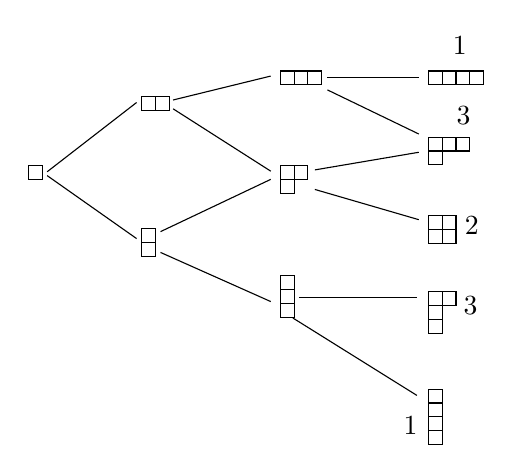
\begin{tikzpicture}[x=0.8cm,y=0.8cm]
\draw (0.00,0.00) rectangle (0.22,-0.22);
\draw (1.80,1.10) rectangle (2.02,0.88);
\draw (2.02,1.10) rectangle (2.24,0.88);
\draw (1.80,-1.00) rectangle (2.02,-1.22);
\draw (1.80,-1.22) rectangle (2.02,-1.44);
\draw (4.00,1.50) rectangle (4.22,1.28);
\draw (4.22,1.50) rectangle (4.44,1.28);
\draw (4.44,1.50) rectangle (4.66,1.28);
\draw (4.00,0.00) rectangle (4.22,-0.22);
\draw (4.22,0.00) rectangle (4.44,-0.22);
\draw (4.00,-0.22) rectangle (4.22,-0.44);
\draw (4.00,-1.75) rectangle (4.22,-1.97);
\draw (4.00,-1.97) rectangle (4.22,-2.19);
\draw (4.00,-2.19) rectangle (4.22,-2.41);
\draw (6.35,1.50) rectangle (6.57,1.28);
\draw (6.57,1.50) rectangle (6.79,1.28);
\draw (6.79,1.50) rectangle (7.01,1.28);
\draw (7.01,1.50) rectangle (7.23,1.28);
\draw (6.35,0.45) rectangle (6.57,0.23);
\draw (6.57,0.45) rectangle (6.79,0.23);
\draw (6.79,0.45) rectangle (7.01,0.23);
\draw (6.35,0.23) rectangle (6.57,0.01);
\draw (6.35,-0.80) rectangle (6.57,-1.02);
\draw (6.57,-0.80) rectangle (6.79,-1.02);
\draw (6.35,-1.02) rectangle (6.57,-1.24);
\draw (6.57,-1.02) rectangle (6.79,-1.24);
\draw (6.35,-2.00) rectangle (6.57,-2.22);
\draw (6.57,-2.00) rectangle (6.79,-2.22);
\draw (6.35,-2.22) rectangle (6.57,-2.44);
\draw (6.35,-2.44) rectangle (6.57,-2.66);
\draw (6.35,-3.55) rectangle (6.57,-3.77);
\draw (6.35,-3.77) rectangle (6.57,-3.99);
\draw (6.35,-3.99) rectangle (6.57,-4.21);
\draw (6.35,-4.21) rectangle (6.57,-4.43);
\draw (0.3,-0.1) -- (1.72,1.0);
\draw (0.3,-0.16) -- (1.72,-1.16);
\draw (2.3,1.04) -- (3.85,1.42);
\draw (2.3,0.9) -- (3.85,-0.09);
\draw (2.1,-1.05) -- (3.85,-0.22);
\draw (2.1,-1.38) -- (3.85,-2.16);
\draw (4.75,1.4) -- (6.2,1.4);
\draw (4.75,1.2) -- (6.2,0.5);
\draw (4.55,-0.07) -- (6.2,0.21);
\draw (4.55,-0.38) -- (6.2,-0.86);
\draw (4.3,-2.1) -- (6.17,-2.1);
\draw (4.2,-2.42) -- (6.17,-3.65);
\node at (6.85,1.9) {$1$};
\node at (6.91,0.79) {$3$};
\node at (7.04,-0.96) {$2$};
\node at (7.02,-2.22) {$3$};
\node at (6.07,-4.13) {$1$};
\end{tikzpicture}
\end{adjustbox}
\end{center}
\SourceFigure{GELFAND-P000700}{young-graph-top-overdraw}{Верхняя правая вершина графа: горизонтальная строка примерно из четырёх клеток, над ней 1. Левые и средние внутренние штрихи многократно обведены и частично слились. В рисунке выше передан различимый прямоугольный контур; подробности этих наложенных штрихов сохраняются в источнике.}

\underline{Теор. ветвления.}\qquad
$S_n$; $\pi$ --- \underline{неприв. предст.} $S_n$

$S_{n-1}\subset S_n$

В $\pi|_{S_{n-1}}$ \underline{любое неприв. предст. встреч. с крат. 1}.

\Unclear{GELFAND-P000700}{branching-cancellation}{[зачёркнутое слово неразборчиво]}
\textit{[Над зачёркнутым словом вписано и обведено: Диагр.]}
на $n$-м шагу разлагается именно на предшествующие.

--- Одномерных подпр-в --- столько, сколько путей в графе, довод. до 1.

--- Отсюда счёт --- комбинат. задача, к-рая не решена (только через ф-лу Фробениуса и т. д.)

Базис Гельфанд --- Цетлина
% Review: heading bbox=(85,1990,915,2070), inspected 5x. Source visibly has Гельфанд without a final а.

\underline{Вопрос}: $S_m\subset S_n$.
\Unclear{GELFAND-P000700}{question-cancellation}{[зачёркнутое короткое слово неразборчиво]}
сколько путей доходит до фикс. табл. Юнга?

Длина 1-й строки
\begin{equation*}
\ell_1(\Lambda)=\max\{m:\ \pi|_{S_m}\supset\mathrm{id}\}
\end{equation*}

Регулярное предст.
\Unclear{GELFAND-P000700}{regular-superscripts}{$C(S^n)$ --- ф-и на $S^n$}
% Review: bbox=(890,2325,1645,2435), inspected 5x. Both n's are superscripts in the source; not changed to subscripts.
\begin{equation*}
(U_gf)(h)=f(g^{-1}h)
% Review: operator bbox=(920,2430,1510,2550), inspected 8x. U has a rounded lower join and two upper stems; retained U_g.
\end{equation*}

\underline{Мера Планшереля на табл. Юнга}

Изв., что
\begin{equation*}
n!=\sum_{\Lambda}(\dim\Lambda)^2
\end{equation*}
--- разм. рег. предст.
% Review: n! annotation bbox=(225,2780,670,2935), inspected 5x; phrase retained below the display.

мера Планшереля
\begin{equation*}
\mu(\Lambda)=\frac{(\dim\Lambda)^2}{n!}
\end{equation*}

\underline{Зад. Гельфанда.}

Дать интерпрет. меры Планшереля беск.-мерного предст.
($\overset{\text{на}}{\text{непр.}}$ спектре)
% Review: bbox=(95,2950,2415,3095), inspected 5x and independently rechecked. на is inserted above the beginning of the parenthetical phrase.

\textit{[Вписано над зачёркнутой строкой:]} Рассм. меру на пр-ве путей в таблицах

\textit{[Зачёркнуто:]} Пусть на табл. из $n$ клеток зад. мера

\textit{[Зачёркнуто:]} Пусть есть мера на таблицах из $n$
\Unclear{GELFAND-P000700}{bottom-right-cancellation}{клет...}

Пусть добавл. клетки. Рассм. \underline{усл. вероятность появл. клетки}
при известной истории

\SourcePage{GELFAND-P000701}{unlabelled}
% Independent review coordinates below use original pixels, top-left origin, [x0,y0,x1,y1).
% Review 701-clt: bbox=[125, 1800, 2355, 2150]; enlargement=2x; original source inspected too.
% Review 701-abbrev: bbox=[1040, 510, 1810, 710]; enlargement=4x; original source inspected too.
% Review 701-attribution: bbox=[170, 2800, 1140, 3000]; enlargement=4x; original source inspected too.
% Review 701-length: bbox=[205, 2600, 1785, 2740]; enlargement=4x; original source inspected too.
% Review 701-omega-side: bbox=[1745, 990, 2360, 1190]; enlargement=5x; original source inspected too.
% Original frame 2415 x 3471. No confidently visible page/leaf label.
% Reviewed top drawing bbox [245,130,1030,610], including 3x crop.
\underline{Теорема}

\begin{adjustbox}{max width=\linewidth}
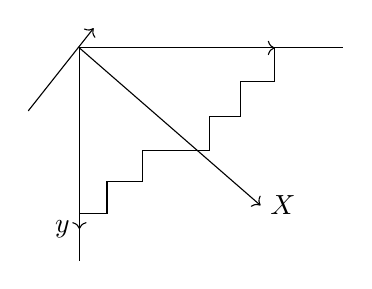
\begin{tikzpicture}[x=1cm,y=1cm]
\draw[->] (-0.65,-0.8) -- (0.18,0.25);
\draw[->] (0,0) -- (2.48,0);
\draw (2.48,0) -- (3.35,0);
\draw[->] (0,0) -- (0,-2.3);
\draw (0,-2.3) -- (0,-2.7);
\node[left] at (0,-2.3) {$y$};
\draw[->] (0,0) -- (2.3,-2);
\node[right] at (2.3,-2) {$X$};
\draw (0,-2.1) -- (0.35,-2.1) -- (0.35,-1.7) -- (0.8,-1.7) -- (0.8,-1.3) -- (1.65,-1.3) -- (1.65,-0.87) -- (2.05,-0.87) -- (2.05,-0.43) -- (2.48,-0.43) -- (2.48,0) -- (3.35,0);
\end{tikzpicture}
\end{adjustbox}

Рассм. сист. коорд.
\begin{equation*}
\begin{array}{||l}
X=\frac{x+y}{2};\\
Y=\frac{x-y}{2};
\end{array}
\end{equation*}

Рассм. график ф-и $|X|$, \Unclear{GELFAND-P000701}{young-abbreviation}{укр.?}
\Unclear{GELFAND-P000701}{young-correction}{зачёркнуто: диаграммой?; сверху вписано: таблицей}
Юнга

% Reviewed bbox [240,680,923,790], 4x: visible singular «Таблица».
Таблица отожд. с ф-ей $Y=\widetilde\Lambda(X)$
\begin{equation*}
\mu_n\left\{\widetilde\Lambda:\ \sup\left|\frac{1}{\sqrt n}\widetilde\Lambda(\sqrt n\,X)-\Omega(X)\right|<\varepsilon\right\}\longrightarrow1,\qquad\forall\varepsilon>0
\end{equation*}
сожмем в $\sqrt n$ раз. Тогда все в окр. графика ф-и
\begin{equation*}
\Omega(X)=\frac{2}{\pi}\left(X\arcsin X+\sqrt{1-X^2}\right)
\qquad
\left(\Omega'(X)=\frac{2}{\pi}\arcsin X\right)
\end{equation*}

Это сход. по мере, \Unclear{GELFAND-P000701}{convergence-cancellation}{зачёркнут короткий знак или фрагмент}
Есть теор. о сход. почти всюду. (для послед. таблиц)

Диаграмма --- беск. путь. Для почти всех диагр. сходится.
% Reviewed curve bbox [240,1470,610,1730]; unlabelled horizontal/vertical strokes and curved arrow retained.
\begin{adjustbox}{max width=\linewidth}
\begin{tikzpicture}[x=1cm,y=1cm]
\draw (0,-1.55) -- (0,0) -- (2.3,0);
\draw[->] (0,-1.5) .. controls (0,-0.5) and (0.75,-0.05) .. (1.8,0);
\end{tikzpicture}
\end{adjustbox}

\underline{Следствие:}
\begin{equation*}
\mu_n\left\{\Lambda:\ \left|\frac{\ell_1(\Lambda)}{2\sqrt n}-1\right|<\varepsilon\right\}
\end{equation*}
% Reviewed bbox [720,1410,2070,1790], 2x: no limit arrow supplied after the displayed set; retained as written.
(с вер., близкой к 1, есть инвар. вектор)

(решение зад. Улама)

Это закон больших чисел. Уклонения дают белый шум.

Для функционала $\int f(X)\Lambda(X)\,dX$ есть центр. пред. теор.
% Reviewed CLT scale factors bbox [180,1970,1710,2170], 3x; numerator radical rechecked 10x at [415,1980,565,2145].
% Both visible radical indices are 4; the source's fourth-root scales are retained without correction.
\begin{equation*}
\mu_n\left\{\Lambda:\ \frac{1}{\sqrt[4]{n}}\int f(X)\Lambda(\sqrt[4]{n}\,X)\,dX-\int f(X)\Omega(X)\,dX<\ell\right\}\longrightarrow\varphi_f(\ell,\varepsilon)
\end{equation*}
\Unclear{GELFAND-P000701}{clt-limit}{Правая часть предположительно $\varphi_f(\ell,\varepsilon)$; перед $\ell$ густая правка.}

марковость и стационарность проверяются.

\Unclear{GELFAND-P000701}{cancelled-tuple}{зачёркнутая запись перед $(x_1,\ldots,x_n)$; видны скобка, $x_1$ и конечный индекс $n$}
\begin{equation*}
(x_1,\ldots,x_n),\qquad
\overset{\substack{\underline{\text{равном. распред.}}\\\swarrow}}{0\le x_i\le1};\quad i=1,\ldots,n
\end{equation*}

% Reviewed bbox [185,2405,2180,2600], 2x and [500,2390,820,2515], 6x: «монот.».
Рассм. монот. возр. послед. (не обяз. подряд) Какова длина её?

\Unclear{GELFAND-P000701}{maximum-length}{$\max\{r:\ \exists\ i_1<\cdots<i_n,\ X_{i_1}\le X_{i_2}\le\cdots\le X_{i_n})$; первый знак читается как $r$, конечные индексы как $n$, закрывающая скобка круглая.}

растет как $\underline{\underline{2\sqrt n}}$ (по мере Лебега на ед. кубе)

\underline{1970}, Кнут, \Unclear{GELFAND-P000701}{attribution-name}{Рас. Јошп.?}

\underline{1961}, \Unclear{GELFAND-P000701}{attribution-cancellation}{перед фамилией зачёркнуты короткие буквенные штрихи} Shenstead

% Reviewed bbox [1185,2800,2110,2970], 3x: «Есть отобр. в диаграммы (вытеснение)».
\begin{equation*}
\begin{array}{||l}
\text{Есть отобр. в диаграммы}\\
\text{(вытеснение)}
\end{array}
\end{equation*}

\SourcePage{GELFAND-P000702}{unlabelled}
% Independent review coordinates below use original pixels, top-left origin, [x0,y0,x1,y1).
% Review 702-box: bbox=[1590, 1530, 2370, 1950]; enlargement=3x; original source inspected too.
% Review 702-bottom: bbox=[120, 3050, 2330, 3310]; enlargement=3x; original source inspected too.
% Review 702-relation: bbox=[1300, 2780, 2040, 2960]; enlargement=4x; original source inspected too.
% Review 702-bundle-question: bbox=[80, 3000, 1280, 3145]; enlargement=4x; original source inspected too.
% Review 702-fixed-curve: bbox=[1750, 2165, 2335, 2420]; enlargement=5x; original source inspected too.
% Original frame 2415 x 3471. Blank upper area inspected; content begins near y=1290. No visible page/leaf label.
% Visible heading independently read, not derived from catalogue association.
4/IV-77 г. \underline{Сем. Гельфанда.}

\underline{А. Тюрин.}

$FG_g$ --- группа с $2g$ образ. $a_1,\ldots,a_g,b_1,\ldots,b_g$ и соотн.
\begin{equation*}
\prod_i[a_i,b_i]=1;\qquad [a_i,b_i]=a_i b_i a_i^{-1}b_i^{-1}
\end{equation*}

$R_C$ --- мн-зие классов предст. в $GL(n,C)$

алгеб. мн-зие с особенностями.

% Right boxed note, bbox [1590,1530,2370,1950], reviewed at 3x; «Фактор. по подобию».
\begin{quote}
\textit{[В правом поле, в рамке:]}
наборов матр. $A_1,\ldots,A_{2g}$
\Unclear{GELFAND-P000702}{matrix-last-index}{Последний индекс в перечне матриц предположительно $2g$; густые мелкие штрихи.}

Разм. $2gn^2-n^2+1$

(1 т.к. $\det=1$ автом.,

Фактор. по подобию
\begin{equation*}
2gn^2-n^2+1-n^2+1=2(g-1)n^2+2
\end{equation*}
\end{quote}

\begin{equation*}
\pi_1(X)\longleftrightarrow FG_g
\end{equation*}
Предст. $\varrho\rightsquigarrow$ рассл. $E_{\varrho}$ на $X$

Аналит. \Unclear{GELFAND-P000702}{analytic-cancellation}{зачёркнутое сокращение: предст.?} эквив.
\begin{equation*}
\underset{\mathrm{def}}{\Longleftrightarrow}\qquad E_{\varrho_1}\cong E_{\varrho_2}
\end{equation*}
% Reviewed bbox [900,2080,1140,2205], enlarged: the annotation under the equivalence arrow reads def.

% Right-margin annotated quotient, bbox [1670,1920,2350,2130], reviewed at 3x.
\begin{equation*}
\underset{\pi_1}{U(X)}\times\underset{\varrho}{V^n}/\pi_1\longrightarrow X
\end{equation*}
\Unclear{GELFAND-P000702}{upper-quotient-vector}{В правой верхней записи множитель перед $/\pi_1$ предположительно $V^n$; первая буква сведена к почти вертикальному штриху.}

\underline{Пакет представлений}
\begin{equation*}
\underset{\substack{\uparrow\\\underline{\text{афф. пр-во разм.}}\ (n^2-1)(g-1)}}{H(X,E)}\subset R_C
\end{equation*}

% Final independent review: bbox [1750,2165,2335,2420], 5x, confirms Для.
Для фиксир. кривой $X$ и фиксир. рассл. $E$.

Пр-во предст. имеет размерность $2((g-1)n^2+1)$

% Final independent review: bbox [920,2560,1200,2670], 8x; final т compared with имеет at [625,2450,870,2575].
Предст. общего полож. будет неприв.

\begin{equation*}
E_{\varrho}=\underset{\substack{\uparrow\\\text{универс. накрывающая}}}{U(X)}\times V^n/\pi_1
\qquad x\in U(X)
\end{equation*}
% Reviewed quotient relation bbox [1300,2780,2040,2960], 4x/5x: vector xi and representation varrho distinguished visually.
\begin{equation*}
(x,\xi)\sim(xg,\varrho(g)\xi)
\end{equation*}

\Unclear{GELFAND-P000702}{bundle-question}{Расслоения связн.?} $\Rightarrow$ что можно сказать о предст.?

Любые два \Unclear{GELFAND-P000702}{irreducible-overwrite}{неприв.?} предст.
\Unclear{GELFAND-P000702}{equivalent-overwrite}{эквивал.; начало слова переписано поверх прежних штрихов}
относит. нек-рой рим. пов. (вх. в какой-то пакет).

Фиксируем $X\Rightarrow$
\begin{equation*}
R_C\overset{\substack{\text{аффинное расслоение}\\\swarrow}}{\longrightarrow}S_n(X)
\qquad\text{(модули рассл.)}
\end{equation*}

\SourcePage{GELFAND-P000703}{unlabelled}
% Independent review coordinates below use original pixels, top-left origin, [x0,y0,x1,y1).
% Review 703-middle: bbox=[160, 920, 2355, 1625]; enlargement=2x; original source inspected too.
% Review 703-top: bbox=[175, 25, 2280, 340]; enlargement=3x; original source inspected too.
% Review 703-verb: bbox=[1040, 1340, 2280, 1470]; enlargement=4x; original source inspected too.
% Review 703-jacobian: bbox=[205, 2150, 1970, 2460]; enlargement=3x; original source inspected too.
% Review 703-schwarzian-margin: bbox=[1270, 2780, 2340, 3250]; enlargement=3x; original source inspected too.
% Review 703-sections: bbox=[580, 640, 1050, 765]; enlargement=5x; original source inspected too.
% Review 703-other-reps: bbox=[1410, 1250, 2260, 1410]; enlargement=4x; original source inspected too.
% Review 703-properties: bbox=[150, 970, 740, 1090]; enlargement=5x; original source inspected too.
% Review 703-corollary: bbox=[145, 1920, 2130, 2190]; enlargement=3x; original source inspected too.
% Source frame 2415 x 3471 px. No legible documentary page/leaf label.
% Review top-heading [175,15,2240,305]: original and 3x/5x crops;
% «Типичная задача», «описание», H(X,L), and the superscript *2g checked.
\underline{Типичная задача}: рассм. пакеты представл., соотв. 1-мерн. рассл. $L$.

Как описание \Unclear{GELFAND-P000703}{top-description-word}{всё} мн-ва
$H(X,L)\subset\mathbb C^{*2g}$ — \underline{пр-во характеров}.

$L$ — 1-мерное расслоение.

% Review bundle-cocycles [265,285,2160,640], 3x;
% cohomology exponent at [1480,305,1810,405] checked at 7x: 1.
$L$: зад. ф-ями перехода
$\{\alpha_{ij}\}\in H^1(\{U_i\},\mathcal O_X^*)$.

$L$: получ. из
\Unclear{GELFAND-P000703}{bundle-cancelled-word}{[зачёркнуто: неразборчиво]}
предст. $\pi_1$
$\Leftrightarrow\{\alpha_{ij}\}\in H^1(X,\mathbb C^*)$
(можно взять $\alpha_{ij}=\mathrm{const}$).

Сечения: $f_i$ на
\Unclear{GELFAND-P000703}{sections-open-set}{$U_i$ / $U_j$ / $U_{ij}$}.
\begin{equation*}
f_i=\alpha_{ij}f_j.
\end{equation*}
% Review logarithmic-differential [120,640,2290,955], 3x.
\begin{equation*}
\alpha_{ij}=\mathrm{const}\quad\Rightarrow\quad
\frac{df_i}{f_i}=\omega\big|_{U_i}
\end{equation*}
— единый дифференциал (мероморфный).

% Final independent review: bbox [130,950,780,1110], 5x and [155,985,595,1090], 7x: Особенности.
\underline{Особенности} $\omega$: полюса $\leq1$-го порядка
\Unclear{GELFAND-P000703}{properties-cancelled-parenthesis}{[зачёркнуто: (дивизор?)]}.

Вычеты — целые числа.

Главн. части — дивизор
\begin{equation*}
[\omega]=\sum\operatorname{Res}_x\omega\cdot x
\end{equation*}
(нули и полюса ф-й $f_i$).

% Review representatives-note [1450,1260,2160,1402], 5x;
% two implication arrows are visible, one at each end of the line break.
2 другие представители $\Rightarrow$
\newline
$\Rightarrow$ экв. дивизор.

\underline{Фиксируем дивизор}.
\Unclear{GELFAND-P000703}{construction-cancelled-word}{[зачёркнуто: неразборчиво]}
\Unclear{GELFAND-P000703}{construction-verb}{Строим}
$\omega$ с данным набором гл. частей.
% Review construction [975,1365,2280,1468], 4x:
% the overwritten word after «данным» is read «набором»; overwrite retained here in comment.

Решаем ур-е $\dfrac{df}{f}=\omega+\omega_0$ глобально на $U(X)$.

$\omega_0$ — голом. дифференциал на $X$.
\begin{equation*}
f(g(u))=\underset{\substack{\vert\\\text{характер!}}}{\chi_g}f(u).
\end{equation*}
% The handwritten vertical pointer under chi_g leads to «характер!».

Здесь получ.
Все характеры, соотв. пакету.

\underline{Следствие}: по пакету предст. однозначно восст. $X$
\underline{из теор. \Unclear{GELFAND-P000703}{theorem-name}{Терелли / Торелли}}.

% Review jacobian-family [80,2135,2240,2470], 3x,
% [1420,2180,1880,2300], 5x: «над всеми X».
\fbox{Есть расслоение}
\begin{center}
\begin{adjustbox}{max width=\linewidth}
\begin{tikzcd}
\mathbb C^{*2g}\arrow[r]\arrow[dr] & J(X)\\
&J(X')
\end{tikzcd}
\end{adjustbox}
\end{center}
$(\text{якобиан})$ над всеми $X$.

% Review zero-fiber [200,2365,2115,2490], 4x;
% direct reinspection confirms «экспоненты первообр. голом. дифференциалов».
0-й слой — экспоненты первообр. голом. дифференциалов.

\SourceFigure{GELFAND-P000703}{unitary-characters-diagram}{Слева — тёмный переправленный круглый символ с индексом $x$, похожий на $\Theta_x$ или $O_x$, затем $\subset\mathbb C^{*2g}$. От $\mathbb C^{*2g}$ идёт стрелка вправо к $J(X)$; ниже — изогнутая обратная стрелка влево. Под левым символом написано «унит. характ.», под обратной стрелкой — «есть сеч.».}

% Review transition-action [1040,2570,1610,2690], original and 3x crop.
\begin{equation*}
f_i=\alpha_{ij}(f_j).
\end{equation*}

\underline{Производная Шварца}:
% Review schwarzian [195,2680,1770,3045], original and 3x crop:
% numerator derivative is f'', denominator f'; coefficient is 1/2.
\begin{equation*}
S_z^f=\left(\frac{f''}{f'}\right)'
-\frac{1}{2}\left(\frac{f''}{f'}\right)^2
\end{equation*}
\begin{equation*}
S_t^{f(g(t))}\,dt^2
=S_z^f\,dz^2+\underbrace{S_t^g\,dt^2}_{\substack{\text{для дробно-лин.}\\\text{это 0}}}.
\end{equation*}
% Review fractional-linear-note [1270,3015,1780,3200], 5x;
% «для дробно-лин. это 0» is written under the final term.

\underline{Получ. общие квадр. дифференциалы}.

% Right-margin note [1780,2720,2340,3350], 4x;
% «вычет опред.» checked at [1820,2880,2275,3010], 5x.
\textit{[На правом поле:]}
Полюс не выше 2-го пор.
Вычет опред.
\Unclear{GELFAND-P000703}{right-margin-laurent}{$\underset{\text{вычет}}{\lambda}\left(\dfrac{dz}{z}\right)^2+\dfrac{r}{z}\,dz^2$}
% A handwritten arrow from «вычет» points to the first coefficient.

\SourcePage{GELFAND-P000704}{unlabelled}
% Independent review coordinates below use original pixels, top-left origin, [x0,y0,x1,y1).
% Review 704-text: bbox=[150, 200, 1850, 425]; enlargement=3x; original source inspected too.
% Review 704-omega: bbox=[210, 210, 460, 303]; enlargement=6x; original source inspected too.
% Source frame 2415 x 3471 px. No legible documentary page/leaf label.
% Full original inspected: all handwriting is in the top [175,30,1750,445];
% the remaining frame is blank apart from scanning marks. Top reviewed at 3x/4x.
\underline{$S_{z_i}^{f_i}\,dz_i^2$}

\Unclear{GELFAND-P000704}{top-bracketed-omega}{$[\omega]$; верхний знак неясен}
— гл. часть квадр. дифф-ла.

\underline{$f(g(u))=\rho(g)(f(u))$ — так восстанавливается $\rho$.}
% The final equation and sentence have one continuous bottom bracket/underline.

\end{document}
